\documentclass[12pt,letterpaper]{report}
\usepackage{natbib}
\usepackage{bm}
\usepackage{bbm}
\usepackage{booktabs}
\usepackage{tikz}
\usetikzlibrary{arrows,positioning,shapes,fit,calc}
\pgfdeclarelayer{background}
\pgfsetlayers{background,main}
\usepackage{multirow}
\usepackage{listings}
\usepackage{color}
\usepackage{float}
\usepackage{graphicx}
\usepackage[figuresleft]{rotating}

\definecolor{dkgreen}{rgb}{0,0.6,0}
\definecolor{gray}{rgb}{0.5,0.5,0.5}
\definecolor{mauve}{rgb}{0.58,0,0.82}
\lstdefinelanguage{Renhanced}%
  {keywords={abbreviate,abline,abs,acos,acosh,action,add1,add,%
      aggregate,alias,Alias,alist,all,anova,any,aov,aperm,append,apply,%
      approx,approxfun,apropos,Arg,args,array,arrows,as,asin,asinh,%
      atan,atan2,atanh,attach,attr,attributes,autoload,autoloader,ave,%
      axis,backsolve,barplot,basename,besselI,besselJ,besselK,besselY,%
      beta,binomial,body,box,boxplot,break,browser,bug,builtins,bxp,by,%
      c,C,call,Call,case,cat,category,cbind,ceiling,character,char,%
      charmatch,check,chol,chol2inv,choose,chull,class,close,cm,codes,%
      coef,coefficients,co,col,colnames,colors,colours,commandArgs,%
      comment,complete,complex,conflicts,Conj,contents,contour,%
      contrasts,contr,control,helmert,contrib,convolve,cooks,coords,%
      distance,coplot,cor,cos,cosh,count,fields,cov,covratio,wt,CRAN,%
      create,crossprod,cummax,cummin,cumprod,cumsum,curve,cut,cycle,D,%
      data,dataentry,date,dbeta,dbinom,dcauchy,dchisq,de,debug,%
      debugger,Defunct,default,delay,delete,deltat,demo,de,density,%
      deparse,dependencies,Deprecated,deriv,description,detach,%
      dev2bitmap,dev,cur,deviance,off,prev,,dexp,df,dfbetas,dffits,%
      dgamma,dgeom,dget,dhyper,diag,diff,digamma,dim,dimnames,dir,%
      dirname,dlnorm,dlogis,dnbinom,dnchisq,dnorm,do,dotplot,double,%
      download,dpois,dput,drop,drop1,dsignrank,dt,dummy,dump,dunif,%
      duplicated,dweibull,dwilcox,dyn,edit,eff,effects,eigen,else,%
      emacs,end,environment,env,erase,eval,equal,evalq,example,exists,%
      exit,exp,expand,expression,External,extract,extractAIC,factor,%
      fail,family,fft,file,filled,find,fitted,fivenum,fix,floor,for,%
      For,formals,format,formatC,formula,Fortran,forwardsolve,frame,%
      frequency,ftable,ftable2table,function,gamma,Gamma,gammaCody,%
      gaussian,gc,gcinfo,gctorture,get,getenv,geterrmessage,getOption,%
      getwd,gl,glm,globalenv,gnome,GNOME,graphics,gray,grep,grey,grid,%
      gsub,hasTsp,hat,heat,help,hist,home,hsv,httpclient,I,identify,if,%
      ifelse,Im,image,\%in\%,index,influence,measures,inherits,install,%
      installed,integer,interaction,interactive,Internal,intersect,%
      inverse,invisible,IQR,is,jitter,kappa,kronecker,labels,lapply,%
      layout,lbeta,lchoose,lcm,legend,length,levels,lgamma,library,%
      licence,license,lines,list,lm,load,local,locator,log,log10,log1p,%
      log2,logical,loglin,lower,lowess,ls,lsfit,lsf,ls,machine,Machine,%
      mad,mahalanobis,make,link,margin,match,Math,matlines,mat,matplot,%
      matpoints,matrix,max,mean,median,memory,menu,merge,methods,min,%
      missing,Mod,mode,model,response,mosaicplot,mtext,mvfft,na,nan,%
      names,omit,nargs,nchar,ncol,NCOL,new,next,NextMethod,nextn,%
      nlevels,nlm,noquote,NotYetImplemented,NotYetUsed,nrow,NROW,null,%
      numeric,\%o\%,objects,offset,old,on,Ops,optim,optimise,optimize,%
      options,or,order,ordered,outer,package,packages,page,pairlist,%
      pairs,palette,panel,par,parent,parse,paste,path,pbeta,pbinom,%
      pcauchy,pchisq,pentagamma,persp,pexp,pf,pgamma,pgeom,phyper,pico,%
      pictex,piechart,Platform,plnorm,plogis,plot,pmatch,pmax,pmin,%
      pnbinom,pnchisq,pnorm,points,poisson,poly,polygon,polyroot,pos,%
      postscript,power,ppoints,ppois,predict,preplot,pretty,Primitive,%
      print,prmatrix,proc,prod,profile,proj,prompt,prop,provide,%
      psignrank,ps,pt,ptukey,punif,pweibull,pwilcox,q,qbeta,qbinom,%
      qcauchy,qchisq,qexp,qf,qgamma,qgeom,qhyper,qlnorm,qlogis,qnbinom,%
      qnchisq,qnorm,qpois,qqline,qqnorm,qqplot,qr,Q,qty,qy,qsignrank,%
      qt,qtukey,quantile,quasi,quit,qunif,quote,qweibull,qwilcox,%
      rainbow,range,rank,rbeta,rbind,rbinom,rcauchy,rchisq,Re,read,csv,%
      csv2,fwf,readline,socket,real,Recall,rect,reformulate,regexpr,%
      relevel,remove,rep,repeat,replace,replications,report,require,%
      resid,residuals,restart,return,rev,rexp,rf,rgamma,rgb,rgeom,R,%
      rhyper,rle,rlnorm,rlogis,rm,rnbinom,RNGkind,rnorm,round,row,%
      rownames,rowsum,rpois,rsignrank,rstandard,rstudent,rt,rug,runif,%
      rweibull,rwilcox,sample,sapply,save,scale,scan,scan,screen,sd,se,%
      search,searchpaths,segments,seq,sequence,setdiff,setequal,set,%
      setwd,show,sign,signif,sin,single,sinh,sink,solve,sort,source,%
      spline,splinefun,split,sqrt,stars,start,stat,stem,step,stop,%
      storage,strstrheight,stripplot,strsplit,structure,strwidth,sub,%
      subset,substitute,substr,substring,sum,summary,sunflowerplot,svd,%
      sweep,switch,symbol,symbols,symnum,sys,status,system,t,table,%
      tabulate,tan,tanh,tapply,tempfile,terms,terrain,tetragamma,text,%
      time,title,topo,trace,traceback,transform,tri,trigamma,trunc,try,%
      ts,tsp,typeof,unclass,undebug,undoc,union,unique,uniroot,unix,%
      unlink,unlist,unname,untrace,update,upper,url,UseMethod,var,%
      variable,vector,Version,vi,warning,warnings,weighted,weights,%
      which,while,window,write,\%x\%,x11,X11,xedit,xemacs,xinch,xor,%
      xpdrows,xy,xyinch,yinch,zapsmall,zip},%
   otherkeywords={!,!=,~,$,*,\%,\&,\%/\%,\%*\%,\%\%,<-,<<-,_,/},%
   alsoother={._$},%
   sensitive,%
   morecomment=[l]\#,%
   morestring=[d]",%
   morestring=[d]'% 2001 Robert Denham
  }%
 
\usepackage{geometry}
\usepackage{fancyhdr}
\usepackage{afterpage}
\usepackage{graphicx}
\usepackage{amsmath,amssymb,amsbsy}
\usepackage[figuresleft]{rotating}
\usepackage{dcolumn,array}
\usepackage{tocloft}
\usepackage{asudis}
\usepackage[pageanchor=true,plainpages=false,pdfpagelabels,bookmarks,bookmarksnumbered]{hyperref}

\begin{document}
%-----------------------front matter
\pagenumbering{roman}
\title{Three Essays on Shrinkage Estimation and Model Selection of Linear and Nonlinear Time Series Models}
\author{Mario Giacomazzo}
\degreeName{Doctor of Philosophy}
\paperType{Dissertation}
\defensemonth{May}
\defenseyear{2018}
\gradmonth{May}
\gradyear{2018}
\chair{Yiannis Kamarianakis}
\memberOne{Mark Reiser}
\memberTwo{Rob McCulloch}
\memberThree{John Stufken}
\memberFour{John Fricks}

\maketitle
\doublespace
\begin{abstract}
The logistic smooth transition autoregressive (LSTAR) model is a regime-switching nonlinear time series specification that has been adopted in a wide variety of applications. LSTAR is formulated as a weighted combination of two or more linear autoregressive (AR) processes. In this manuscript, LSTAR models are estimated using Bayesian shrinkage ($Laplace$ and $Horseshoe$) priors on the autoregressive coefficients of each regime and \textit{Dirichlet} priors are employed to identify composite threshold variables in the transition function. The proposed specification provides a flexible alternative to time-consuming stepwise model building procedures and to computationally intensive reversible jump Markov chain Monte Carlo (RJMCMC) schemes. A series of experiments is presented to demonstrate the efficacy of the methodology, which can be applied in existing Bayesian software packages. Application to a classic nonlinear time series illustrates the ability to achieve superior forecasting performance. Finally, the capability to handle multiple input exogenous time series is exemplified through forecasting daily maximum water temperatures: for 31 Spanish rivers, Bayesian estimates of linear and nonlinear river-specific models are evaluated with regard to their 3-step and 7-step ahead forecasting performance.

Urban traffic patterns naturally change with the growing populations of metropolitan areas. Real-time management systems capture high frequency traffic data to obtain short-term forecasts of critical traffic variables.  For example, traffic occupancy measures vehicular density in an arterial through the percentage of time a sensor detects a vehicle. Major research over the last 20 years focused primarily on the modeling and forecasting of traffic volume. Like traffic volume,  occupancy is a useful metric for quantifying traffic concentration that exhibits weekly seasonal patterns, space-time dependencies, nonlinear dynamics, and heteroskedasticity. Operating under the Bayesian framework, we utilize a three step model building procedure for parsimonious estimation of day-specific models designed for horizon-specific (1-step, 3-step, and 5-step) forecasting of traffic occupancy. In the first step, we fit competing models using Bayesian horseshoe priors for sparse estimation. To capture temporal information downstream, upstream, and at the interested location, we primarily compare linear autoregressive distributed lag models (ARDLs) to nonlinear self-exciting threshold autoregressive distributed lag models (SETARDLs).  Next, the optimal sub-model at each level of flexibility from intercept-only to full is identified through a forward step-wise procedure measuring value by minimization of the Kullback-Leibler (KL) divergence between the full reference model to a proposed smaller model. Finally, the best model is chosen based forecasting accuracy. Evaluation of the best ARDL and SETARDL models is conducted using a time period held out of the model estimation and selection periods. Empirical results applied to traffic data from Athens, Greece establishes the efficacy of these procedures in obtaining interpretable models designed to forecast at multiple horizons.
\end{abstract}

\tableofcontents
% This puts the word "Page" right justified above everything else.
\addtocontents{toc}{~\hfill Page\par}
% Asking LaTeX for a new page here guarantees that the LOF is on a separate page
% after the TOC ends.
\newpage
% Making the LOT and LOF "parts" rather than chapters gets them indented at
% level -1 according to the chart: top of page 4 of the document at
% ftp://tug.ctan.org/pub/tex-archive/macros/latex/contrib/tocloft/tocloft.pdf
\addcontentsline{toc}{part}{LIST OF TABLES}
\renewcommand{\cftlabel}{Table}
\listoftables
% This gets the headers for the LOT right on the first page.  Subsequent pages
% are handled by the fancyhdr code in the asudis.sty file.
\addtocontents{lot}{Table~\hfill Page \par}
\newpage
\addcontentsline{toc}{part}{LIST OF FIGURES}
\addtocontents{toc}{CHAPTER \par}
\renewcommand{\cftlabel}{Figure}
% This gets the headers for the LOF right on the first page.  Subsequent pages
% are handled by the fancyhdr code in the asudis.sty file.
\addtocontents{lof}{Figure~\hfill Page \par}
\listoffigures
%-----------------------body



\doublespace
\pagenumbering{arabic}
\chapter{Introduction}
In order of historical discovery, the autoregressive moving average, threshold autoregressive, and logistic smooth transition autoregressive processes have been extensively studied for the modeling and forecasting of linear and nonlinear time series. All three models are parametric and easy to interpret making them popular in application. Order parameters control the overall complexity of these models and often require estimation. By intentionally overestimating these order parameters, Bayesian regularization and selection methods can be applied for flexible subset estimation of these parametric models. 

The logistic smooth transition autoregressive (LSTAR) model is a regime-switching nonlinear time series specification that has been adopted in a wide variety of applications. LSTAR is formulated as a weighted combination of two or more linear autoregressive (AR) processes. In Chapter \ref{chap:temp}, LSTAR models are estimated using Bayesian shrinkage ($Laplace$ and $Horseshoe$) priors on the autoregressive coefficients of each regime and \textit{Dirichlet} priors are employed to identify composite threshold variables in the transition function. The proposed specification provides a flexible alternative to time-consuming stepwise model building procedures and to computationally intensive reversible jump Markov chain Monte Carlo (RJMCMC) schemes. A series of experiments is presented to demonstrate the efficacy of the methodology, which can be applied in existing Bayesian software packages. Application to a classic nonlinear time series illustrates the ability to achieve superior forecasting performance. Finally, the capability to handle multiple input exogenous time series is exemplified through forecasting daily maximum water temperatures: for 31 Spanish rivers, Bayesian estimates of linear and nonlinear river-specific models are evaluated with regard to their 3-step and 7-step ahead forecasting performance.

Urban traffic patterns naturally change with the growing populations of metropolitan areas. Real-time management systems capture high frequency traffic data to obtain short-term forecasts of critical traffic variables.  For example, traffic occupancy measures vehicular density in an arterial through the percentage of time a sensor detects a vehicle. Major research over the last 20 years focused primarily on the modeling and forecasting of traffic volume. Like traffic volume,  occupancy is a useful metric for quantifying traffic concentration that exhibits weekly seasonal patterns, nonlinear dynamics, and heteroskedasticity. Multiple-regime threshold autoregressive models (TAR), reformulated as high dimensional linear regressions, help understand the changing temporal dynamics as traffic flows between different levels of congestion. In Chapter \ref{chap:traffic}, we utilize a Bayesian three step model building procedure for parsimonious estimation of subset TAR models designed for day-specific and horizon-specific (1-step, 3-step, and 5-step ahead) forecasting of traffic occupancy at 7 detector locations. In the first step, we fit fully saturated multiple regime TAR models using Bayesian horseshoe priors for sparse estimation. Next, we select the regimes through a forward stepwise selection algorithm based on the Kullback-Leibler (KL) distance between the posterior predictive distribution of the full reference model and a TAR model with fewer regimes. Given the regimes, we then repeat the forward selection algorithm to ensure the most parsimonious model is selected. Empirical results applied to traffic data from Athens, Greece, establish the efficacy of these procedures in obtaining interpretable models designed to produce point and density forecasts at multiple horizons.

The autoregressive moving average (ARMA) model is valuable in describing and forecasting weakly stationary stochastic processes. Classic ARMA model selection relies on choosing AR order $p$ and MA order $q$ to minimize prediction error (PE). Information criteria such as AIC or BIC discourage overfitting to estimate PE. The subset ARMA$(p,q)$ model is more flexible but often involves  computationally intensive methods for model selection. Treating ARMA as a linear regression model, we explore and evaluate regularization techniques that automate selection and estimation of subset ARMA$(p,q)$ in Chapter \ref{chap:co2}. Because of temporal dependence, procedures considered are capabable of handling the natural multicollinearity existant in AR and MA predictors. We extend from the adaptive LASSO (ADLASSO) used in \cite{Chen2011} to the adaptive elastic net (ADENET) which combines $\ell_1$ and $\ell_2$ regularization. Beyond AIC and BIC, we illustrate cross-validation techniques to estimate PE and aid in final model selection. Under the Bayesian framework, horseshoe (HS) priors are valuable in sparse estimation of a full ARMA$(p,q)$ reference model. Posterior distributions of sub models are quickly obtainable through projection, and discrepancy is measured by the Kullback-Leibler distance. A forward selection algorithm identifies the best nested sequence of subset ARMA$(p,q)$ models, and the final model is chosen based on estimated PE. For the full library of methods discussed, model selection is evaluated via simulation and forecasting performance via practical application.
\chapter{BAYESIAN SHRINKAGE ESTIMATION OF LOGISTIC SMOOTH TRANSITION AUTOREGRESSIONS}
\label{chap:temp}

\section{Introduction}
Occasionally, classical linear time series models inadequately capture temporal dynamics in the expected levels of a process, resulting in suboptimal forecasting performance \citep{Lee1993}. The presence of significant nonlinear associations leads to the daunting task of selecting an adequate model from an expanding library of nonlinear specifications. A parametric subset from the aforementioned library extends autoregressive processes to account for changes in regimes or states \citep{Priestley1988}; nonlinear phenomena in financial and economic time-series motivated the majority of research in this area \citep{Terasvirta2010,Zivot2006,Franses2000}. For example, asymmetries in quarterly national industrial production indexes can be explained by differentiating dynamics in two regimes: recessions and expansions \citep{Terasvirta1992}. Although popularized by econometricians, regime-switching nonlinear time series models have been applied in a variety of research problems related for instance to the dynamics of network flows \citep{Kamarianakis2010} and the dynamics of air \citep{Battaglia2012} and stream-water temperatures \citep{Kamarianakis2016}. 

In what follows, the univariate time series of interest is denoted by $y_t$. Let $\bm{x}'_t=[1,y_{t-1},y_{t-2}, \cdots, y_{t-p}]$, $\bm{\alpha}=[\alpha_0,\alpha_1,\cdots,\alpha_p]$ and $\bm{\beta}=[\beta_0,\beta_1,\cdots,\beta_p]$. A parametric regime-switching time series model is formulated as:
\begin{equation}
\label{eq:1}
y_t=(\bm{x}'_t\bm{\alpha})(1-G(z_{t},\gamma,\delta))+(\bm{x}'_t\bm{\beta})G(z_{t},\gamma,\delta)+\epsilon_t \textrm{ where } \epsilon_t \sim \textrm{i.i.d. } N(0,\sigma^2)
\end{equation}
If $0\leq G(z_{t},\gamma,\delta) \leq 1$, Equation \ref{eq:1} represents a weighted average of two autoregressive processes of order $p$ (AR(p)), with weights depending on the value of the transition variable $z_t$. When $z_t=y_{t-d}$ the model is a ``self-exciting autoregression'' and an additional delay parameter $d$ is introduced \citep{Petruccelli1984}. Equation \ref{eq:1} represents a logistic smooth transition autoregressive model of order $p$ (LSTAR(p)) when $G(y_{t-d},\gamma,\delta)=\{1+\exp[-(\gamma/s_y)(y_{t-d}-\delta)]\}^{-1}$. If $y_{t-d} < \delta$, $G(y_{t-d},\gamma,\delta) < 1/2$ and the AR(p) model $\bm{x}'_t\bm{\alpha}$ in the ``low regime'' is favored, whereas when $y_{t-d} > \delta$, $G(y_{t-d},\gamma,\delta) > 1/2$ and the AR(p) model $\bm{x}'_t\bm{\beta}$ in the ``high regime'' receives larger weights. The slope $\gamma$ determines the speed of transition between regimes; scaling $\gamma$ by the sample standard deviation of the transition variable $s_y$ allows for scale-free comparisons across competing STAR models with differing  transition variables \citep{Deschamps2008}. As $\gamma \to \infty$,  $G(y_{t-d},\gamma,\delta) \to \mathbbm{1}_{\{y_{t-d}>\delta\}}(y_{t-d})$ that evaluates to $1$ if $y_{t-d}>\delta$ and $0$ otherwise. Hence, in the limiting case when regime changes are abrupt, Equation \ref{eq:1} is equivalent to a threshold autoregressive model of order $p$ (TAR(p)). Although this work focuses on the homoskedastic case, it is not hard to fathom the variance of $y_t$ exhibiting regime switching dynamics along with the mean of $y_t$. Most research regarding STAR models revolves around the two regime case; however, extensions have been made to account for multiple ($>$2) regimes (MR-STAR) \citep{Terasvirta2010}. 

Bayesian estimation of two-regime LSTAR(p) models was initially developed by \citep{Lubrano2000}. \citep{Lopes2006} expanded Lubrano's methodology to include the model order $p$ in the vector of unknown parameters, using the reversible jump markov chain monte carlo (RJMCMC) algorithm presented in \cite{Green1995}. These changes were inspired by \citep{Troughton1997} who applied RJMCMC to AR(p) models. Further work by \citep{Gerlach2008} accounted for regime-specific heteroskedasticity. Current Bayesian estimation methods of the LSTAR(p) typically assume that the autoregressive order $p$ is the same in both regimes and estimate coefficients corresponding to all autoregressive terms $y_{t-k}$ for $k \in \{1,2,...,p\}$. If the true nonlinear data generating process (DGP) has regime-specific orders with some autoregressive terms being non-significant, the above-mentioned method is expected to be suboptimal in terms of out-of-sample predictive accuracy as it is not flexible enough to capture the data generating process. 

Section 2 explains how Bayesian estimation methods for sparse signals can be incorporated in the sampling algorithm for LSTAR models and how a $Dirichlet$ prior may be used to estimate a generalized variant of the transition function. The proposed methodology is an alternative to existing stepwise model building strategies and to RJMCMC schemes: it estimates in a single step, specifications which encompass LSTAR and it may identify complex data generating mechanisms in which the values of transition function are determined by more than one threshold variable. Section 3 provides results from a series of Monte Carlo experiments showing the efficacy of the proposed methods. Section 4 presents a forecasting exercise based on benchmark data analyzed extensively in previous studies. Section 5 gives a positive outlook on how these methods may further advance Bayesian estimation of more complicated nonlinear processes and the last Section concludes the paper.


%%%%%%%%%%%%%%%%%%%%%%%%%%%%%%%%%%%%%%%%%%%%%%%%%%%%%%%%%%%%%%%%%%%%%%%

\section{Methodology}

\subsection{Bayesian Estimation of LSTAR}
 For the 2-regime LSTAR(p) model in Equation \ref{eq:1} define the full vector of unknown parameters $\bm{\theta}=[\alpha_0, \alpha_1, \cdots, \alpha_p, \beta_0,\cdots,\beta_p, \gamma,\delta,\sigma,d,p]'$ where $\gamma=\gamma^*/s_y$. In regards to $\bm{\alpha}$, $\bm{\beta}$, and $\sigma^2$, the prior specifications presented in previous research works are  $\alpha_k \sim N(\mu_\alpha,\sigma^2_\alpha)$, $\beta_k \sim N(\mu_\beta,\sigma^2_\beta)$, $1/\sigma^2 \sim IG(a_{\sigma^2},b_{\sigma^2})$, where $N$ and $IG$ respectively denote normal and inverse-gamma distributions. To ensure that sufficient representation exists in both regimes, the prior for $\delta$ is defined as $\delta \sim U[q_Y(0.15),q_Y(0.85)]$, where $q_Y(.)$ is the empirical quantile function of the observed transition variable and $U[a,b]$ represents the uniform distribution bounded on  $[a,b]$. Using the $15^{th}$ and $85^{th}$ percentiles ensures that at least 15\% of the data belongs to each regime. The parameter $d$ is typically given a discrete uniform prior $P(d=\tilde{d})=1/d_{max} \textrm{ for } \tilde{d} \in \{1,2,\cdots,d_{max}\}$, where $d_{max}$ is chosen \textit{a priori}.
 
Difficulties in the estimation of $\gamma=\gamma^*/s_y$ have led to a variety of prior proposals: $Cauchy$ \citep{Lubrano2000},  $Gamma$ \citep{Lopes2006}, $truncated-Normal$ \citep{Livingston2017}, and $log-Normal$ \citep{Gerlach2008}.  \cite{Livingston2017} compared  $Gamma$ and $truncated-Normal$ and demonstrated that computational time and posterior results are mainly influenced by starting values and prior information rather than distributional choice. \cite{Gerlach2008} favored the $log-Normal$ ($LN$) prior $\gamma^* \sim LN(\mu_\gamma,\sigma^2_\gamma)$ over $Cauchy$, since it leads to an integrable posterior for $\gamma$ and removes unnecessary prior weight placed at 0. Our preliminary analyses showed that the choice of prior had little effect on posterior distributions, confirming the findings by \cite{Livingston2017}. In what follows, $log-Normal$ priors are adopted for $\gamma^*$ since it resulted in low computational times relative to $Gamma$, $Cauchy$ and $truncated-Normal$.
 
Sampling algorithms of the joint posterior $f(\bm{\theta}|\bm{y})$ exploit that the LSTAR($p$) model is conditionally linear given $\gamma^*$ and $\delta$. Specifically, Gibbs sampling is applied for $\bm{\alpha}$, $\bm{\beta}$, and $\sigma^2$  \citep{Gelfand1990} and Metropolis-Hastings \citep{Metropolis1953,Hastings1970} for $\gamma^*$ and $\delta$. Since the length of $\bm{\theta}$ increases with the model order $p$, \cite{Lopes2006} extended the sampling algorithm outlined by \cite{Lubrano2000} to incorporate a reversible jump step, which includes the model order $p$ in $\bm{\theta}$. RJMCMC allows the dimension of the sampled vector $\bm{\theta}$ to change from $2(p+1)+3$ to $2(p'+1)+3$ whenever proposed changes from $p$ to $p'$ are accepted. Posterior assessment with regard to $p$ relies on comparing  posterior model probabilities. The most likely model order $\hat{p}$ is defined as $\hat{p}=\max_{p}\#\{p_s=p| s \in {1,\cdots, S}\}/S$  where $S$ represents the number of samples from the joint posterior distribution after burn-in and $p_s$ represents the sampled value at iteration $s$. 

\subsection{Sparse Estimation via Bayesian Shrinkage}
Let $p_1$ be the true linear AR model order in the low regime and $p_2$ be its equivalent in the high regime. Furthermore, let $p=\max\{p_1, p_2\}$. Two cases where RJMCMC may never sample from the correct parameter space are when $p_1\neq p_2$ or when $\exists \textrm{ } j <p$ such that $\alpha_j=0 \cup \beta_j=0$. The conditional linear nature of the LSTAR(p) model invites a plethora of Bayesian techniques for model selection through the editing of the priors for $\bm{\alpha}$ and $\bm{\beta}$. For insights into the different varieties, the interested reader may consult \cite{OHara2009}. 

Stochastic search variable selection (SSVS) builds a mixture of two normal distributions centered at 0, one with small variance and one with large variance, using indicator variables as the mixing weights \citep{George1993}. As different subsets of predictors are identified, coefficients of non-significant predictors are drawn toward 0 by the conditional nature of the priors in SSVS. Adaptive shrinkage methods, that achieve sparsity by using priors represented as scale mixtures of normal distributions, are shaped similarly to SSVS. An expanding list of hierarchical prior representations incorporates tuning parameters to perform shrinkage, by manipulating the amount of prior mass at zero and the shape of the tails \citep{Polson2010}. These methods are Bayesian analogs to penalized (regularized) estimates \citep{Tibshirani1996}, which have been employed to estimate linear time series models \citep{Konzen2016,Nardi2011}. 

Once a maximum order $p$ is specified \textit{a priori}, Bayesian shrinkage provides a flexible model building alternative; unlike RJMCMC, LSTAR(p) estimation can be performed using popular Bayesian software such as JAGS \citep{Plummer2003}. Furthermore, these methods may be applied to all models expressible by Equation \ref{eq:1}, including exponential smooth transition autoregressive (ESTAR) and TAR models. Future discussion is limited to four prior hierarchical representations, varying in shrinkage flexibility.

\subsubsection{Bayesian LASSO (BLASSO)}
\cite{Andrews1974} demonstrated that the double-exponential distribution can be expressed as a scale-mixture of normal distributions. Their work leads to the two-level hierarchical representation depicted in Equation \ref{eq:lassoprior}, where $EXP$ denotes the $Exponential$ distribution.
\begin{equation}
	\label{eq:lassoprior}
	\begin{split}
	\alpha_j|\sigma^2,\tau^2_{\alpha_j} \sim N(0,\sigma^2\tau^2_{\alpha_j}) \textrm{,  }  \tau^2_{\alpha_j}| \sim EXP(\lambda^2/2)\\ 
	 \beta_j|\sigma^2,\tau^2_{\beta_j}\sim N(0,\sigma^2\tau^2_{\beta_j}) \textrm{,  } \tau^2_{\beta_j}| \sim EXP(\lambda^2/2)
	\end{split}
\end{equation}
The hyperparameter $\lambda$ controls shrinkage across both regimes. In a linear context, as $\lambda \to \infty$ the path of  posterior medians settles between the regularization paths under $L_1$ and $L_2$ penalties \citep{Park2008}; therefore, this method is often called Bayesian LASSO (BLASSO). In the LASSO of \cite{Tibshirani1996}, the tuning parameter $\lambda$ is chosen via generalized cross validation. Rather than selecting a fixed $\lambda$, Bayesian procedures update this hyperparameter as MCMC moves through the posterior distribution
\citep{George2000,Casella2001,Yuan2005} using a $Gamma$ hyperprior $\lambda^2 \sim G(a_\lambda,b_\lambda)$. The full Gibbs sampler outlined by \cite{Park2008} can be extended to the LSTAR($p$) model using a  Metropolis-Hastings scheme for parameters $\{\gamma^*, \delta\}$.

\subsubsection{Regime-Specific Bayesian LASSSO (RS-BLASSO)}
A regime-specific variant of BLASSO, named (RS-BLASSO), employs two regime-specific tuning parameters $\lambda_1$ and $\lambda_2$, with independent gamma hyperpriors. The motivation for using two shrinkage parameters arrives from the understanding that sparseness may differ between the two regimes. A later simulation will identify a situation where this added flexibility is necessary for convergence. The corresponding modification to the BLASSO hierarchy is shown in Equation \ref{eq:lassoprior2}. 
\begin{equation}
	\label{eq:lassoprior2}
	 \tau^2_{\alpha_j}| \sim EXP(\lambda_1^2/2) \textrm{,  } \tau^2_{\beta_j}| \sim EXP(\lambda_2^2/2)
\end{equation}

 \subsubsection{Variable Selection with Bayesian LASSO (VS-BLASSO)}
A popular Bayesian subset selection method for linear models uses independent \textit{Bernoulli} ($BERN$) distributed variables to indicate either inclusion or exclusion of a covariate \citep{Kuo1998}. \cite{Lykou2013} combined this subset selection method with the \textit{double exponential} ($DEXP$) priors of BLASSO (VS-BLASSO). The BLASSO of \cite{Yuan2005} also employs binary selection variables, but only in a SSVS context. Introducing latent binary variables $\zeta_j$ and $\eta_j$ for $j \in \{1,2,\cdots, p\}$, the autoregressive coefficients are reparamaterized to $\alpha_j=\zeta_j\alpha_j^*$ and $\beta_j=\eta_j\beta_j^*$ and the alternative prior hierarchy is seen in  Equation \ref{eq:lassoprior3}. The tuning parameter $\lambda$ handles global shrinkage, while the independent binary variables provide local variable selection. It is not unusual here for posterior medians of unnecessary parameters to be exactly zero. Combining these ideas opens the door to posterior comparisons of model probabilities and the easy incorporation of RJMCMC for faster convergence \citep{Dellaportas2002}.
\begin{equation}
\begin{split}
	\label{eq:lassoprior3}
	 \zeta_j \sim BERN(0.5) \textrm{,  } & \alpha_j^*|\sigma^2\sim DEXP\Big(0,\frac{\sigma^2}{\lambda}\Big) \\
	  \eta_j \sim BERN(0.5) \textrm{,  } & \beta_j^*|\sigma^2\sim DEXP\Big(0,\frac{\sigma^2}{\lambda}\Big)
\end{split}
\end{equation}

 \subsubsection{Bayesian Horseshoe (BHS)}
 
The horseshoe prior  of \cite{Carvalho2009} can also be expressed as a scale-mixture of normals. Along with a global shrinkage parameter $\lambda$, Bayesian horseshoe adds local shrinkage parameters $\lambda_{\alpha_j}$ and $\lambda_{\beta_j}$. This change allows finer discrimination between relevant and non-significant autoregressive parameters by preventing the simultaneous over-shrinking that may occur to the parameter space in BLASSO. The  Bayesian horseshoe (BHS) prior hierarchy described by \citep{Carvalho2010} is presented in Equation \ref{eq:hsprior} with $C^+$ denoting the \textit{half-Cauchy} distribution. Unfortunately, posterior sampling of $\alpha_j$ and $\beta_j$ does not compare to the ease of the Gibbs sampler for BLASSO since full conditional distributions cannot be found analytically; however, fast slice sampling methods have been developed \citep{Hahn2016,Hahn2018}.  
\begin{equation}
\begin{split}
	\label{eq:hsprior}
	\alpha_j|\lambda_{\alpha_j} & \sim N(0,\lambda_{\alpha_j}) \textrm{,  }  \beta_j|\lambda_{\beta_j} \sim N(0,\lambda_{\beta_j}) \\
	  \lambda_{\alpha_j} & \sim C^+(0,\lambda) \textrm{,  } \lambda_{\beta_j} \sim C^+(0,\lambda) \\
	  \lambda|\sigma^2 & \sim C^+(0,\sigma)
\end{split}
\end{equation}

\subsection{Estimating the Delay Parameter}

Till now, the delay parameter $d$ was assumed known as in \cite{Gerlach2008} whose focus was on regime-specific heteroskedasticity. However, this assumption is unreasonable in applications. The discrete uniform prior has been used for $d$ since \cite{Lubrano2000} and \cite{Lopes2006}. The discrete uniform prior restricts popular Bayesian MCMC software from incorporating the delay parameter in MCMC posterior sampling. This problem can be circumvented by building LSTAR specifications for a finite set of prospective values of $d$ and then choosing the model with the highest posterior probability \citep{Deschamps2008}. For model order $p$, one may consider all possible threshold variables $y_{t-d}$ for $d \in \{1,2, \cdots, p\}$; purposefully overestimating $p$ can lead to a tedious procedure for choosing the delay. 

Let $\bm{y}=[y_{t-1}, y_{t-2},\cdots,y_{t-p}]'$, $\bm{\phi}=[\phi_{1}, \phi_{2},\cdots,\phi_{p}]'$ and recall the transition function $G(z_t,\gamma,\delta)=\{1+\exp[-(\gamma^*/s_y)(z_t-\delta)]\}^{-1}$ in Equation \ref{eq:1}. A specification that nests LSTAR contains a new threshold variable $z_t=\bm{\phi}'\bm{y}=\sum\limits_{k=1}^p \phi_ky_{t-k}$ expressed as a linear combination of possible threshold variables. The vector $\bm{\phi}$ adds $p$ new parameters to $\bm{\theta}$  while providing flexibility in the selection of $z_t$. A naive estimation approach is to let $\phi_j \sim \textrm{i.i.d. } BERN(1/p)$ for $j \in \{1,2,\cdots,p\}$. This leads to the possibility that the threshold variable $z_t$ is expressed as the sum of multiple lags of the endogenous series $y_t$, in contrast with conventional LSTAR where $\phi_k=0 \textrm{ } \forall k\neq d$. Since prior of $\delta$ is chosen conditionally on the empirical distribution of $y_t$, fair representation in regimes cannot be enforced when $\phi_k=1$ for more than one value of $k \in \{1,2, \cdots, p\}$. A possible remedy is to let $\delta=\phi^*\delta^*$ where $\phi^*=\sum \phi_k$ and the prior for $\delta^* \sim U[q_Y(0.15),q_Y(0.85)]$. Simulation results, not shown here for brevity, reveal that full Bayesian estimation is possible, but extremely slow, making this method impractical. 

Applying the constraint $\sum \phi_k =1$ eliminates the previous issues involving $\delta$: $z_t$ becomes a weighted average of multiple lags of $y_t$ rather than a summation. Consider the following $p$-dimensional \textit{Dirichlet} ($Dir$) prior distribution: $\bm{\phi} \sim Dir([\frac{1}{p},\frac{1}{p},\cdots, \frac{1}{p}])$. Often times the \textit{Dirichlet} distribution is used for its conjugacy in multinomial and categorical models. The application in this context relates more to the usage in multivariate regressions on compositional data \citep{Campbell1987,Hijazi2009}. Posterior assessment of $\bm{\phi}$ can either heavily point to a specific delay parameter or provide evidence of a composite threshold variable. The next Section shows that combining this prior specification for $\bm{\phi}$ with Bayesian shrinkage provides accurate signal detection without causing a significant drop in convergence speed. 

%%%%%%%%%%%%%%%%%%%%%%%%%%%%%%%%%%%%%%%%%%%%%%%%%%%%%%%%%%%%%
\section{Monte Carlo Simulations}

\vskip 3mm

\subsection{Simulation 1: Well-Behaved LSTAR}

The first experiment is based on 100 replicates of the LSTAR(2) model in Equation \ref{eq:sim1}, each of length 1000, after a burn-in period of 500. Figure \ref{fig:sim1plots} 
\begin{equation}
	\begin{split}
		\label{eq:sim1}
		y_t&=(1.8y_{t-1}-1.06y_{t-2})[1-G(y_{t-2})]\\ 
		&+ (0.02+0.9y_{t-1}-0.265y_{t-2})[G(y_{t-2})]+\epsilon_t\\
		G(y_{t-2})&=\bigg\{1+\exp\big[-100(y_{t-2}-0.02)\big]\bigg\}^{-1}\\
		\epsilon_t &\sim \textrm{i.i.d. }  N(0,0.02^2)
	\end{split}
\end{equation}

\begin{figure}
	\centering
	\caption{Ten Random Replications (top), Transition Function (middle), and Illustration of Regime-switching Behavior  for Simulation 1 }
	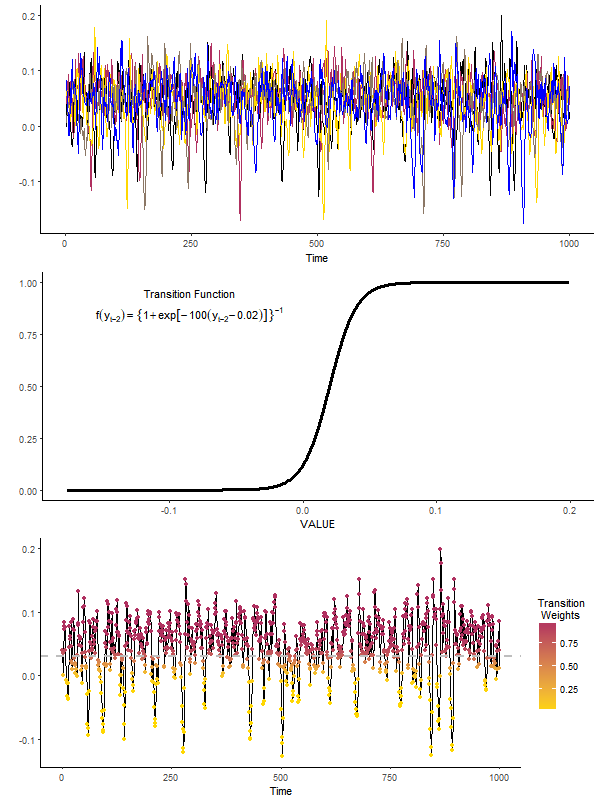
\includegraphics[scale=.7]{sim1plots}
	\label{fig:sim1plots}
\end{figure}

 This model is identical to the one presented in \cite{Lopes2006} where RJMCMC is used to select model order and a discrete $Uniform$ is adopted for $d$. If $p=4$ is known \textit{a priori}, the true parameter vector $\bm{\theta}=[\alpha_0, \alpha_1, \cdots, \alpha_4, \beta_0,\cdots,\beta_4, \gamma,\delta,\sigma]'$ contains $5$ zero parameters. Until further notice, $d$ is assumed to be known while the focus is on the ability of Bayesian shrinkage to combat over-fitting.

Bayesian estimation of the underlying LSTAR(2) model compares  BLASSO, RS-BLASSO, VS-BLASSO, and BHS shrinkage priors to conventional Normal priors. For the variations of BLASSO, posterior medians are obtained \citep{Park2008}, whereas when BHS \citep{Carvalho2009} or Normal priors are used, point estimates are based on posterior means. After a burn-in period of 15,000 and a thinning of 10 to reduce autocorrelation and control computer memory usage, 1,000 initial samples are obtained for 3 chains from the joint posterior distribution. The ``potential scale reduction factor'' (PSRF($\theta$)) of \cite{Gelman1992} evaluates convergence across the three chains, and effective sample size (ESS($\theta$)) measures mixing efficiency for each parameter $\theta \in \bm{\theta}$.  If $\underset{\theta}{\max} \textrm{ PSRF}(\theta)<1.05$ and $\underset{\theta}{\min} \textrm{ ESS}(\theta)>150$, convergence criteria is met and our initial sample is sufficient; otherwise, posterior samples are added, a maximum of 20 times, with intermittent convergence checks. Posterior simulations are only considered valid whenever the convergence criteria is met. Upcoming sections will follow the same convergence and reporting standards. Prior hyper-parameters are intentionally chosen to be non-informative and starting values are either randomly chosen or over-dispersed. Specifically for $\gamma^*$, a non-informative log normal prior $LN(3,1)$ is selected for all  simulation experiments \citep{Gerlach2008}. 

Table  \ref{tab:blassobhssummary} provides summary statistics of the posterior estimates from replications that converged using all five prior specifications. Rather than reporting the standard deviation of the estimates, estimation error is summarized using $RMSE(\theta)=\sqrt{\sum(\hat{\theta}-\theta)^2/n}$. There is consistent overestimation and large uncertainty for $\gamma$ --- commonly reported in literature \citep{Livingston2017} --- with the worst results for BHS and Normal priors. Figure \ref{fig:blvsbh} plots posterior estimates of the autoregressive parameters $\hat{\bm{\alpha}}$ and $\hat{\bm{\beta}}$. Discerning between shrinkage estimation methods is difficult since signal detection is satisfactory for all 4 methods. The optimal choice may be determined solely on computational efficiency which is left for discussion in a future subsection. Clearly, substantial improvements can be seen over the default normal prior choice.

\begin{sidewaystable}[htbp]
	\small
  \centering
  \caption{Posterior Estimate Summary for Simulation 1}
    \begin{tabular}{cccccccccccc}
    \toprule
   & & \multicolumn{2}{c}{BLASSO} &\multicolumn{2}{c}{RS-BLASSO} &\multicolumn{2}{c}{VS-BLASSO}  & \multicolumn{2}{c}{BHS} & \multicolumn{2}{c}{Normal} \\
    \cline{3-4} \cline{5-6} \cline{7-8} \cline{9-10} \cline{11-12}\\
    Parameter & Actual & Mean  & RMSE &  Mean & RMSE & Mean & RMSE & Mean & RMSE & Mean & RMSE   \\
    \midrule
   $\alpha_0$ & 0    & 0.0011 & 0.0024 & 0.0011 & 0.0025 & 0    & 0    & 0.0007 & 0.002 & 0.0049 & 0.0054 \\
    $\alpha_1$ & 1.8  & 1.7666 & 0.0715 & 1.7696 & 0.068 & 1.7765 & 0.0624 & 1.768 & 0.0746 & 1.5165 & 0.2898 \\
    $\alpha_2$ & -1.06 & -1.0046 & 0.1003 & -1.0108 & 0.0924 & -1.0367 & 0.081 & -1.0104 & 0.1159 & -0.5786 & 0.4888 \\
    $\alpha_3$ & 0    & -0.0042 & 0.0103 & -0.0026 & 0.0066 & 0.0007 & 0.0237 & -0.0125 & 0.0434 & -0.1745 & 0.1878 \\
    $\alpha_4$ & 0    & -0.004 & 0.0142 & -0.0027 & 0.0105 & -0.0022 & 0.0155 & -0.0028 & 0.031 & -0.0125 & 0.0618 \\
    $\beta_0$ & 0.02 & 0.0199 & 0.0039 & 0.0201 & 0.0067 & 0.0205 & 0.0032 & 0.0202 & 0.0035 & 0.021 & 0.0043 \\
    $\beta_1$ & 0.9  & 0.8714 & 0.0772 & 0.8697 & 0.1069 & 0.8987 & 0.0475 & 0.8899 & 0.0528 & 0.8635 & 0.0661 \\
    $\beta_2$ & -0.265 & -0.2246 & 0.0732 & -0.2253 & 0.0748 & -0.2684 & 0.0406 & -0.2496 & 0.053 & -0.2366 & 0.0584 \\
    $\beta_3$ & 0    & -0.0075 & 0.0139 & -0.0057 & 0.0114 & 0    & 0    & -0.0081 & 0.0296 & -0.0083 & 0.0504 \\
    $\beta_4$ & 0    & -0.0005 & 0.0151 & -0.0009 & 0.012 & -0.0003 & 0.0132 & 0.0019 & 0.0253 & 0.0033 & 0.0404 \\
    $\sigma$ & 0.02 & 0.0202 & 0.0004 & 0.0202 & 0.0004 & 0.0201 & 0.0004 & 0.0201 & 0.0004 & 0.021 & 0.0011 \\
    $\gamma$ & 100  & 131.0624 & 80.8034 & 131.5355 & 82.1307 & 131.0224 & 77.9754 & 174.15 & 148.8093 & 225.5381 & 204.5109 \\
    $\delta$ & 0.02 & 0.0218 & 0.0049 & 0.0218 & 0.0056 & 0.0204 & 0.0035 & 0.0208 & 0.0038 & 0.0261 & 0.0083 \\
    \bottomrule
    \end{tabular}%
  \label{tab:blassobhssummary}%
\end{sidewaystable}%

\begin{figure}[!h]
	\centering
	      \caption{Plot of $\hat{\bm{\alpha}}$ and $\hat{\bm{\beta}}$ for Simulation 1 }
      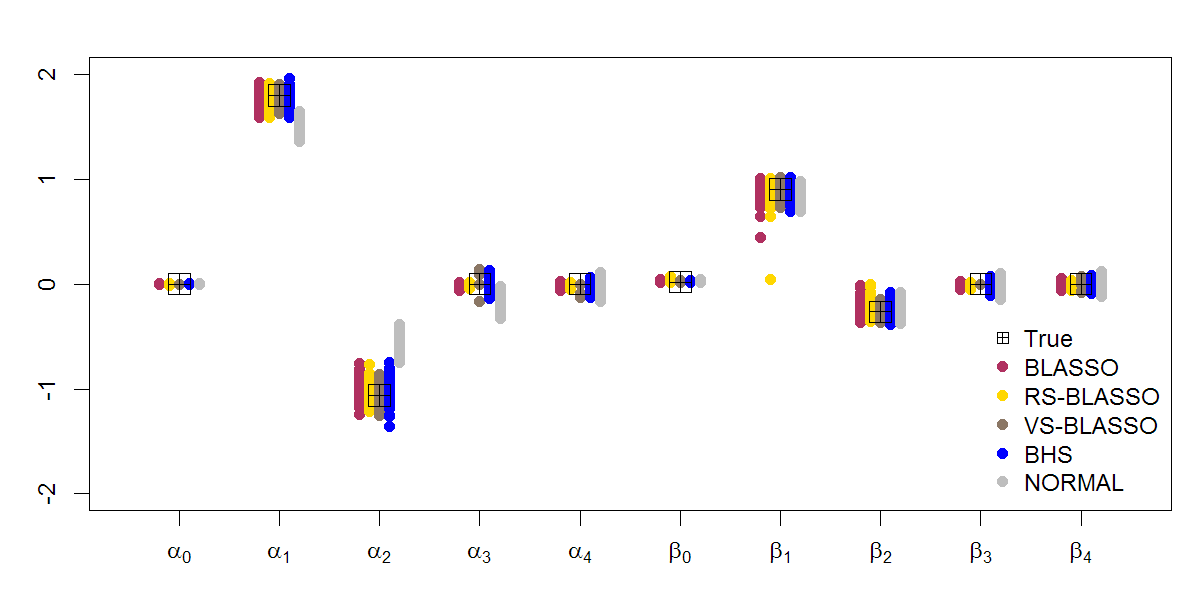
\includegraphics[scale=0.35]{blassovsbhs}
      \label{fig:blvsbh}
\end{figure}

Comparing our results to \cite{Lopes2006} is difficult for a number of reasons. For 50 replications, they obtain one MCMC chain of 2,500 posterior samples after a burn-in of 5,000; prior hyper-parameters are not specified and initial values are fixed. In this well-behaved case, posterior model probabilities pointed to the correct model 49 out of 50 times. For each replication, estimates are only based on the posterior samples where RJMCMC visited the correct LSTAR(2) model; no information is given on how many of the 2,500 posterior samples come from the correct parameter space. In \cite{Lopes2006}, overall summaries are based on the standard deviation (SD) of posterior estimates, whereas RMSE is evaluated here. The SD summarizes how much the posterior estimates differed from each other, while RMSE shows how much the posterior estimates differed from the truth. The main purpose for repeating this study is not to compare RJMCMC to Bayesian shrinkage but to establish the efficacy of these alternative methods for estimating a relatively simple LSTAR model. 

\subsection{Simulation 2: LSTAR with Gaps and Incremental Changes to Error Variance}
The next experiment is based on 100 replications of the LSTAR(3) model described in Equation \ref{eq:sim2}.
 \begin{equation}
	\begin{split}
		\label{eq:sim2}
		y_t&=(-0.6y_{t-3})[1-G(y_{t-1})] +(0.02+0.75y_{t-3})[G(y_{t-1})]+\epsilon_t\\
		& \textrm{where: } G(y_{t-1})=\bigg\{1+\exp\big[-120(y_{t-1}-0.02)\big]\bigg\}^{-1} \\
		&\textrm{ and }\epsilon_t \sim \textrm{i.i.d. }  N (0,0.02^2)\\
	\end{split}
\end{equation}

\begin{figure}
	\centering
	\caption{Ten Random Replications (top), Transition Function (middle), and Illustration of Regime-switching Behavior  for Simulation 2}
	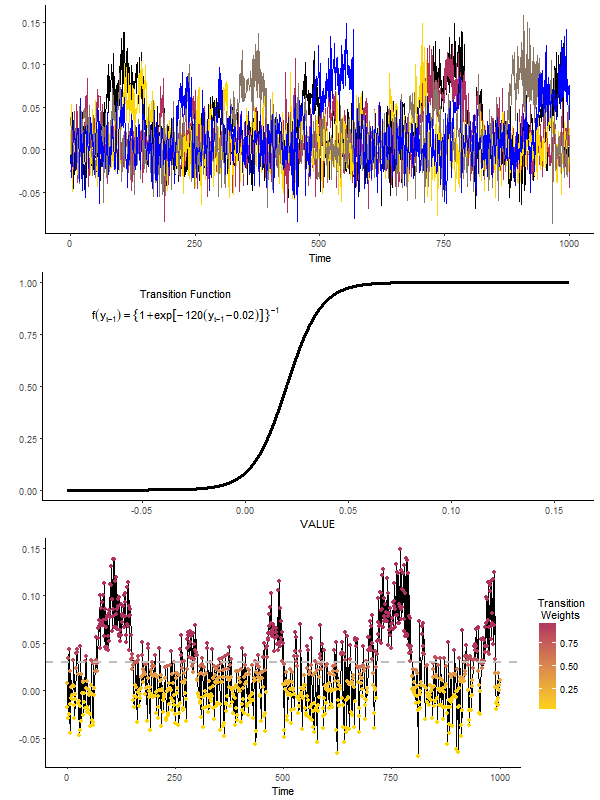
\includegraphics[scale=.7]{sim2plots}
	\label{fig:sim2plots}
\end{figure}

 Under the assumption that $p=4$, coefficients  $\bm{\theta}$ for autoregressive lags less than and larger than 3 are truly zero. This is a situation where even if RJMCMC visits the correct parameter space, normal priors will result in over-fitting. Motivation is geared towards nonlinear models where seasonal dynamics, of any period length, exhibit nonlinearities through dependence on some threshold variable.

Table \ref{tab:blassobhssummary3} summarizes and Figure \ref{fig:blvsbh3} illustrates the estimation accuracy of each method. Again, the normal priors result in unsatisfactory estimation accuracy. The simplest shrinkage methods, BLASSO and RS-BLASSO, consistently identify the true signal slightly better than the other shrinkage methods. 

\begin{sidewaystable}[htbp]
	\small
  \centering
  \caption{Posterior Estimate Summary for Simulation 2}
  \begin{tabular}{cccccccccccc}
    \toprule
   & & \multicolumn{2}{c}{BLASSO} &\multicolumn{2}{c}{RS-BLASSO} &\multicolumn{2}{c}{VS-BLASSO}  & \multicolumn{2}{c}{BHS} & \multicolumn{2}{c}{Normal} \\
    \cline{3-4} \cline{5-6} \cline{7-8} \cline{9-10} \cline{11-12}\\
    Parameter & Actual & Mean  & RMSE &  Mean & RMSE & Mean & RMSE & Mean & RMSE & Mean & RMSE   \\
    \midrule
    $\alpha_0$ & 0    & 0.0003 & 0.0011 & 0.0002 & 0.0011 & 0    & 0    & 0.0002 & 0.001 & 0.0041 & 0.0042 \\
    $\alpha_1$ & 0    & 0.0016 & 0.0097 & 0.0008 & 0.0051 & -0.0003 & 0.0157 & 0.0018 & 0.0273 & 0.2484 & 0.2556 \\
    $\alpha_2$ & 0    & 0.0004 & 0.007 & 0.0003 & 0.0041 & 0.0011 & 0.0094 & 0.0008 & 0.0154 & -0.0014 & 0.0517 \\
    $\alpha_3$ & -0.6 & -0.583 & 0.0547 & -0.5838 & 0.0544 & -0.5849 & 0.0548 & -0.5896 & 0.0537 & -0.2916 & 0.313 \\
    $\alpha_4$ & 0    & -0.0012 & 0.0073 & -0.0007 & 0.0044 & 0.0011 & 0.0075 & -0.0016 & 0.0149 & 0.0114 & 0.0529 \\
    $\beta_0$ & 0.02 & 0.0201 & 0.0019 & 0.0201 & 0.0018 & 0.0206 & 0.0021 & 0.0203 & 0.0021 & 0.0011 & 0.0195 \\
    $\beta_1$ & 0    & 0.0004 & 0.0051 & 0.0004 & 0.0044 & -0.0032 & 0.022 & -0.0022 & 0.0214 & 0.4269 & 0.4386 \\
    $\beta_2$ & 0    & 0.0005 & 0.0097 & 0.0006 & 0.0086 & 0.0016 & 0.0167 & 0.0002 & 0.0204 & 0.0008 & 0.0673 \\
    $\beta_3$ & 0.75 & 0.7307 & 0.046 & 0.73 & 0.0463 & 0.7306 & 0.0467 & 0.734 & 0.0439 & 0.5085 & 0.2764 \\
    $\beta_4$ & 0    & -0.0001 & 0.0067 & 0.0001 & 0.006 & -0.0004 & 0.0103 & -0.0012 & 0.0159 & -0.0113 & 0.0648 \\
    $\sigma$ & 0.02 & 0.0201 & 0.0004 & 0.0201 & 0.0004 & 0.0201 & 0.0004 & 0.02 & 0.0004 & 0.0232 & 0.0033 \\
    $\gamma$ & 120  & 130.5062 & 19.0649 & 130.3244 & 18.9201 & 128.4834 & 17.3982 & 130.9414 & 19.6161 & 686.7313 & 908.9353 \\
    $\delta$ & 0.02 & 0.0202 & 0.0013 & 0.0202 & 0.0013 & 0.0202 & 0.0013 & 0.0202 & 0.0013 & 0.025 & 0.007 \\
    \bottomrule
    \end{tabular}%
  \label{tab:blassobhssummary3}%
\end{sidewaystable}%

\begin{figure}[h]
	\centering
	      \caption{Plot of $\hat{\bm{\alpha}}$ and $\hat{\bm{\beta}}$ for Simulation 2}
      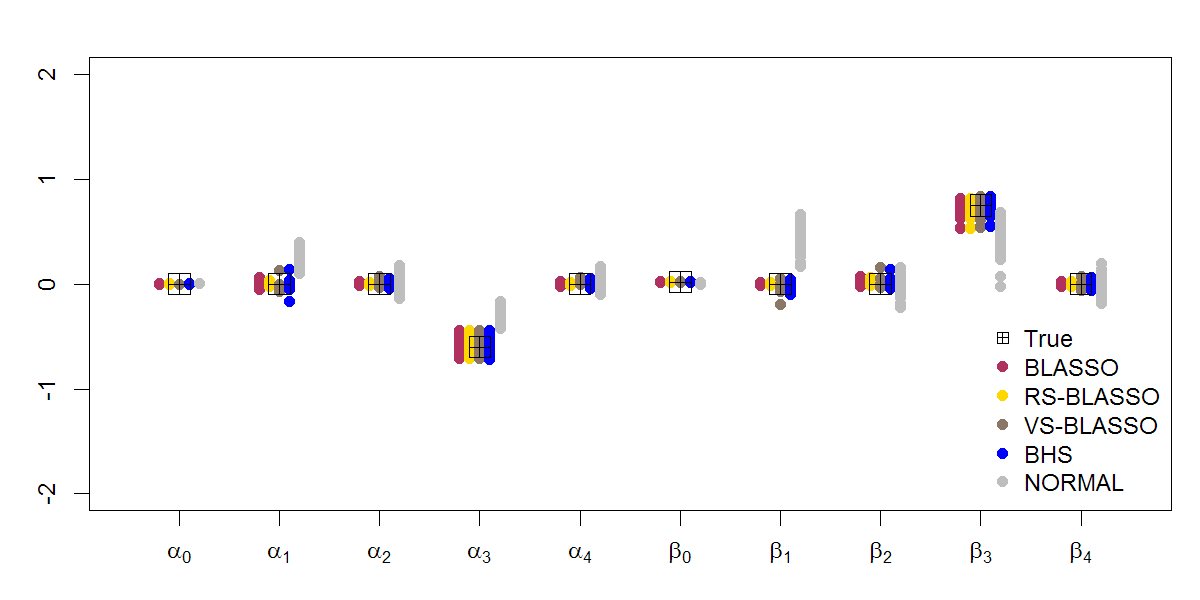
\includegraphics[scale=0.35]{blassovsbhs3}
      \label{fig:blvsbh3}
\end{figure}

Additionally, Simulation 2 is modified to allow $\sigma_k=0.02k$ $\forall k \in \{1,2,\cdots, 5\}$. For 50 replicates under each proposed $\sigma$, BLASSO and BHS methods are applied.  RMSE($\theta$) is naturally expected to increase with $\sigma$. The desire is to explore the sensitivity of RMSE($\theta$) as the noise is amplified. Under a fixed transition slope $\gamma=120$,  a contradictory trend was initially observed for known nonzero parameters $\alpha_3$ and $\beta_3$.  In Table \ref{tab:changingsigma}, RMSE($\alpha_3$) and RMSE($\beta_3$) gradually decline when $\gamma$ is fixed implying improved estimation. Increasing $\sigma$ naturally increases the sample standard deviation $s_{y}$. Under the reparameterization $\gamma=\gamma^*/s_y$, the unscaled transition slope $\gamma^*$ naturally must increase with $s_y$ to obtain the predetermined $\gamma=120$. 

Clearly, changing $\sigma$ has an impact on $\gamma^*$ through $s_y$. Although the actual transition function is not changing with $\sigma$ since it is fully determined by $\gamma$ and $\delta$, the speed of transition is increasing due to the natural modifications in the scope of the simulated data. The change is more visual in this regard. Therefore, for target $\gamma^*\approx 4$, data is simulated with $\gamma_k \approx 4/s_y$. Since $\sigma$ will naturally not equal $s_y$, the initial replications for each $\sigma_k$ under fixed $\gamma=120$ were used to obtain a mean estimate of $s_y$. Then, an appropriate $\gamma_k$ is determined for each $\sigma_k$, and 50 new replications are obtained. Table \ref{tab:changingsigma} shows the RMSE($\theta$) of each parameter for the specified options of $\sigma$ under fixed $\gamma_k=120$ and modified $\gamma_k$ to target $\gamma^*=4$. From these changes to the simulated data, RMSE($\alpha_3$) and RMSE($\beta_3$) increase with $\sigma_k$. Interestingly, the pattern for RMSE($\gamma$) is now reversed. These observations are  prevalent under both BLASSO and BHS priors; nevertheless, Bayesian shrinkage priors efficiently identify the nonlinear signal under gradual increases to the noise.




\begin{sidewaystable}[htbp]
\tiny
  \centering
  \caption{Sensitivity Analysis of RMSE($\bm{\theta}$) to $\sigma$ in Simulation 2}
    \begin{tabular}{cc|ccccc|ccccc}
    \toprule
    Method & Parameter & \multicolumn{5}{c}{Fixed Transition Slope} & \multicolumn{5}{c}{Modified Transition Slope} \\
    \midrule
    \multicolumn{2}{r|}{Choice of $\sigma$} & 0.02 & 0.04 & 0.06 & 0.08 & 0.1 & 0.02 & 0.04 & 0.06 & 0.08 & 0.1 \\
    \multicolumn{2}{r|}{Choice of $\gamma$} & \multicolumn{5}{c|}{$120$} & 109.60 & 71.47 & 49.50 & 37.46 & 30.02 \\
    \midrule
    BLASSO & $\alpha_0$ & 0.0009 & 0.0016 & 0.002 & 0.0025 & 0.0032 & 0.001 & 0.0016 & 0.0027 & 0.004 & 0.0049 \\
    & $\alpha_1$ &  0.0068 & 0.0104 & 0.0123 & 0.0145 & 0.013 & 0.0091 & 0.0141 & 0.0205 & 0.0248 & 0.0258 \\
    & $\alpha_2$ & 0.0125 & 0.0116 & 0.0102 & 0.0108 & 0.0102 & 0.0121 & 0.0136 & 0.0117 & 0.0127 & 0.0136 \\
    & $\alpha_3$ & 0.0479 & 0.0443 & 0.0383 & 0.0324 & 0.0328 & 0.0501 & 0.0522 & 0.055 & 0.0552 & 0.0543 \\
    & $\alpha_4$ & 0.0119 & 0.0128 & 0.008 & 0.0089 & 0.0106 & 0.012 & 0.0109 & 0.0097 & 0.0097 & 0.0099 \\
    & $\beta_0$ & 0.0019 & 0.0025 & 0.0038 & 0.0048 & 0.0059 & 0.0019 & 0.0027 & 0.0042 & 0.0057 & 0.0069 \\
    & $\beta_1$ & 0.006 & 0.0099 & 0.0152 & 0.0171 & 0.0177 & 0.0069 & 0.0066 & 0.0195 & 0.0227 & 0.0218 \\
    & $\beta_2$ & 0.0091 & 0.0147 & 0.0165 & 0.0154 & 0.0151 & 0.0127 & 0.0141 & 0.0154 & 0.0181 & 0.02 \\
    & $\beta_3$ & 0.0494 & 0.0429 & 0.0427 & 0.0438 & 0.0403 & 0.0579 & 0.061 & 0.0651 & 0.0683 & 0.0707 \\
    & $\beta_4$ & 0.008 & 0.0163 & 0.0136 & 0.0148 & 0.0204 & 0.0093 & 0.0202 & 0.0209 & 0.0195 & 0.0193 \\
    & $\sigma$ & 0.0005 & 0.0009 & 0.0014 & 0.0018 & 0.0023 & 0.0005 & 0.0009 & 0.0014 & 0.0018 & 0.0023 \\
    & $\gamma$ & 18.1887 & 23.4943 & 32.6301 & 32.8937 & 45.224 & 17.961 & 12.7347 & 9.5208 & 8.1114 & 7.1989 \\
    & $\delta$ & 0.0013 & 0.0019 & 0.0021 & 0.0025 & 0.0025 & 0.0013 & 0.0022 & 0.0038 & 0.0052 & 0.0065 \\
    \midrule
    HS & $\alpha_0$ & 0.0011 & 0.002 & 0.0028 & 0.0036 & 0.0049 & 0.0011 & 0.002 & 0.0033 & 0.0049 & 0.0065 \\
    & $\alpha_1$ & 0.0054 & 0.0127 & 0.0186 & 0.0236 & 0.0251 & 0.0063 & 0.0144 & 0.0233 & 0.03 & 0.0345 \\
    & $\alpha_2$ & 0.0075 & 0.013 & 0.0157 & 0.018 & 0.0181 & 0.0074 & 0.0141 & 0.0162 & 0.0192 & 0.0223 \\
    & $\alpha_3$ & 0.0485 & 0.0451 & 0.0386 & 0.0329 & 0.0334 & 0.0508 & 0.0545 & 0.0575 & 0.0576 & 0.0568 \\
   & $\alpha_4$ & 0.0079 & 0.0139 & 0.0138 & 0.0155 & 0.0174 & 0.008 & 0.0134 & 0.0159 & 0.0181 & 0.02 \\
    & $\beta_0$ & 0.0018 & 0.0024 & 0.0037 & 0.0046 & 0.0058 & 0.0018 & 0.0026 & 0.0039 & 0.0053 & 0.0067 \\
    & $\beta_1$ & 0.004 & 0.0111 & 0.0151 & 0.0204 & 0.0242 & 0.0039 & 0.0081 & 0.0162 & 0.022 & 0.0258 \\
    & $\beta_2$ & 0.0068 & 0.0152 & 0.0196 & 0.0214 & 0.0237 & 0.0071 & 0.014 & 0.0189 & 0.0226 & 0.0261 \\
   & $\beta_3$ & 0.0524 & 0.044 & 0.0442 & 0.0451 & 0.042 & 0.0608 & 0.0642 & 0.0688 & 0.072 & 0.0739 \\
    & $\beta_4$ & 0.0062 & 0.0164 & 0.0181 & 0.0215 & 0.0258 & 0.0063 & 0.0183 & 0.0227 & 0.024 & 0.0259 \\
    & $\sigma$ & 0.0005 & 0.0009 & 0.0014 & 0.0018 & 0.0023 & 0.0005 & 0.0009 & 0.0014 & 0.0018 & 0.0023 \\
   & $\gamma$ & 19.0596 & 24.0976 & 33.568 & 33.4267 & 45.3324 & 19.0212 & 13.5966 & 10.205 & 8.596 & 7.5575 \\
   & $\delta$ & 0.0013 & 0.0019 & 0.0021 & 0.0025 & 0.0025 & 0.0014 & 0.0022 & 0.0038 & 0.0052 & 0.0065 \\
    \bottomrule
    \end{tabular}%
  \label{tab:changingsigma}%
\end{sidewaystable}%


\subsection{Simulation 3: LSTAR with Regime-Specific Sparsity}

The effectiveness of the proposed methods is evaluated via simulating 100 replicates of the LSTAR(3) model in Equation \ref{eq:sim3}, exhibiting regime-specific complexity: the autoregressive dynamics are far simpler in the low regime relative to the high regime.
 \begin{equation}
	\begin{split}
		\label{eq:sim3}
		y_t&=(-0.7y_{t-3})[1-G(y_{t-1})] \\
		& +(0.06+0.4y_{t-1}-0.35y_{t-2}+0.2y_{t-3})[G(y_{t-1})]+\epsilon_t\\
		& \textrm{where: } G(y_{t-1})=\bigg\{1+\exp\big[-120(y_{t-1}-0.03)\big]\bigg\}^{-1} \\
		&\textrm{ and }\epsilon_t \sim \textrm{i.i.d. }  N (0,0.02^2)\\
	\end{split}
\end{equation}
\begin{figure}
	\centering
	\caption{Ten Random Replications (top), Transition Function (middle), and Illustration of Regime-switching Behavior  for Simulation 3}
	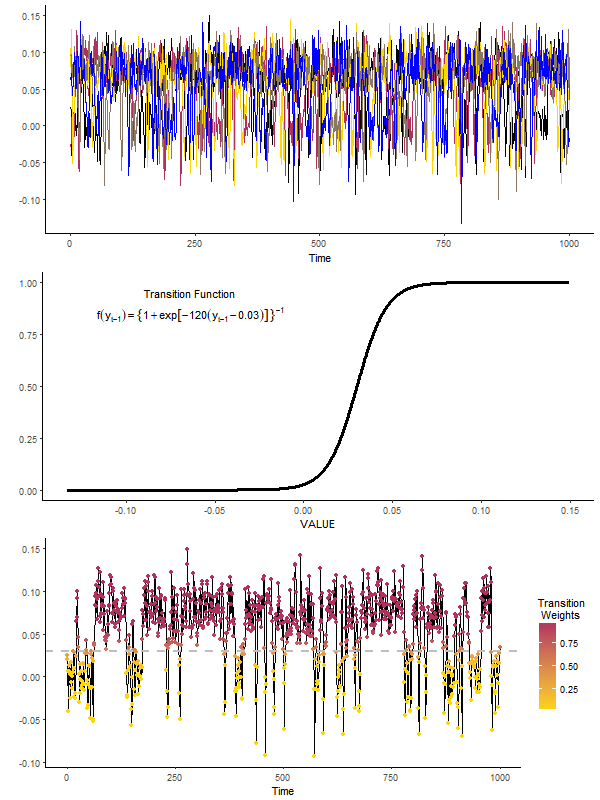
\includegraphics[scale=.7]{sim3plots}
	\label{fig:sim3plots}
\end{figure}
From Table \ref{tab:blassobhssummary4} and Figure \ref{fig:blvsbh4}, one observes that estimation accuracy is satisfactory for all three shrinkage methods, whereas $Normal$ priors continue to lead to poor estimates. The motivation for regime-specific shrinkage parameters $\lambda_1$ and $\lambda_2$ is illustrated in Figure \ref{fig:lambdabox}, which presents histograms of posterior median estimates for the tuning parameters of BLASSO vs RS-BLASSO. The visual disparity between $\lambda_1$ and $\lambda_2$ is a result of the regime-specific sparsity patterns: $\lambda_1>\lambda_2$ necessitates from the lower regime requiring relatively more shrinkage to identify the underlying signal.

\begin{sidewaystable}[htbp]
	\scriptsize
  \centering
  \caption{Posterior Estimate Summary for Simulation 3}
  \begin{tabular}{cccccccccccc}
    \toprule
   & & \multicolumn{2}{c}{BLASSO} &\multicolumn{2}{c}{RS-BLASSO} &\multicolumn{2}{c}{VS-BLASSO}  & \multicolumn{2}{c}{BHS} & \multicolumn{2}{c}{Normal} \\
    \cline{3-4} \cline{5-6} \cline{7-8} \cline{9-10} \cline{11-12}\\
    Parameter & Actual & Mean  & RMSE &  Mean & RMSE & Mean & RMSE & Mean & RMSE & Mean & RMSE   \\
    \midrule
   $\alpha_0$ & 0    & -0.0003 & 0.0019 & 0    & 0.0017 & 0    & 0.0003 & 0    & 0.002 & 0.0125 & 0.0126 \\
    $\alpha_1$ & 0    & 0.0011 & 0.0092 & 0.0003 & 0.0026 & -0.0004 & 0.0151 & 0.003 & 0.0431 & 0.6015 & 0.6135 \\
    $\alpha_2$ & 0    & -0.0031 & 0.0123 & -0.0006 & 0.0035 & -0.0035 & 0.0244 & -0.0058 & 0.0375 & -0.093 & 0.1118 \\
    $\alpha_3$ & -0.7 & -0.6785 & 0.0448 & -0.6816 & 0.0439 & -0.6754 & 0.052 & -0.6803 & 0.0553 & -0.4609 & 0.2483 \\
    $\alpha_4$ & 0    & -0.0016 & 0.0131 & -0.0005 & 0.0044 & -0.0008 & 0.0118 & -0.0026 & 0.0311 & -0.056 & 0.1002 \\
    $\beta_0$ & 0.06 & 0.0612 & 0.0046 & 0.0613 & 0.0042 & 0.061 & 0.0042 & 0.0609 & 0.0042 & 0.0301 & 0.0305 \\
    $\beta_1$ & 0.4  & 0.3692 & 0.0674 & 0.37 & 0.0613 & 0.3802 & 0.0545 & 0.3809 & 0.056 & 0.7792 & 0.3863 \\
    $\beta_2$ & -0.35 & -0.3054 & 0.0695 & -0.3005 & 0.0717 & -0.3292 & 0.0508 & -0.3242 & 0.0536 & -0.3312 & 0.0501 \\
    $\beta_3$ & 0.2  & 0.1597 & 0.0596 & 0.1538 & 0.0643 & 0.1844 & 0.0375 & 0.1766 & 0.0454 & 0.1371 & 0.0771 \\
    $\beta_4$ & 0    & 0.0104 & 0.0202 & 0.0101 & 0.0198 & 0.0015 & 0.0128 & 0.0063 & 0.0225 & -0.0087 & 0.039 \\
    $\sigma$ & 0.02 & 0.0202 & 0.0005 & 0.0202 & 0.0004 & 0.0201 & 0.0004 & 0.0201 & 0.0004 & 0.0239 & 0.0039 \\
    $\gamma$ & 120  & 120.5942 & 9.7438 & 121.8142 & 10.8705 & 121.3552 & 10.2547 & 123.1839 & 11.4902 & 617.4922 & 740.3125 \\
    $\delta$ & 0.03 & 0.0302 & 0.0011 & 0.0303 & 0.0011 & 0.0303 & 0.001 & 0.0302 & 0.0011 & 0.0378 & 0.0089 \\
    \bottomrule
    \end{tabular}%
  \label{tab:blassobhssummary4}%
\end{sidewaystable}%

\begin{figure}[!h]
	\centering
	      \caption{Plot of $\hat{\bm{\alpha}}$ and $\hat{\bm{\beta}}$ for Simulation 3}
      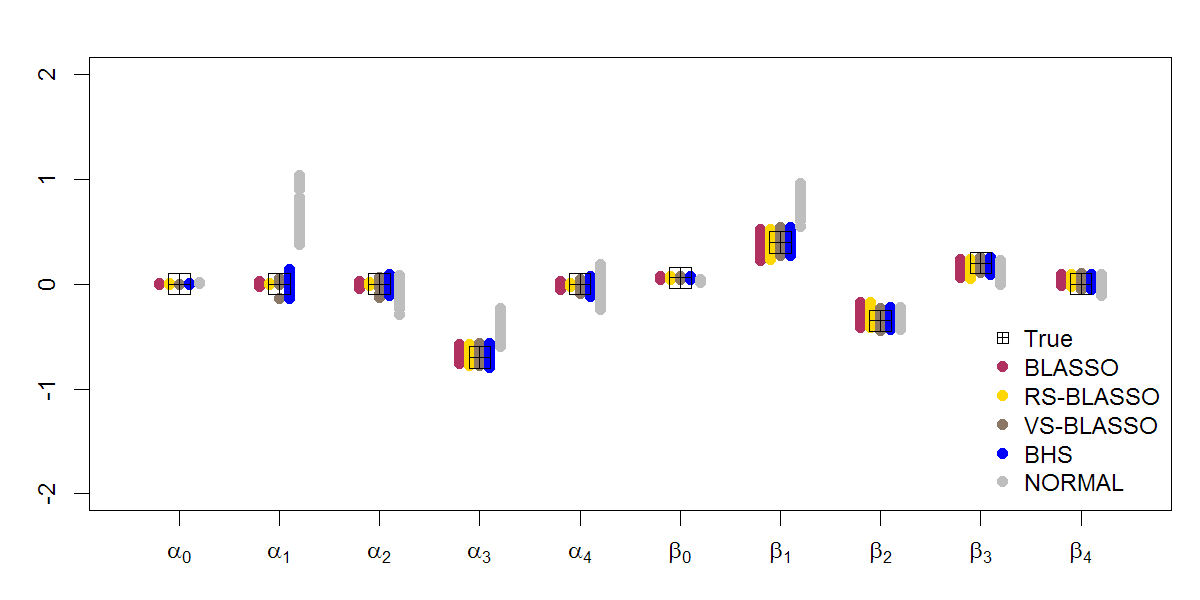
\includegraphics[scale=0.35]{blassovsbhs4}
      \label{fig:blvsbh4}
\end{figure}

\begin{figure}[!h]
	\centering
	      \caption{Posterior Shrinkage Comparison for BLASSO vs RS-BLASSO}
      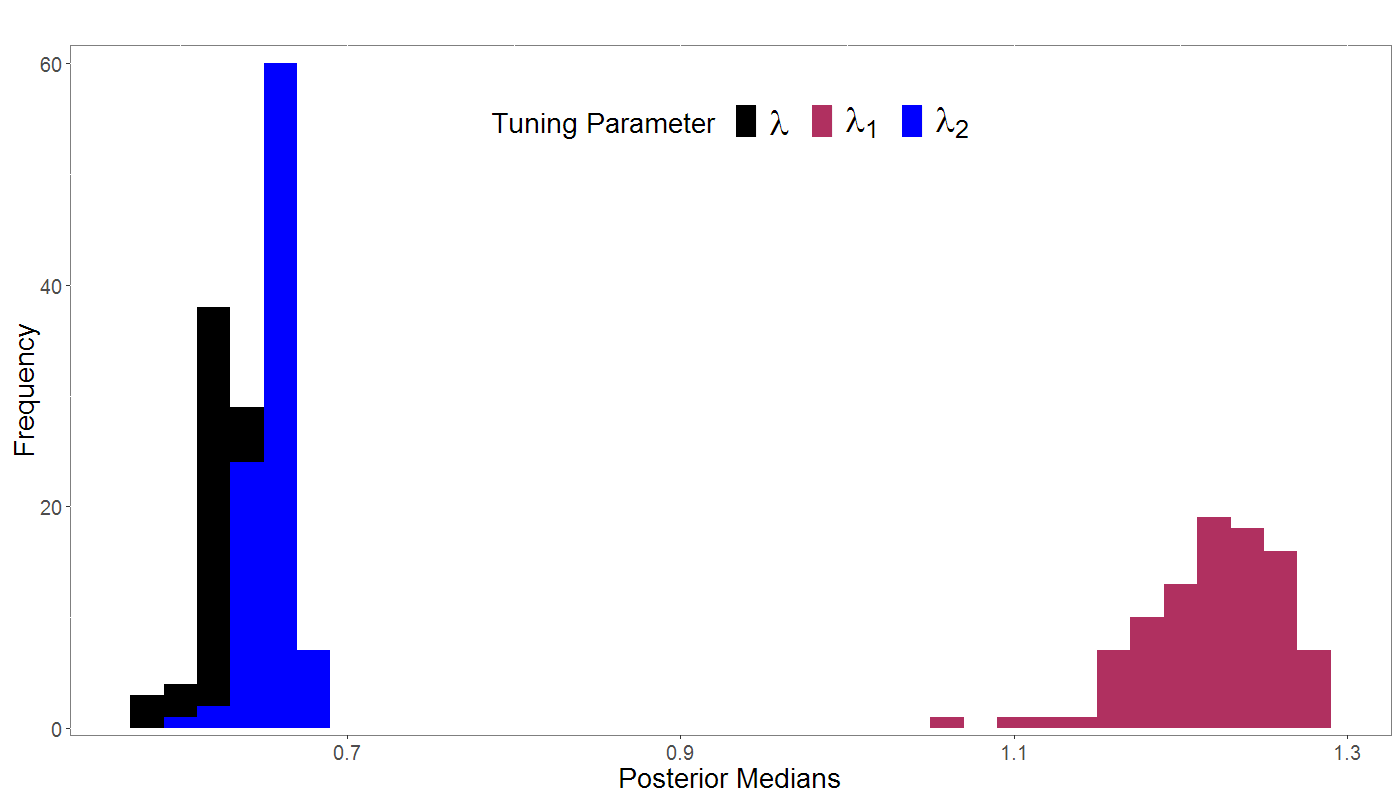
\includegraphics[scale=0.30]{rslambda}
      \label{fig:lambdabox}
\end{figure}

\vskip 3mm

\subsection{Convergence Analysis}

Simulations 1-3 were conducted on an Intel(R) Xeon (R) CPU E5-2697 v3 @ 2.60 GHz server with 132GB of RAM and 56 cores. Both the replications and the MCMC chains were parallel-processed within limitations of the server. The resources were often shared amongst colleagues, hence computational times can be misleading as a measure of efficiency. Since the parameter space is fixed for each MCMC routine, efficiency can be measured by the number of posterior samples required to attain the convergence criteria. Table \ref{tab:convtable} reports the percent of the 100 replications that converged along with the mean, median, and extreme percentiles of the samples required for the replications that converged.

When the model order $p$ is overestimated, the four shrinkage methods resist over-fitting to identify the true nonlinear process; therefore, choosing a method in practice ultimately depends on computational feasibility. All methods were equally efficient for Simulation 2 and unaffected by changes in noise. The methods were organized in order of regularization flexibility. For Simulations 1 and 3, the percent of converged replicates increased with the aforementioned flexibility. Specifically for Simulation 3, the additional tuning parameter in RS-BLASSO increased this percentage by 19\%, identifying the true advantage for regime-specific shrinkage. The BHS hierarchy is commended for being consistently efficient.

\begin{table}[!h]
\scriptsize
  \centering
  \caption{Convergence Statistics for Estimation Methods From Simulations 1-3}
    \begin{tabular}{cc|c|cccc}
    \toprule
    & & Percent of Replications & \multicolumn{4}{c}{Summary Statistics of Samples Required}\\
    Simulation & Method & Converged  & 5th Percentile   & Mean & Median & 95th Percentile \\
    \midrule
    1    & BLASSO & 91\%   & 1000 & 11615 & 2000 & 67000 \\
    1    & RS-BLASSO & 96\%    & 1000 & 10188 & 2000 & 110125 \\
    1    & VS-BLASSO & 99\%    & 1000 & 3202 & 2000 & 11000 \\
    1    & BHS  & 100\%   & 1000 & 1600 & 1000 & 4000 \\
    1    & Normal & 100\%   & 1000 & 1360 & 1000 & 4000 \\
    \midrule
    2    & BLASSO & 100\%   & 1000 & 1000 & 1000 & 1000 \\
    2    & RS-BLASSO & 100\%   & 1000 & 1000 & 1000 & 1000 \\
    2    & VS-BLASSO & 100\%   & 1000 & 2120 & 1000 & 4000 \\
    2    & BHS  & 100\%   & 1000 & 1010 & 1000 & 1000 \\
    2    & Normal & 100\%   & 1000 & 1150 & 1000 & 3050 \\
    \midrule
    3    & BLASSO & 75\%    & 1000 & 15800 & 2000 & 131500 \\
    3    & RS-BLASSO & 94\%    & 1000 & 1723 & 1000 & 4000 \\
    3    & VS-BLASSO & 100\%   & 1000 & 1380 & 1000 & 4000 \\
    3    & BHS  & 99\%    & 1000 & 1010 & 1000 & 1000 \\
    3    & Normal & 99\%    & 2000 & 8232 & 4000 & 46000 \\
    \bottomrule
    \end{tabular}%
  \label{tab:convtable}%
\end{table}%

\vskip 3mm

\subsection{Bayesian Selection of the Threshold Variable}

To incorporate the uncertainty for the delay $d$, Simulation 1 is revisited where the true threshold variable $y_{t-2}$ was assumed to be known. Maintaining the assumption $p = 4$, the vector $\bm{y}=[y_{t-1},y_{t-2},y_{t-3},y_{t-4}]'$ contains the threshold variables of interest. The re-paramaterized transition function $G(\bm{y})=\{1+\exp[-100(\bm{\phi}'\bm{y}-0.02)]\}^{-1}$ is equivalent to the transition function in Equation \ref{eq:sim1} when $\bm{\phi}=[\phi_1,\phi_2,\phi_3,\phi_4]'=[0,1,0,0]'$. Posterior sampling of $\bm{\phi}$ is combined with BLASSO and BHS under the previously stated convergence requirements. 

First, independent Bernoulli priors were used for $\phi_k$ along with BLASSO. Only 43\% of the replications converged compared to 91\% when $d=2$ was known. The average of the 43 posterior means for $\bm{\phi}$ was $[0.223,0.988,0.206,0.040]'$; the independent Bernoulli priors do not limit the threshold variable to one choice in  $\{y_{t-1},y_{t-2},y_{t-3},y_{t-4}\}$ since $\sum \phi_k \neq 1$ is not enforced. Estimation accuracy for non-$\bm{\phi}$ parameters was similar to the results presented in the previous Sections, but Bernoulli priors will not be discussed further due to computational deficiencies.

Next, let $\bm{\phi}\sim Dir([0.25,0.25,0.25,0.25]')$; the uninformative hyper-parameter demonstrates prior impartiality regarding $d$. BLASSO and BHS are combined with the $Dirichlet$ prior to re-estimate the 100 replications in Simulation 1, of which 98\% and 100\% converged, respectively. Table \ref{tab:rmsedirichlet} uses the RMSE of non-$\bm{\phi}$ parameters to show that MCMC sampling for $\bm{\phi}$ does not render the previous estimation methods useless. Table \ref{tab:estdirichlet} depicts summary statistics of the posterior means for $\bm{\phi}$ from the replications that converged. Figure \ref{fig:dirichlet1} overlays the posterior means summarized in Table \ref{tab:estdirichlet}. Both star plots heavily point toward the correct threshold variable indicating accurate estimation of $\bm{\phi}$. 
 
\begin{table}[!h]
	\footnotesize
  \centering
  \caption{Sensitivity of RMSE($\bm{\theta}$) to Uncertainty about $\bm{\phi}$ in Simulation 1}
    \begin{tabular}{cccccc}
    \toprule
    & \multicolumn{2}{c}{$\bm{\phi} \sim Dir$} & \multicolumn{2}{c}{$\bm{\phi}$ Known}\\
    \cline{2-3} \cline{4-5}
     Parameter & BLASSO & BHS & BLASSO & BHS  \\
    \midrule
    $\alpha_0$    & 0.0027 & 0.002 & 0.0024 & 0.002 \\
  $\alpha_1$  & 0.0763 & 0.0827 & 0.0715 & 0.0746 \\
    $\alpha_2$ & 0.1048 & 0.1269 & 0.1003 & 0.1159 \\
    $\alpha_3$    & 0.0103 & 0.038 & 0.0103 & 0.0434 \\
    $\alpha_4$    & 0.0153 & 0.0265 & 0.0142 & 0.031 \\
   $\beta_0$ & 0.0072 & 0.0034 & 0.0039 & 0.0035 \\
    $\beta_1$  & 0.1091 & 0.0541 & 0.0772 & 0.0528 \\
    $\beta_2$   & 0.0745 & 0.0549 & 0.0732 & 0.053 \\
   $\beta_3$     & 0.0147 & 0.0271 & 0.0139 & 0.0296 \\
    $\beta_4$    & 0.0156 & 0.0245 & 0.0151 & 0.0253 \\
   $\sigma$ & 0.0004 & 0.0004 & 0.0004 & 0.0004 \\
    $\gamma$  & 87.1606 & 91.2016 & 80.8034 & 148.8093 \\
    $\delta$ & 0.0058 & 0.004 & 0.0049 & 0.0038 \\
    \bottomrule
    \end{tabular}%
  \label{tab:rmsedirichlet}%
\end{table}%


\begin{table}[!h]
	\footnotesize
  \centering
  \caption{Posterior Estimate Summary for $\bm{\phi}$ in Simulation 1}
    \begin{tabular}{cccccccc}
    \toprule
    & & \multicolumn{3}{c}{BLASSO} & \multicolumn{3}{c}{ BHS} \\
    \cline{3-5} \cline{6-8}\\
   Parameter & Actual & 5th \%-ile   & Mean & 95th \%-ile   & 5th \%-ile   & Mean & 95th \%-ile \\
    \midrule
    $\phi_1$    & 0    & 0.0114 & 0.0557 & 0.1618 & 0.0110 & 0.0581 & 0.1920 \\
    $\phi_2$    & 1    & 0.6501 & 0.8686 & 0.9536 & 0.6008 & 0.8653 & 0.9527 \\
   $\phi_3$    & 0    & 0.0144 & 0.0465 & 0.1301 & 0.0143 & 0.0475 & 0.1254 \\
   $\phi_4$    & 0    & 0.0079 & 0.0292 & 0.0897 & 0.0082 & 0.0290 & 0.0810 \\
    \bottomrule
    \end{tabular}%
  \label{tab:estdirichlet}%
\end{table}%


\begin{figure}[!h]
\centering
\caption{Posterior Means of $\bm{\phi}$ for Simulation 1 Using BLASSO (left) and BHS (right)}
\begin{minipage}[h]{0.4\textwidth}
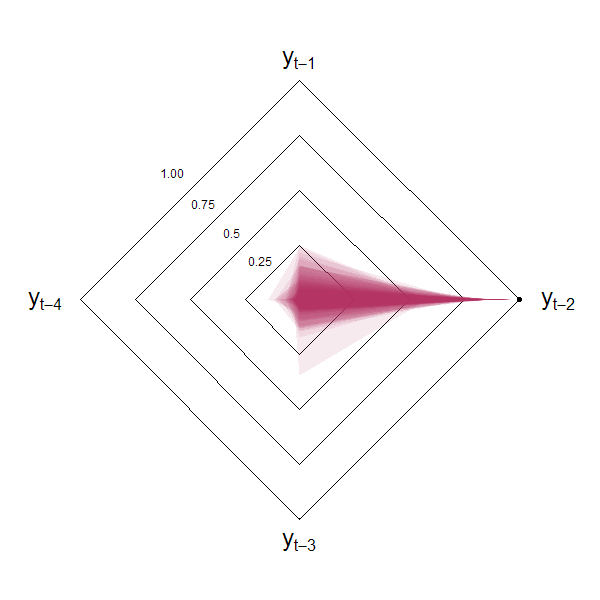
\includegraphics[scale=0.32]{blassodlp}
\end{minipage} \hspace{0.10\textwidth}
\begin{minipage}[h]{0.4\textwidth}
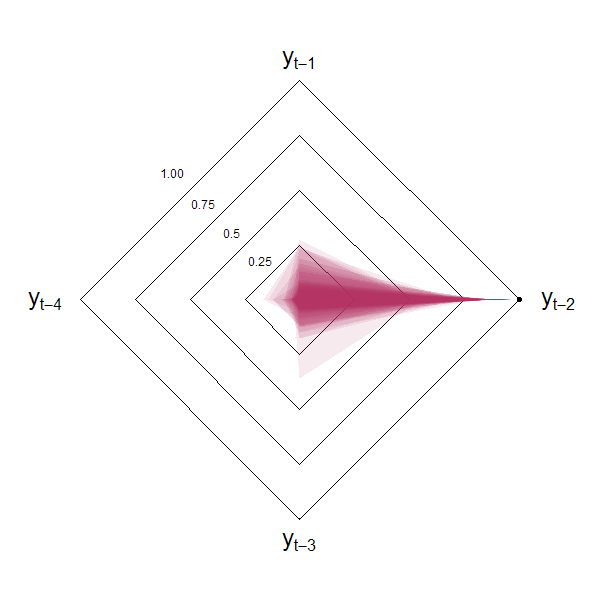
\includegraphics[scale=0.32]{hsdlp}
\end{minipage}
\label{fig:dirichlet1}
\end{figure}


Simulation 2 is repeated for three threshold variables denoted $z_{1,t},z_{2,t},$ and $z_{3,t}$ and identified in Equation \ref{eq:thvarchoice}. The first two threshold variables conform to the classic LSTAR structure; however, $z_{3,t}$ is an average of the first three lags of the endogenous time series $\bm{y_t}$. Conventional estimation of the delay $d$ would be unable to correctly identify $z_{3,t}$. Using BHS only, all 3 modifications are identifiable when a 4-dimensional $Dirichlet$ prior is used for $\bm{\phi}$.
 \begin{equation}
\label{eq:thvarchoice}
\begin{split}
	z_{1,t}&=y_{t-1}=\bm{\phi_1}'\bm{y}=[1,0,0,0]\bm{y}\\
	z_{2,t}&=y_{t-2}=\bm{\phi_2}'\bm{y}=[0,1,0,0]\bm{y}\\\
	z_{3,t}&=\frac{y_{t-1}+y_{t-2}+y_{t-3}}{3}=\bm{\phi_3}'\bm{y}=\bigg[\frac{1}{3},\frac{1}{3},\frac{1}{3},0\bigg]\bm{y}\\\
\end{split}
\end{equation}
Acknowledged uncertainty about the threshold variable manifests lower convergence rates than the original 100\% seen in Simulation 2. Based on 100 replications, convergence rates were 86\%, 75\%, and 87\% for  $z_{1,t}, z_{2,t},$ and $z_{3,t}$, respectively. For replications that converged, Figures 6-8 present posterior means of $\bm{\phi_k}$ for $k \in\{1,2,3\}$. Figure \ref{fig:th1} shows almost perfect posterior weighting towards the true $z_{1,t}=y_{t-1}$ while Figure \ref{fig:th2} provides evidence of occasional mis-identification of $z_{2,t}=y_{t-2}$. Figure \ref{fig:th3} for $z_{3,t}$ shows almost equal favor for $y_{t-1}$, $y_{t-2}$,  and $y_{t-3}$ while severely down-weighting $y_{t-4}$.

\begin{figure}[!h]
\center
\begin{minipage}[h]{0.4\textwidth}
\caption{Posterior Means of $\bm{\phi_1}$ When $z_{1,t}=y_{t-1}$}
\label{fig:th1}
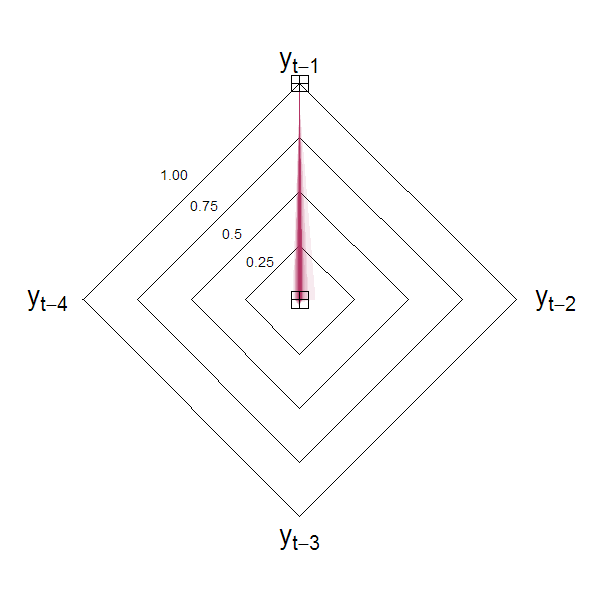
\includegraphics[scale=0.32]{hsthvar1}
\end{minipage} \hspace{0.1\textwidth}
\begin{minipage}[h]{0.4\textwidth}
\caption{Posterior Means of $\bm{\phi_2}$ When $z_{2,t}=y_{t-2}$}
\label{fig:th2}
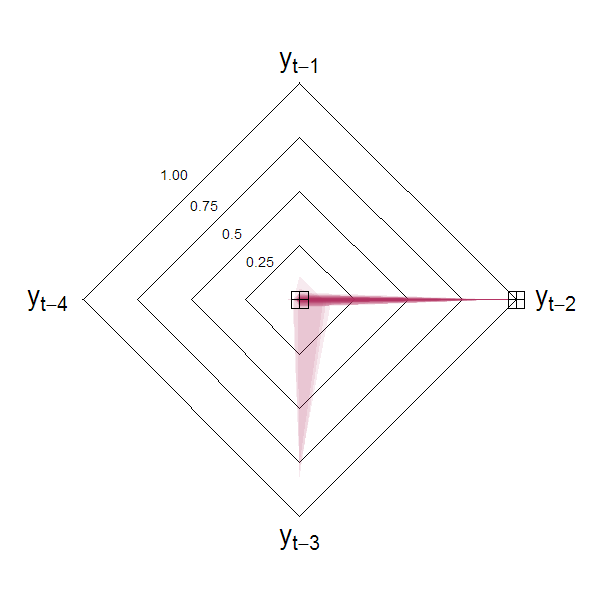
\includegraphics[scale=0.32]{hsthvar2}
\end{minipage}
\begin{minipage}[h]{0.8\textwidth}
\caption{Posterior Means of $\bm{\phi_3}$ When $z_{3,t}=\frac{y_{t-1}+y_{t-2}+y_{t-3}}{3}$}
\label{fig:th3}
\center
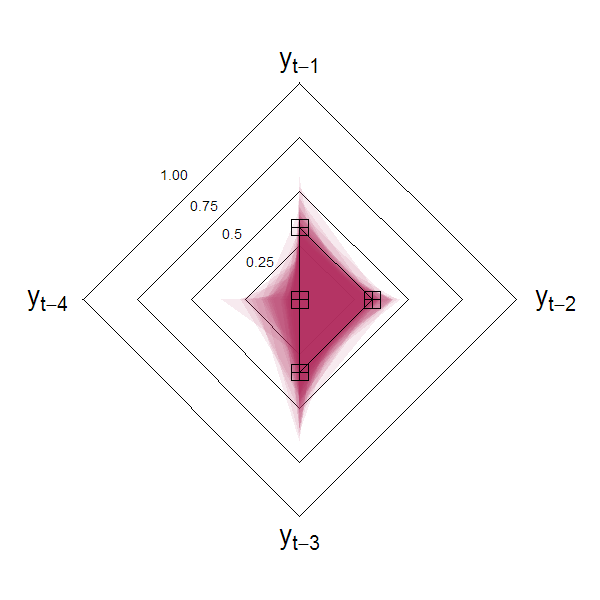
\includegraphics[scale=0.32]{hsthvar3}
\end{minipage}
\end{figure}


%%%%%%%%%%%%%%%%%%%%%%%%%%%%%%%%%%%%%%%%%%%%%%%%%%%%%%%%%%%%%%%


\section{Forecasting Annual Sunspot Numbers}

International sunspot numbers are gathered and updated by the World Data Center SILSO, Royal Observatory of Belgium, Brussels. Since \cite{Granger1957} , this data has served as an example in nonlinear time series literature. Letting $x_t$ represent the annual sunspot number at time $t$, the square root transformation $y_t= 2[\sqrt{1+x_t}-1]$ following \cite{Ghaddar1981} is applied. Data from 1700 to 1979 are used to estimate models while data from 1980 to 2006 are used to evaluate their forecasting accuracy. \cite{Terasvirta2010} compares three nonlinear time series models, namely STAR, TAR, and Artificial Neural Nets (AR-NN), to the baseline linear AR model. The LSTAR model in Equation \ref{eq:TModel} had optimal $h$-step ahead forecasting performance for horizons $h \in \{1,2,\cdots,5\}$. Sparsity is achieved through a stepwise frequentist procedure; henceforth, this model abbreviates to $F_T$. 
\begin{equation}
\begin{split}
 	y_t &=(1.46y_{t-1}-0.76y_{t-2}+0.17y_{t-7}+0.11y_{t-9})[1-G(y_{t-2},5.5,7.9)]\\
 	&+(2.7+0.92y_{t-1}-0.01y_{t-2}-0.47y_{t-3}+0.32y_{t-4}-0.26y_{t-5}\\
 	&+0.17y_{t-7}-0.24y_{t-8}+0.11y_{t-9}+0.17y_{t-10})G(y_{t-2},5.5,7.9)+\hat{\epsilon}_t\\
 	\textrm{where: } & \hat{\epsilon}_t \sim N(0, 1.898^2).\\
\end{split}
\label{eq:TModel}
\end{equation}
Simulation results indicate the difficulty of normal priors in combating over-fitting: even if RJMCMC directed to the correct model order $p=10$, current Bayesian approaches are incapable of estimating the model in Equation \ref{eq:TModel}. Assuming the delay $d=2$, a fully saturated LSTAR(10) model, denoted $F_S$, is estimated for a baseline comparison.

Hypothesis testing for the threshold variable produced ambiguous results as nonlinearity was rejected for multiple delay parameters. \cite{Terasvirta2010} chose $d=2$ based on p-value magnitude, but recommended LSTAR modeling for other values of $d$. Assuming $p=10$ and $d=2$, BHS priors estimate the LSTAR model, denoted $B_2$, in Equation \ref{eq:HSModel}. Posterior standard deviations are provided below the corresponding regime-specific AR coefficients. Parameter estimates for $\alpha_6$ and $\beta_6$ round to zero and are ignored from the model representation.
\begin{equation}
\begin{split}
 	y_t &=(-\underset{(1.14)}{0.56}+\underset{(0.20)}{1.56}y_{t-1}-\underset{(0.29)}{0.52}y_{t-2}+\underset{(0.15)}{0.01}y_{t-3}-\underset{(0.14)}{0.06}y_{t-4}\\
 	&-\underset{(0.12)}{0.03}y_{t-5} +\underset{(0.17)}{0.18}y_{t-7}+\underset{(0.13)}{0.05}y_{t-8}+\underset{(0.15)}{0.14}y_{t-9}-\underset{(0.10)}{0.04}y_{t-10})\\
 	&\times[1-G(y_{t-2},5.21,8.37)]+(\underset{(1.11)}{0.43}+\underset{(0.25)}{0.83}y_{t-1}+\underset{(0.28)}{0.14}y_{t-2}\\
 	&-\underset{(0.14)}{0.24}y_{t-3}+\underset{(0.11)}{0.06}y_{t-4}-\underset{(0.10)}{0.1}y_{t-5}
+\underset{(0.09)}{0.04}y_{t-7}-\underset{(0.14)}{0.13}y_{t-8}\\
&+\underset{(0.11)}{0.06}y_{t-9}+\underset{(0.10)}{0.14}y_{t-10})[G(y_{t-2},5.21,8.37)]+\hat{\epsilon}_t\\
 	\textrm{where: }  \hat{\epsilon}_t &\sim N(0, 1.94^2)\\
\end{split}
\label{eq:HSModel}
\end{equation}
Along with BHS priors, $\bm{\phi} \sim Dir ([\frac{1}{4},\frac{1}{4},\frac{1}{4},\frac{1}{4}]')$ for Bayesian estimation of the threshold variable $z_t=\bm{\phi}'\bm{y}$. Results from \cite{Terasvirta2010} indicate that $z_t \in \{y_{t-1},y_{t-2},y_{t-3},y_{t-4}\}$ is likely; therefore in the re-parameterization, let $\bm{y}=[y_{t-1},y_{t-2},y_{t-3},y_{t-4}]'$. The estimated model in Equation \ref{eq:HSModelDIR} provides conflicting results for $z_t$; this model is denoted $B_D$. Posterior mean of $\bm{\phi}$ places more weight on $y_{t-3}$ than the assumed threshold variable $y_{t-2}$.
\begin{equation}
\begin{split}
 	y_t &=(-\underset{(0.26)}{0.04}+\underset{(0.08)}{1.36}y_{t-1}-\underset{(0.12)}{0.55}y_{t-2}+\underset{(0.10)}{0.06}y_{t-3}-\underset{(0.08)}{0.01}y_{t-4}\\
 	&-\underset{(0.08)}{0.02}y_{t-5}-\underset{(0.09)}{0.02}y_{t-6}+\underset{(0.12)}{0.16}y_{t-7}+\underset{(0.09)}{0.03}y_{t-8}+\underset{(0.08)}{0.06}y_{t-9}\\
 	&+\underset{(0.05)}{0.02}y_{t-10})[1-G(z_t,31.87,9.66)]+(\underset{(0.48)}{0.18}+\underset{(0.08)}{0.91}y_{t-1}\\
 	&+\underset{(0.08)}{0.02}y_{t-2}-\underset{(0.08)}{0.07}y_{t-3}-\underset{(0.08)}{0.11}y_{t-5}+\underset{(0.06)}{0.01}y_{t-6}+\underset{(0.08)}{0.06}y_{t-7}\\
 	&-\underset{(0.09)}{0.07}y_{t-8}+\underset{(0.08)}{0.04}y_{t-9}+\underset{(0.06)}{0.06}y_{t-10})[G(z_t,31.87,9.66)]+\hat{\epsilon}_t\\
 	\textrm{where: }  z_t&=[0.16,0.15,0.62,0.08]\bm{y} \textrm{ and } \hat{\epsilon}_t \sim N(0, 1.88^2)\\
\end{split}
\label{eq:HSModelDIR}
\end{equation}
Using the \textit{Dirichlet} prior not only allows a compositional threshold variable, but can be used to shorten the list of possible lags. Under the assumption $d=3$, the estimated model ($B_3$) is seen in Equation \ref{eq:HSModel3}.
\begin{equation}
\begin{split}
 	y_t &=(\underset{(0.22)}{0.03}+\underset{(0.07)}{1.32}y_{t-1}-\underset{(0.11)}{0.6}y_{t-2}+\underset{(0.1)}{0.08}y_{t-3}+\underset{(0.09)}{0.06}y_{t-4}\\
 	&-\underset{(0.08)}{0.02}y_{t-5}-\underset{(0.09)}{0.04}y_{t-6}+\underset{(0.11)}{0.1}y_{t-7}+\underset{(0.09)}{0.05}y_{t-8}+\underset{(0.09)}{0.09}y_{t-9}\\
 	&+\underset{(0.05)}{0.03}y_{t-10})[1-G(y_{t-3},32.42,10.6)]+(\underset{(0.39)}{0.1}+\underset{(0.08)}{0.87}y_{t-1}\\
 	&+\underset{(0.08)}{0.03}y_{t-2}-\underset{(0.06)}{0.02}y_{t-3}+\underset{(0.07)}{0.01}y_{t-4}-\underset{(0.09)}{0.13}y_{t-5}-\underset{(0.06)}{0.01}y_{t-6}\\
 	&+\underset{(0.07)}{0.04}y_{t-7}-\underset{(0.08)}{0.05}y_{t-8}+\underset{(0.06)}{0.02}y_{t-9}+\underset{(0.05)}{0.04}y_{t-10})\\
 	&\times[G(y_{t-3},32.42,10.6)]+\hat{\epsilon}_t\\
 	\textrm{where: } \hat{\epsilon}_t &\sim N(0, 1.90^2)\\
\end{split}
\label{eq:HSModel3}
\end{equation}
The posterior standard deviations and means of autoregressive coefficients in models $B_2$, $B_D$, and $B_3$ suggest simpler LSTAR models than Terasvirta's in Equation \ref{eq:TModel}. Even simpler is the linear AR(10) model in Equation \ref{eq:LModel}, also estimated using BHS priors. Evidence of nonlinearity does not always guarantee that nonlinear specifications will outperform linear ones in forecasting accuracy\citep{Montgomery1998,Terasvirta2005}; thus the linear AR(10) model, denoted $B_{L}$ serves as a benchmark in the evaluation.
\begin{equation}
\begin{split}
 	y_t &=\underset{(0.64)}{0.83}+\underset{(0.06)}{1.22}y_{t-1}-\underset{(0.09)}{0.48}y_{t-2}-\underset{(0.09)}{0.08}y_{t-3}+\underset{(0.11)}{0.13}y_{t-4}\\
 	&-\underset{(0.09)}{0.1}y_{t-5}+\underset{(0.08)}{0.07}y_{t-7}-\underset{(0.09)}{0.07}y_{t-8}+\underset{(0.09)}{0.21}y_{t-9}+\underset{(0.06)}{0.03}y_{t-10}\\
 	\textrm{where: } \hat{\epsilon}_t &\sim N(0, 2.08^2)\\
\end{split}
\label{eq:LModel}
\end{equation}
Consistent with Terasvirta's textbook (2010), the evaluation is based on $h$-step ahead root mean squared forecast error ($RMSFE(h)$) for horizons $h \in \{1,2,\cdots,5\}$. Out-of-sample forecasts are obtained recursively using a rolling window without re-estimation. One-step ahead forecasts are directly obtainable. The nonlinear nature of LSTAR requires Monte Carlo sampling of the theoretical error distribution \citep{Peguin1994} or bootstrap sampling of the empirical error distribution for multi-step ahead forecasts \citep{Dijk2002,Lundbergh2002}. Robustness against distributional assumptions tilts favor toward bootstrapped forecasts \citep{Lin1994}. 

Table \ref{tab:ssrmsfe} compares $RMSFE(h)$ of the two frequentist  and four Bayesian estimated models. Models, $F_T$ and $B_2$, estimated under assumption $d=2$, perform clearly better than $B_D$ and $B_3$. This contradicts the evidence for $d=3$ seen in the training period. Efficacy of BHS shrinkage is illustrated through this extensively studied data: the best models, highlighted in bold, have almost identical forecasting performance for horizons 1 and 2, but $B_2$ starts outperforming at $h=3$. 

\begin{table}[!h]
	\small
  \centering
  \caption{$RMSFE(h)$ for Horizons $h \in \{1,2,\cdots,5\}$}
    \begin{tabular}{ccccccc}
    \toprule
     \multirow{2}[0]{*}{Model} & \multicolumn{5}{c}{Horizon} \\
                 & 1    & 2    & 3    & 4    & 5 \\
         \midrule
     $F_T$ &  {\bf 1.42} &  {\bf2}    &  {\bf2.36} &  {\bf2.51} & {\bf2.35} \\
            $F_S$ & 1.86 & 3.21 & 3.7  & 3.63 & 3.16 \\
         \midrule
       $B_L$ & 1.73 & 2.3  & 2.54 & 2.53 & 2.56 \\
        $B_2$ & {\bf 1.42} & {\bf1.96} &  {\bf2.29} &  {\bf2.19} & {\bf2.19} \\
         $B_D$ & 1.77 & 2.83 & 3.38 & 3.5  & 3.29 \\
          $B_3$ & 1.86 & 3.11 & 3.58 & 3.62 & 3.58 \\
    \bottomrule
    \end{tabular}%
  \label{tab:ssrmsfe}%
\end{table}%

%%%%%%%%%%%%%%%%%%%%%%%%%%%%%%%%%%%%%%%%%%%%%%%%%%%%%%%%%%%%%%%%%%%%%%%%

\section{Forecasting Daily Maximum Stream Water Temperatures}

\subsection{Background}

Climate change has been proven to have a negative effect on cold water species. As habitats become less suitable, the natural biodiversity in streams is altered. In a study of salmonid population in a mountain river network, rainbow trout migrated toward higher, colder elevations, while the bull trout significantly adjusted as the percent of the network suitable for habitation declined tremendously from 1993 to 2006 \citep{Isaak2010}. Furthermore, many nonnative invasive species inclined to warm water areas are infiltrating previously uninhabitable areas \citep{Rahel2008}. These distributional changes in streams alter localized food chains and thereby the entire ecosystem \citep{Albouy2014}. Letting $T_w(t)$ and $T_a(t)$ represent daily maximum water and air temperatures on day $t$, predictive models assist environmental authorities in assessing when water temperatures are expected to exceed certain species-specific thresholds.

\cite{Mohseni1998} exploited the S-curve shaped association between water and air temperatures using the nonlinear logistic model seen in Equation \ref{eq:equmod}. The lower asymptote $\beta_0$ represents the theoretical $\min T_w(t)$ and $\beta_1$ represents the theoretical range $\max T_w(t)- \min T_w(t)$. Parameters $\beta_2$ and $\beta_3$ control how fast water temperatures react to air temperature changes. The error term $E_t$ represents the deviation from the equilibrium profile at time $t$. 
\begin{equation}
	\label{eq:equmod}
	T_w(t)=\beta_0+\frac{\beta_1}{1+\exp[{\beta_2-\beta_3T_a(t)}]}+E_t
 \end{equation}
 
\cite{Caissie1998} employed harmonic regression models using Fourier series, to capture the annual cycles natural to water and air temperatures. The seasonality of daily maximum water and air temperatures is sufficiently captured by the first harmonic as seen in Equations \ref{eq:seasmod1} and \ref{eq:seasmod2}; the error terms $W_t$ and $A_t$ represent the deviations from seasonal maximum water and air temperature profiles at time $t$, respectively.
\begin{equation}
	\label{eq:seasmod1}
	T_w(t)=\beta_{0}+\beta_1\sin\bigg(\frac{2\pi t}{365.25}\bigg)+\beta_2\cos\bigg(\frac{2\pi t}{365.25}\bigg) + W_t
 \end{equation} 
 \begin{equation}
	\label{eq:seasmod2}
	T_a(t)=\beta_0+\beta_1\sin\bigg(\frac{2\pi t}{365.25}\bigg)+\beta_2\cos\bigg(\frac{2\pi t}{365.25}\bigg) + A_t
 \end{equation} 
The three river-specific profiles are estimated using historical data, and deviations are calculated. Instead of forecasting daily maximum water temperatures directly, models are designed to forecast deviations from the seasonal water temperature profiles. Let $\bm{w_t}=[W_{t},W_{t-1}, \cdots, W_{t-p_W}]'$, $\bm{a_t}=[A_t, A_{t-1}, \cdots, A_{t-p_A}]'$, and $\bm{e_t}=[E_t, E_{t-1}, \cdots, E_{t-p_E}]'$. Most commonly, subsets of the linear model seen in Equation \ref{eq:devmod} are employed in the literature \citep{Benyahya2007, Caissie2001}.
  \begin{equation}
	\label{eq:devmod}
	W_{t+1}=\mu+\bm{w_t}'\bm{\alpha} + \bm{a_t}'\bm{\beta} +  \bm{e_t}'\bm{\theta}+\epsilon_t
 \end{equation}
 
Previous research focused on forecasting 1-step ahead where subsets of the previous model perform competitively. Our interest is on 3-step and 7-step ahead forecasts; exploited nonlinearity may improve performance at longer horizons. The two exogenous time series, $A_t$ and $E_t$, complicate the multi-step ahead forecast of $W_{t+h}$, which not only depends on future unknown values $\{W_{t+1},W_{t+2},\cdots,W_{t+h-1}\}$ but also on both $\{A_{t+1},A_{t+2},\cdots,A_{t+h-1}\}$ and $\{E_{t+1},E_{t+2},\cdots,E_{t+h-1}\}$. The remedy is horizon-specific models where forecasting $W_{t+h}$, requires information at or before time $t$. For the basic LSTAR($p$) model, the iterative (Monte Carlo or bootstrap) approaches were shown to forecast better than this more direct approach on average \citep{Lin1994}. Nevertheless, computational advantages outweigh forecasting disadvantages, and horizon specific nonlinear models are seen throughout literature \citep{Stock1998a,Marcellino2006}.
 
Consider the three following horizon-specific models: Linear, shown in Equation \ref{eq:horizonspecificlinear}, nonlinear LSTAR with fixed threshold variable, depicted in Equation \ref{eq:horizonspecificnonlinear}, and nonlinear LSTAR with unknown threshold variable delineated in Equation \ref{eq:horizonspecificnonlineardir}. Given horizon $h$, the aforementioned specifications are respectively denoted $L(h)$, $N_1(h)$, and $N_2(h)$. Each model is developed from the same information and depends on the three model orders $p_W$, $p_A$, and $p_E$. Assumptions about the order parameters, such as $p_W=p_A=p_E=p$, simplify the MCMC sampling algorithm at a loss of model flexibility. 
  \begin{equation}
	\label{eq:horizonspecificlinear}
	W_{t+h}=\mu+\bm{w_t}'\bm{\alpha} + \bm{a_t}'\bm{\beta} +  \bm{e_t}'\bm{\theta}+\epsilon_t
 \end{equation} 
   \begin{equation}
   \begin{split}
	\label{eq:horizonspecificnonlinear}
	W_{t+h}&=(\mu_1+\bm{w_t}'\bm{\alpha_1} + \bm{a_t}'\bm{\beta_1} +  \bm{e_t}'\bm{\theta_1})[1-G(W_t,\gamma,\delta)]\\
	& + (\mu_2+\bm{w_t}'\bm{\alpha_2} + \bm{a_t}'\bm{\beta_2} +  \bm{e_t}'\bm{\theta_2})[G(W_t,\gamma,\delta)]+\epsilon_t\\
	\end{split}
 \end{equation}
     \begin{equation}
   \begin{split}
	\label{eq:horizonspecificnonlineardir}
	W_{t+h}&=(\mu_1+\bm{w_t}'\bm{\alpha_1} + \bm{a_t}'\bm{\beta_1} +  \bm{e_t}'\bm{\theta_1})[1-G(z_t,\gamma,\delta)]\\
	& + (\mu_2+\bm{w_t}'\bm{\alpha_2} + \bm{a_t}'\bm{\beta_2} +  \bm{e_t}'\bm{\theta_2})[G(z_t,\gamma,\delta)]+\epsilon_t\\
	& \textrm{where: } z_t=\bm{\phi}'\bm{w_t}\\
	\end{split}
 \end{equation}
 
 
 
 
 \vskip 3mm
 
 \subsection{The Data} 
 
Four years of daily maximum water temperatures and maximum air temperatures were collected from 31 rivers in Spain. The Spanish Environmental Department is credited for the water temperatures and the Spanish Meteorological Agency is credited for the air temperatures. Pairs of measurement stations were chosen for each river under strict guidelines to limit the impact from dams, cities, and fuel/nuclear power stations. The full data set is not limited to just daily maximum water and air temperatures; for further information, see \cite{Kamarianakis2016}.
 
For each river, the four years of data could come from any of the years between 2000 and 2008, inclusive. Typically the four years are often not consecutive and 15\% of the data is missing across all the rivers. To evaluate forecasting performance of river-specific linear and nonlinear models, the four years are split into a training and testing set. The training set contains the two, ideally consecutive, years of data with the least amount of missing observations. The two remaining years in the testing set typically are not adjacent and not immediately preceding the training period. 

\vskip 3mm

\subsection{Results}

For all 31 rivers, BHS priors result in sparse estimation of river specific models $L(h)$, $N_1(h)$, and $N_2(h)$ for $h \in \{3,7\}$. The maximum complexity considered is constrained by the assumption that $p=\max \{p_W, p_A, p_E\}=6$. Table \ref{tab:convriv} shows the percent of times the six models converged across the 31 rivers. Forecasting results from models where convergence was not reached after 20 updates are ignored. Models designed for horizon $h$ are evaluated based on their corresponding $RMSFE(h)$.

\begin{table}[!h]
	\small
  \centering
  \caption{ Percentages of River-Specific Models that Achieved Convergence }
    \begin{tabular}{ccc}
    \toprule
    &  \multicolumn{2}{c}{Horizon}  \\
    Model & 3 & 7\\
    \midrule
    $L(h)$ &  100\% & 97\%\\
    $N_1(h)$ & 97\% & 100\%\\
    $N_2(h)$ & 70\% & 81\%\\
    \bottomrule
    \end{tabular}%
  \label{tab:convriv}%
\end{table}%

Horizon specific linear models $L(3)$ and $L(7)$ outperform nonlinear alternatives for 67\% and 55\% of the rivers, respectively. 
When the nonlinear models outperform, the advantage is often marginal and insignificant. In these cases, the simpler linear specifications are more practical and therefore recommended. Now the focus is on three scenarios where the improvement from the nonlinear model was unusual relative to the rest of the rivers.

For Guadiana River, model $N_2(7)$ reduced overall RMSFE(7) by $0.098 \textrm{ }^o C$. Based on posterior weights $0.423$ and $0.301$, the threshold variable is approximately an average of $W_{t}$ and $W_{t-6}$, respectively and the estimated threshold is $0.06 \textrm{ }^o C$. Figures \ref{fig:gua1}-\ref{fig:gua2} show the posterior means of regime-specific autoregressive coefficients. In both regimes, the majority of information needed to forecast $W_{t+7}$ comes from the known seasonal deviation $W_t$; this phenomenon is stronger in the high regime.

\begin{figure}[!h]
\center
\begin{minipage}[h]{\textwidth}
\caption{Low Regime Coefficients for Guadiana from $N_1(7)$}
\label{fig:gua1}
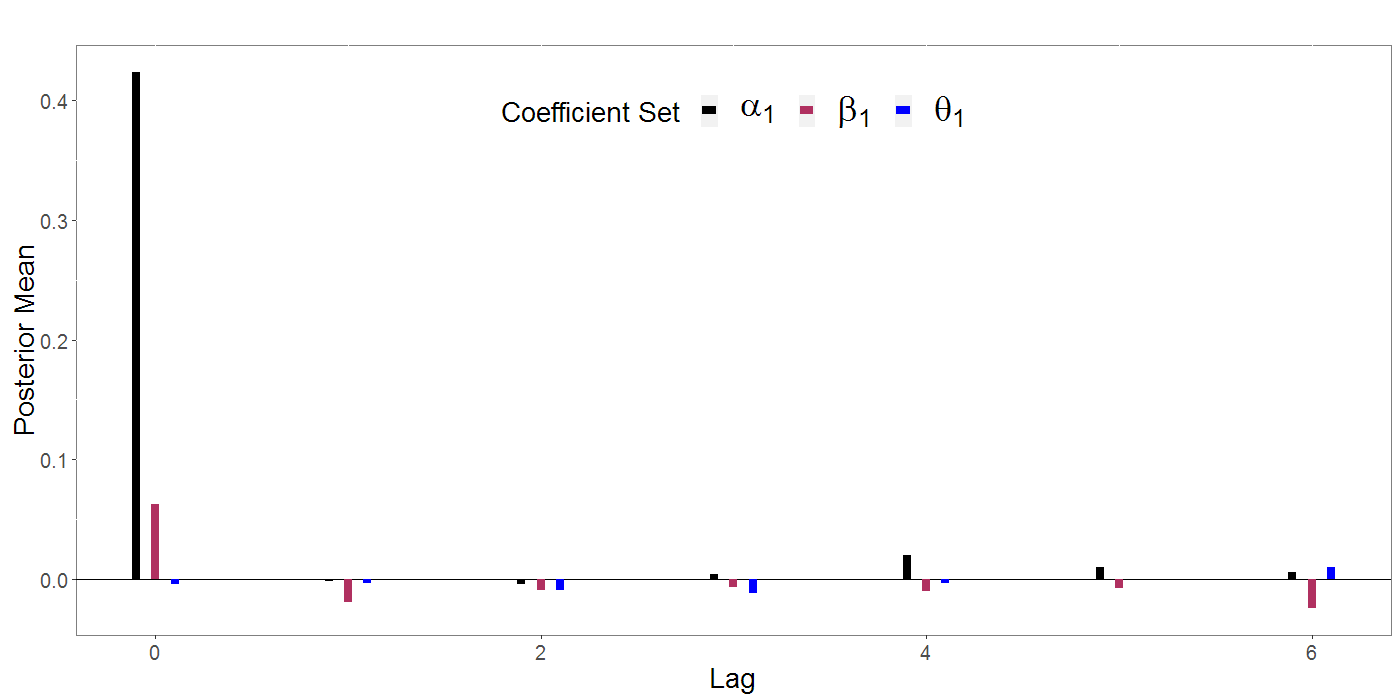
\includegraphics[scale=0.3]{GuadianaL}
\end{minipage} \hspace{\textwidth}
\begin{minipage}[h]{\textwidth}
\caption{High Regime Coefficients for Guadiana from $N_1(7)$}
\label{fig:gua2}
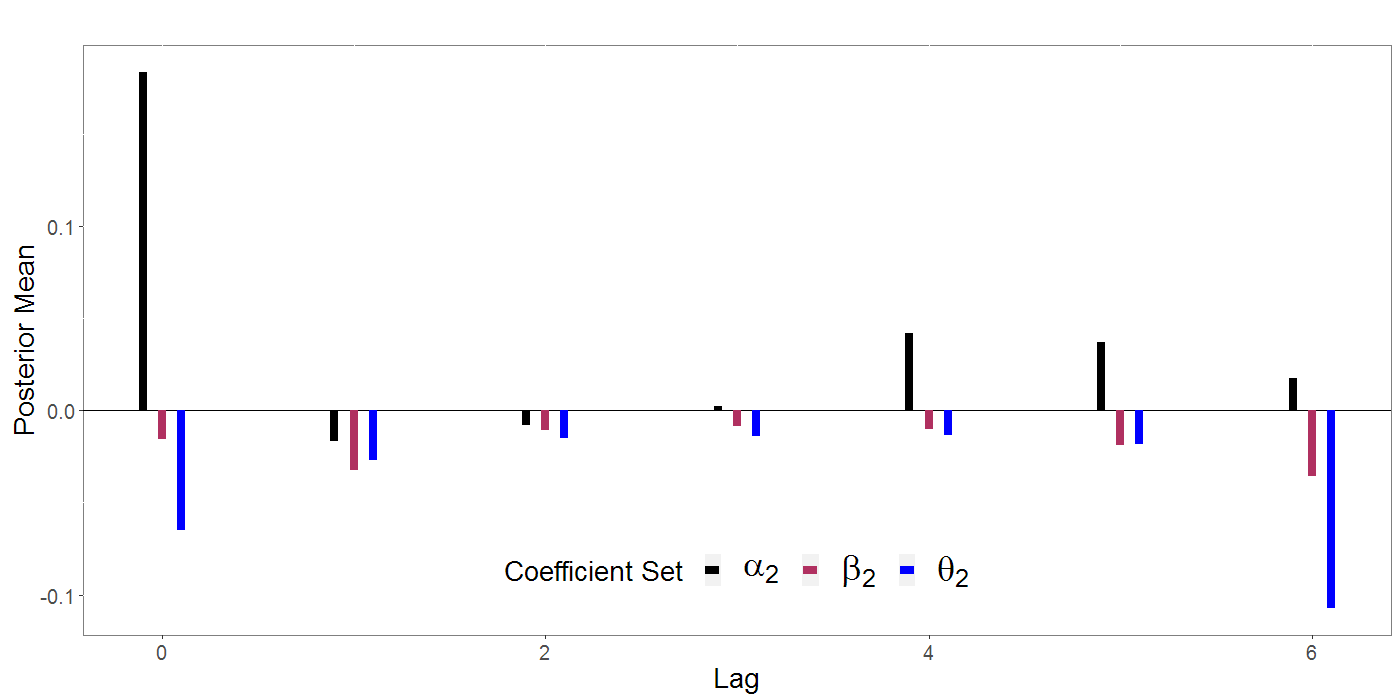
\includegraphics[scale=0.3]{GuadianaH}
\end{minipage}
\end{figure}


The next two examples involve the Jarama River where nonlinear models provided superior performance. For $h=3$, $N_2(3)$ reduced $RMSFE(3)$ by  $0.165 \textrm{ }^o C$; and for $h=7$, $N_1(7)$ reduced $RMSFE(7)$ by $0.105 \textrm{ }^o C$. Posterior expectations of $\bm{\alpha}$, $\bm{\beta}$, and $\bm{\theta}$ for $N_2(3)$ are shown in Figures \ref{fig:jar3}-\ref{fig:jar4} and for $N_1(7)$ are depicted in Figures \ref{fig:jar1}-\ref{fig:jar2}. For Jarama, it is intriguing that the optimal nonlinear model differs for the two horizons. The threshold variable in $N_2(3)$ places its largest weight of $0.66$ on $W_{t-6}$, representing information one week prior. These nonlinear models change dynamics around different thresholds: for $N_2(3)$, regime switching occurs when maximum water temperature at time $t$ surpasses its seasonal average at time $t$ by $1.20 \textrm{ }^o C$; and for $N_1(7)$, this change occurs for $0.65 \textrm{ }^o C$. The nonlinear dynamics exhibited in the low and high regimes also change with the horizon $h$. When forecasting $W_{t+3}$, the realization $W_t$ provides the most information when in the low regime; but in the high regime, none of the known information up to time $t$ is helpful. The model for forecasting $W_{t+7}$ is even more interesting since the AR dynamics in both regimes are similar to the high regime of $N_2(3)$. Knowing information at time $t$, specifically $W_t$, is only helpful in determining when to jump between means $\mu_L=0.002$ and $\mu_H=0.03$ to forecast 7-steps ahead. Obvious differences between these two horizon-specific models illustrate that for longer horizons, currently known data provide less useful information in forecasting.

\begin{figure}[!h]
\center
\begin{minipage}[h]{\textwidth}
\caption{Low Regime Coefficients for Jarama from $N_1(3)$}
\label{fig:jar3}
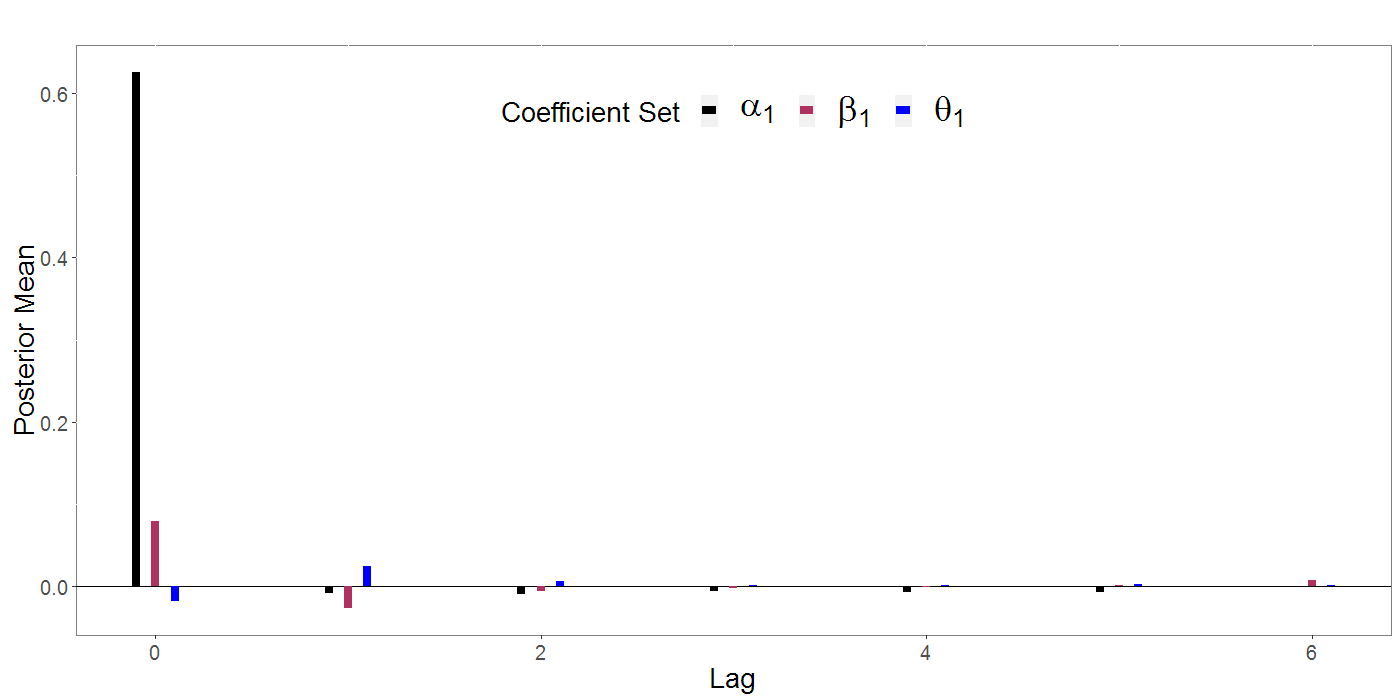
\includegraphics[scale=0.3]{JaramaL3}
\end{minipage} \hspace{\textwidth}
\begin{minipage}[h]{\textwidth}
\caption{High Regime Coefficients for Jarama from $N_1(3)$}
\label{fig:jar4}
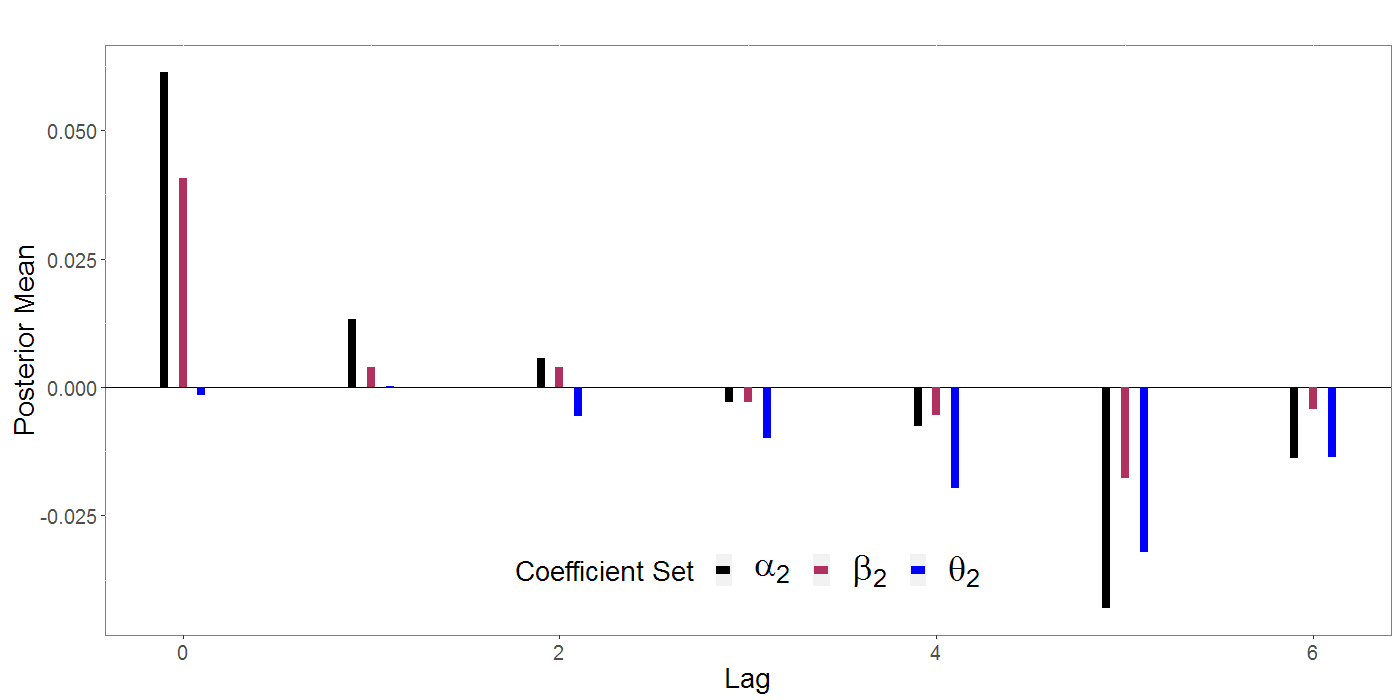
\includegraphics[scale=0.3]{JaramaH3}
\end{minipage}
\end{figure}

\begin{figure}[!h]
\center
\begin{minipage}[h]{\textwidth}
\caption{Low Regime Coefficients for Jarama from $N_1(7)$}
\label{fig:jar1}
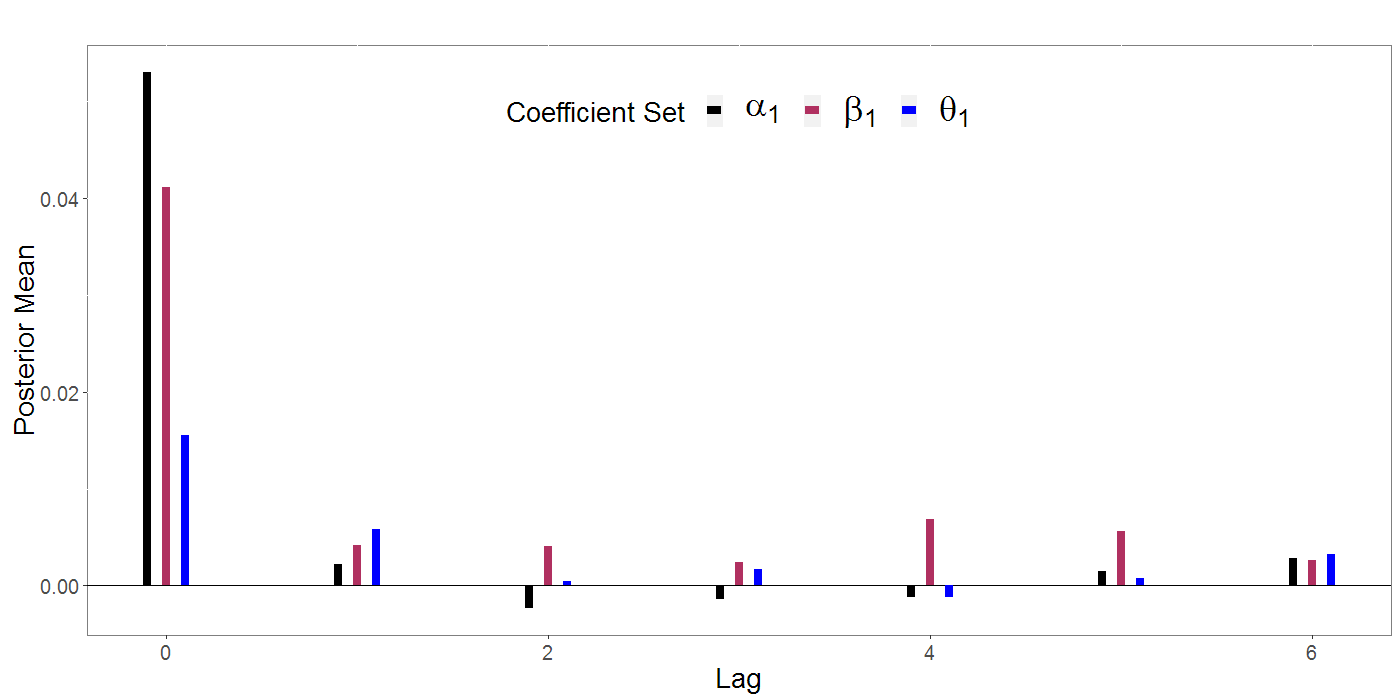
\includegraphics[scale=0.3]{JaramaL}
\end{minipage} \hspace{\textwidth}
\begin{minipage}[h]{\textwidth}
\caption{High Regime Coefficients for Jarama from $N_1(7)$}
\label{fig:jar2}
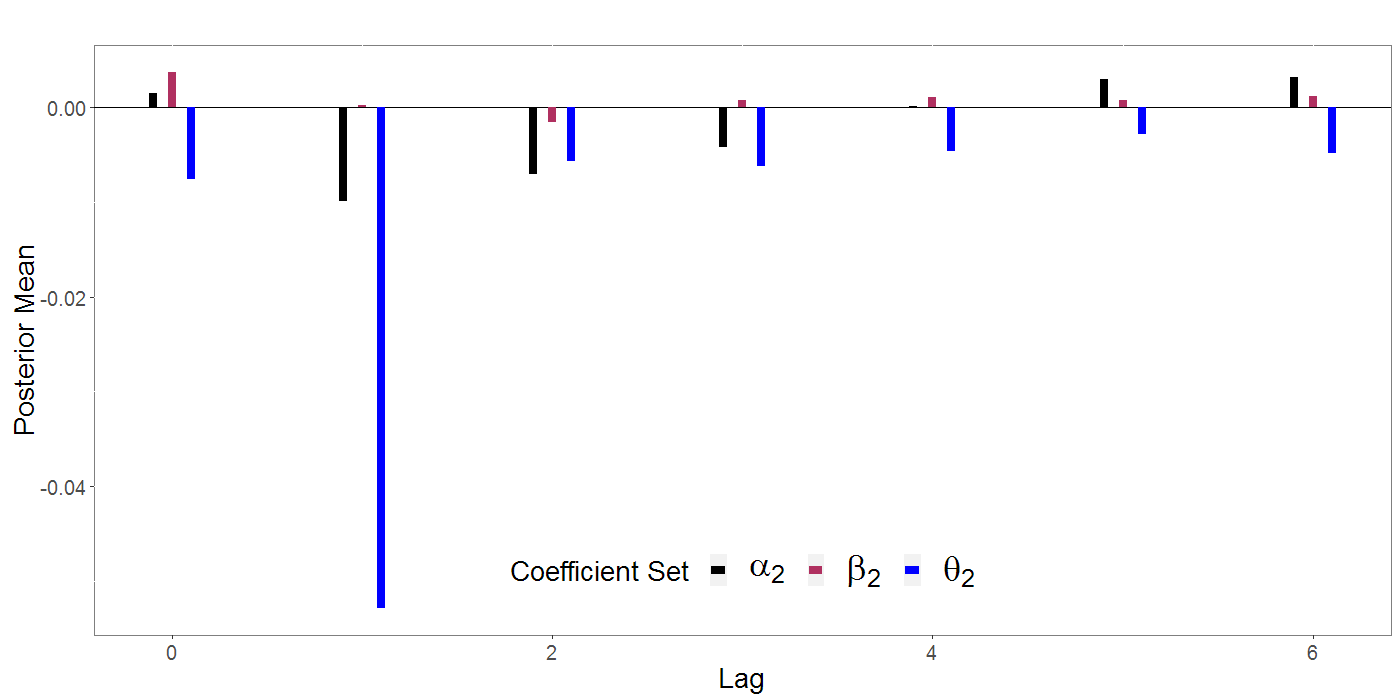
\includegraphics[scale=0.3]{JaramaH}
\end{minipage}
\end{figure}

\section{Conclusion}

Bayesian shrinkage priors for the AR coefficients and the \textit{Dirichlet} prior for a composite threshold variable are employed to estimate a flexible specification that nests the classic LSTAR model. Although simulation experiments show \textit{Dirichlet} priors to be an adequate alternative for estimating composite threshold variables, improved forecasting performance is not guaranteed. An advantage of the proposed methods is that practitioners can immediately apply them using common statistical software. Detailed code is provided with this paper for a tutorial in using Bayesian horseshoe to estimate nonlinear LSTAR models.

Recent alternatives to BLASSO and BHS based on the \textit{double-Pareto} \citep{Armagan2013} and \textit{Dirichlet-Laplace} priors \citep{Bhattacharya2015} may also be employed to estimate regime-specific autoregressive terms. Besides the jump from a linear to nonlinear LSTAR, which more than doubles the number of estimated parameters, increasing the assumed autoregressive orders in the regimes and the compositional threshold variable, further expands the parameter space causing slower convergence. For these reasons, a modified horseshoe representation is recommended for extremely sparse signals \citep{Bhadra2016}. 

The proposed methods can be easily employed to estimate nonlinear models represented by Equation \ref{eq:1} such as ESTAR and TAR. Future work involves applying and evaluating these methods on multiple regime smooth transition autoregressions (MR-STAR) where the number of unknown parameters may increase dramatically. For MR-STAR, Bayesian shrinkage may be used to circumvent the necessity for nested RJMCMC routines for each regime, or restrictive prior assumptions.

Sample code for this paper is provided in Appendix \ref{appendix1}. Code provides tutorial for implementing Bayesian regime-specific shrinkage estimation for nonlinear LSTAR models. Examples are provided in terms of a simulation study and an applied situation involving the monthly international sunspot numbers. The simulation study involving the composite threshold variable is used to illustrate the applicability and ease of the \textit{Dirichlet} prior. Code also pertaining to multistep ahead forecasts using the bootstrap method can prove to be useful in countless other situations outside the scope of this paper.


\chapter{BAYESIAN ESTIMATION OF SUBSET THRESHOLD AUTOREGRESSIVE MODELS FOR SHORT-TERM FORECASTING OF TRAFFIC OCCUPANCY}
\label{chap:traffic}
%%%%%%%%%%%%%%%%%%%%%%%%%%%%%%%%%%%%%%%%%%%%%%%%%%%%%%%%%%%%%%%%%%%%%%%
\section{Introduction}
Rising populations in major cities add stress to advanced traffic management systems (ATMS) tasked with monitoring real-time traffic variables to proactively reduce congestion. Ever since \cite{Ahmed1979} used basic ARIMA strategies to model freeway traffic networks in large US cities -- Los Angeles, Minneapolis, and Detroit -- significant research has accumulated to appropriately utilize the massive amount of data obtained in transportation networks. The global concern has manifested through independent research in major cities in places such as the United Kingdom \citep{Queen2009,Dunne2012}, Greece \citep{Stathopoulos2003, Kamarianakis2012,Theofilatos2017}, Italy \citep{Annunziato2013,Moretti2015}, China \citep{Shang2006,Jun2007,Min2010}, and Ethiopia \citep{Hellendoorn2011}. Technological advances over this time period have not only improved the gathering of the data but also in the quick distribution of pertinent information to drivers. The speed and accuracy between the detection to the correction rely on efficient modeling and accurate short-term forecasting of important traffic characteristics.

Three traffic variables have been used to quantify traffic congestion per unit of time: flow (volume per time), speed (distance per time), and occupancy (percent of time occupied) \cite{Hall1992}. \cite{Smith1997} provide insight into the state of traffic modeling 20 years ago while \cite{Vlahogianni2014} do an excellent job summarizing recent advancements in short-term traffic forecasting by posing 10 interesting challenges for future researchers. The scarcity of forecast procedures for traffic occupancy may stem from the instability acknowledged in \cite{Levin1980}. Traffic occupancy, the percent of time a detection zone is occupied, has been described as ``quality assessment measure'' as it quantifies how well traffic is moving through a network \citep{Klein1996}. Univariate approaches for modeling traffic occupancy are presented for the terminal goal of evaluating forecasts at multiple horizons. Section \ref{sec:trafficdata}  presents a challenging traffic dataset from a major arterial in Athens, Greece, used for empirical study.

Traffic occupancy has been used to help forecast other traffic characteristics \citep{Hazelton2004}.  In regards to modeling traffic occupancy, most researchers adapt similar methods seen for traffic flow and speed \citep{Kamarianakis2010}. Like other traffic variables, occupancy exhibits abrupt changes in mean, temporal dynamics, and volatility as traffic fluctuates between free flow and congested states. Realizations of recent traffic occupancy can assist in the characterization of these states. In Section \ref{sec:trafficmodels}, nonlinear threshold autoregressive (TAR) processes  model and forecast traffic occupancy. The parametric TAR structure, first discussed in \cite{Tong1990}, is a conditional autoregressive (AR) model dependent on states governed by traffic occupancy . The model is highly interpretable making it appealing to practitioners. For easy application, TAR models for each location are defined to be day-specific and horizon-specific. Also, a periodic linear regression model that adequately captures the seasonality exhibited in traffic data is used to produce baseline forecasts.

\cite{Ghosh2007} provide a case for the movement from classical inference to Bayesian inference in traffic models. Joint contributions from \cite{Broemeling1992,Geweke1993,Chen1995} formed the foundation of Bayesian TAR modeling. \cite{Campbell2004} applied reversible jump Markov chain Monte Carlo to select regime-specific AR orders. Subset selection of TAR via stochastic search variable selection \citep{George1993} was conducted by \citet{So2003,Chen2011}. For all the aforementioned approaches, the number of regimes must be known or assumed. In illustration, simulation, and application, TAR models are often restricted to have at most three regimes. 

\cite{Chan2015} transformed the nonlinear TAR model into a high dimensional linear regression. Multi-step procedures seek sparse solutions to identify the regimes and perform parameter estimation \citep{Chan2015,Chan2017}. The fully Bayesian approach of \cite{Pan2017} operates similarly by utilizing a sequence of binary inclusion variables to identify change points and select regimes. The fully saturated TAR model defined Section \ref{sec:trafficmodels} follows from \cite{Chan2015} with some slight modifications. 

Section \ref{sec:trafficest} proposes a fully Bayesian three step  procedure that automates selecting the regimes and sparse subset AR estimation within regimes. First, a fully saturated TAR model is estimated using Bayesian regularization implemented through a modified horseshoe prior \citep{Carvalho2009,Carvalho2010,Bhadra2016}. Next, the Kullback-Leibler (KL) divergence \citep{Kullback1951} combined with a forward selection algorithm identifies the regimes through comparing posterior predictive distributions of the linear AR model to multiple regime TAR models. Finally, given a restricted set of regimes, the same procedure is repeated to select the relevant dynamics within each of the regimes. The result is a parsimonious TAR model with a posterior predictive distribution close in KL distance to the posterior predictive distribution from the full model.

Section \ref{sec:trafficresults} provides empirical results of out-of-sample forecasting results from final TAR models with potentially many regimes. Baseline periodic seasonal regressions are used to produce baseline forecasts. Models are compared using the mean absolute scaled measure of forecast accuracy (MASFE) of \cite{Hyndman2006}. By scaling forecast errors by the mean absolute error from a horizon-specific naive random walk, models can be simultaneously be compared to each other and the naive method.






%%%%%%%%%%%%%%%%%%%%%%%%%%%%%%%%%%%%%%%%%%%%%%%%%%%%%%%%%%%%%%%%%%%%%%%
\section{Data}
\label{sec:trafficdata}

Real-time traffic data are obtained from the major Athen's arterial, Alexandras Avenue, along the westbound direction. Every 90 seconds in April 2000, traffic occupancy is captured from seven loop detectors abbreviated $L \in \{A,B,C,D,E,F,G\}$. The National Technical University of Athens is credited for the gathering of this data. The 2013 Traffic Research Board's (TRB) Annual Meeting Workshop used a larger ecompassing dataset in their TRANSportation Data FORecasting Competition (TRANSFOR). This competition was organized by the Aritificial Intelligence and Advanced Computing Applications Committee.  Many of the inherent characteristics in this dataset make short-term forecasting quite challenging. The winning methodology applied adaptive lasso to high-dimensional nonlinear space-time models \citep{Kamarianakis2012}. Figure \ref{fig:trafficdatamap} was created using Google Maps to provide a visual depiction of this small network with arrows representing direction of traffic flow. Loop detectors $A$, $B$, $C$, and $D$ measure traffic occupancy in the westbound direction, and detectors $E$, $F$, and $G$, in the eastbound direction.

\begin{figure}[htbp]
\caption{Locations of Loop Detectors Along Alexandras Ave. in Athens, Greece: Arrows Indicate Direction of Traffic Flow}
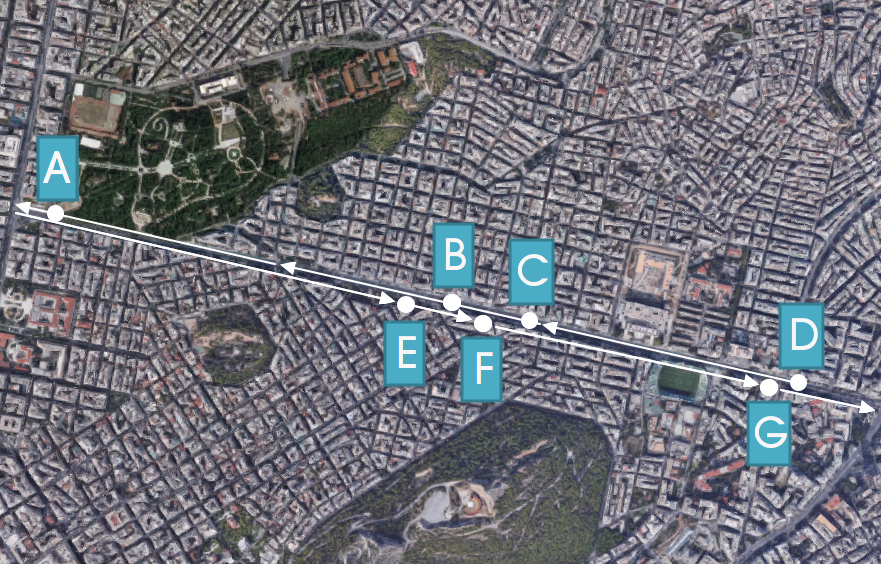
\includegraphics[width=\textwidth]{TrafficMap2}
\label{fig:trafficdatamap}
\end{figure}

Analyzing the raw traffic occupancy from an urban network measured on the 90s interval becomes problematic due to the large amount of noise seen at high resolutions \citep{Vlahogianni2014}. Temporal aggregation to larger intervals i.e. 15 min has been practiced over the years as a smoothing technique prior to modeling. Not only does this practice make short-term forecasting irrelevant with today's technology but diminishes useful long memory, nonlinear, and heteroskedastic dynamics in the underlying signal \cite{Vlahogianni2011}.Rather than modeling across different levels of temporal aggregation, as seen in \cite{Shang2006}, traffic occupancy is averaged to 3 minute intervals resulting in 480 daily time points per location. 

Define random variable $O_{L,t}$ as the traffic occupancy for location $L$ at time $t$ and $o_{L,t}$ represents a known realization. As common practice, weekend data is ignored. Cyclical human behavior patterns throughout the work week lead to weekly seasonal traffic patterns. Data during April 2000 covers four complete weeks. The first three weeks are used to fit TAR models, and the last week is designated for forecasting evaluation. Time series plots of $\{o_{L,t}\}$ are found in Figure \ref{fig:OrigPlotTrafficOcc} organized by location.

\begin{figure}[htbp]
\caption{Raw Traffic Occupancy for All Locations Measured on 3-Minute Interval: Shaded Region Indicates the Forecasting Period}
\includegraphics[width=\textwidth]{rawplots}
\label{fig:OrigPlotTrafficOcc}
\end{figure}







%%%%%%%%%%%%%%%%%%%%%%%%%%%%%%%%%%%%%%%%%%%%%%%%%%%%%%%%%%%%%
\section{Threshold Autoregressive Model}
\label{sec:trafficmodels}

\subsection{General Modeling Information}
For each location $L\in \{A,B,C,D,E,F,G\}$, day of the week $D\in\{M,T,W,Th,F\}$, and horizon $h \in \{1,3,5\}$ ,  $(L,D,h)$-specific TAR models are built to forecast $\widehat{O}_{L,t}=E[O_{L,t}|\mathcal{I}_t]$ where $\mathcal{I}_t=\{o_{L,k}\}_{k=t-h}^{t-h-P+1}$. Chosen horizons correspond to 3 min, 9 min, and 15 min ahead forecasts. The weekly periodicity of traffic occupancy modeled in \cite{Williams1999,Ghosh2007,Kamarianakis2010} and visually seen in Figure \ref{fig:OrigPlotTrafficOcc} defends $D$-specific modeling. The purpose of $h$-specific models is to ensure multi-step forecasting is user-friendly and computationally efficient for practitioners. 

The order parameter $P\in\mathbb{N}$ represents the maximum short-term lag relevant for forecasting and should be chosen large enough to cover relevant temporal dependencies across all traffic states. The order $P=7$ is fixed equating to the last 21 minutes of known information. To produce short-term forecasts, only short-term dynamics are considered. Long-term or seasonal dynamics can be included but require more periods to adequately estimate. Periodic regression models with Fourier terms adequately capture weekly seasonality and are used to produce baseline forecasts \citep{Kamarianakis2010}. As $h\to\infty$, $(L,D)$-specific seasonal models are expected to dominate over $(L,D,h)$-specific TAR models.
 
\subsection{Transformed Occupancy}
Using function $\textrm{logit}(x):(0,1)\to\mathbb{R}$ such that $\phi(x)=\log [x/(1-x)]$, define the new transformed variable $Y_{L,t}=\textrm{logit}(O_{L,t})$. Raw occupancy is bounded on the $[0,1]$ interval. Recoding $0$ with $0.0001$ and $1$ with $0.9999$ is a nonevasive technique to handle extreme occupancies when $\textrm{logit}(.)$ is undefined. All models are defined for the variable $Y_{L,t}$, an approach used for proportional time series since \cite{Wallis1987}. Figure \ref{fig:TransPlotTrafficOcc} displays the transformed series $\{y_{L,t}\}$ for each location. Although forecasts are produced for the final week, evaluation of forecasts are considered on the original scale using $\textrm{logit}^{-1}(x):\mathbb{R}\to(0,1)$ where $\textrm{logit}^{-1}(x)=\frac{\exp(x)}{1+\exp(x)}$. Since $\textrm{logit}(x)$ is a nonlinear transformation, the forecast $\hat{O}_{L,t} \neq  \textrm{logit}^{-1}(\hat{Y}_{L,t})$. Unbiased forecasts and quantiles are produced from the set $\{\textrm{logit}^{-1}(\hat{Y}^{(s)}_{L,t})\}_{s=1}^{S}$ where $\{\hat{Y}^{(s)}_{L,t}\}_{s=1}^{S}$ are $S$ posterior samples obtained from the posterior predictive distribution $f(\hat{Y}_{L,t}|\mathcal{I}^*_t)$ where $\mathcal{I}^*_t=\{y_{L,k}\}_{k=t-h}^{t-h-P+1}$.
\begin{figure}[htbp]
\caption{Logit Transformed Traffic Occupancy for All Locations Measured on 3-Minute Interval: Shaded Region Indicates the Forecasting Period}
\includegraphics[width=\textwidth]{Transplots}
\label{fig:TransPlotTrafficOcc}
\end{figure}

\subsection{General $(L,D,h)$-Specific TAR Model}
The random process $\{Y_t\}$ follows TAR model of order $P$ with $m+1$ regimes if 
\begin{equation}
\label{eq:generalTAR}
Y_{t}=\phi_0^{(j)}+\sum\limits_{i=1}^P \phi^{(j)}_i Y_{t-h-i+1}+\sigma\epsilon_{t}, \textrm{ for } \delta_{j-1}<Y_{t-h}\leq \delta_{j},
\end{equation}
where $\sigma>0$, $j\in\{1,2,\cdots,m+1\}$, and $h \in \mathbbm{N}$. The vector of thresholds $\bm{\delta}=[\delta_1,\delta_2,\cdots,\delta_m]'$ divides the process into $m+1$ regimes where $-\infty=\delta_0<\delta_1\leq\delta_2\leq \cdots \leq \delta_m<\delta_{m+1}=\infty$. Since the most recent realization $Y_{t-h}$ determines the current model state, the TAR model is conventionally classified as ``self-exciting" \citep{Ghaddar1981}. The sequence of errors $\{\epsilon_t\}$ are assumed to be i.i.d. with zero mean and unit variance.

The TAR structure in Equation \ref{eq:generalTAR} is slightly more rigid than the classic structure in \cite{Chen1995}. Rather than utilizing regime-specific variance parameters $\sigma_j$,  homoskedasticity is assumed. When $\textrm{logit}^{-1}(x)$ is used to obtain density forecasts on the original $[0,1]$ scale, heteroskedasticity is naturally captured. This is analogous to \textit{Beta} distributed random variables where the variance is dependent on the mean. Another key difference arises in the selection of the transition variable. Often a delay parameter $d$ is introduced and $Y_{t-d}$ drives regime changes. Following from \cite{Chan2015}, $d$ is known and  $d=h$ is fixed. Exogenous traffic variables nor time are considered for the transition variable.

\subsection{High Dimensional Linear Representation}
To reformulate Equation \ref{eq:generalTAR} into a high dimensional linear regression model, a slight deviation from the procedure in \cite{Chan2015,Chan2017} is outlined with similar notation for consistency. Suppose the discrete time series $\{y_t\}_{t=1-h-P+1}^T$ is observed. Let $\bm{y}=[y_{1},\cdots,y_{T}]'$, $\bm{\epsilon}=[\epsilon_{1},\cdots,\epsilon_{T}]'$, and define matrix $\bm{X}$ by
$$
\bm{X}=\begin{bmatrix}
    1 & y_{1-h} & y_{1-h-1} & \dots  & y_{1-h-P+1} \\
    1 & y_{2-h} & y_{2-h-1} & \dots  & y_{2-h-P+1} \\
    \vdots & \vdots & \vdots & \ddots & \vdots \\
    1 & y_{T-h} & y_{T-h-1} & \dots  & y_{T-h-P+1}
\end{bmatrix}.
$$
The $T\times 1$ response vector $\bm{y}$, $T\times 1$ error vector $\bm{\epsilon}$, and  $T \times (1+P)$ model matrix $\bm{X}$ are often seen in matrix representations of $h$-specific AR$(P)$ models.

The second column in $\bm{X}$ contains the sequence of $h$-specific transition variables. Define the sorting function $\pi(i):\{1,\cdots,T\}\to\{1,\cdots,T\}$   where $\pi(i)$ equates to the time index of the $i$th smallest element in $[y_{1-h},y_{2-h},\cdots,y_{T-h}]'$. The new $\bm{y}_R=[y_{\pi(1)+h},\cdots,y_{\pi(T)+h}]'$, $\bm{\epsilon}_R=[\epsilon_{\pi(1)+h},\cdots,\epsilon_{\pi(T)+h}]'$ and 
$$
\bm{X}_1=\begin{bmatrix}
    1 & y_{\pi(1)} & y_{\pi(1)-1} & \dots  & y_{\pi(1)-P+1} \\
    1 & y_{\pi(2)} & y_{\pi(2)-1} & \dots  & y_{\pi(2)-P+1} \\
    \vdots & \vdots & \vdots & \ddots & \vdots \\
    1 & y_{\pi(T)} & y_{\pi(T)-1} & \dots  & y_{\pi(T)-P+1}
\end{bmatrix}=
\begin{bmatrix}
\bm{y}'_{\pi(1)} \\
\bm{y}'_{\pi(2)} \\
\vdots \\
\bm{y}'_{\pi(T)} \\
\end{bmatrix}
$$
are essentially $\bm{y}$, $\bm{\epsilon}$, and $\bm{X}$ sorted according to the order statistics of the transition variable. The reordered errors in $\bm{\epsilon}_R$ are assumed to be i.i.d. with mean $0$ and variance $\sigma^2$.

In practical application, it makes sense to limit the TAR model to $m+1$ regimes requiring the estimation of $m$ thresholds in the range of the transition variable. Let $q(.): [0,1]\to[\min\{y_{t-h}:t=1,2,\cdots,T\},\max\{y_{t-h}:t=1,2,\cdots,T\}]$ denote the sample quantile function and consider a sequence $\{p_k\}_{k=1}^m$ of $m$ evenly spaced percentiles such that $p_{min}=p_1<\cdots<p_m=p_{max}$. For a fully saturated TAR model limited to $(m+1)$ regimes, fix \textit{a priori} the vector of thresholds $\bm{\delta}=[q(p_{1}),q(p_2),\cdots,q(p_{m})]'$. For $j \in \{2,\cdots,m+1\}$, let $k_j$ represent the number of elements in $[y_{1-h},y_{2-h},\cdots,y_{T-h}]'$ less than $q(p_{j-1})$ and  define 
$$\bm{X}_j=
\begin{bmatrix}
    0 & 0 & 0 & \dots  & 0 \\
    \vdots & \vdots & \vdots & \ddots & \vdots \\
    0 & 0 & 0 & \dots  & 0 \\
    1 & y_{\pi(k_j+1)} & y_{\pi(k_j+1)-1} & \dots  & y_{\pi(k_j+1)-P+1} \\
    \vdots & \vdots & \vdots & \ddots & \vdots \\
    1 & y_{\pi(T)} & y_{\pi(T)-1} & \dots  & y_{\pi(T)-P+1}
\end{bmatrix}=
\begin{bmatrix}
0 \\
\vdots \\
0\\
\bm{y}'_{\pi(k_j+1)} \\
\vdots \\
\bm{y}'_{\pi(T)} \\
\end{bmatrix}.
$$

Finally, a slightly restricted version of the $(m+1)$-regime TAR process seen in Equation \ref{eq:generalTAR} can be expressed as a linear regression by
\begin{equation}
\label{eq:hdlinmod}
\begin{split}
\bm{y}_R &=\bm{X}_R\bm{\theta}_R+\bm{\epsilon}_R \\
\end{split}
\end{equation}
where $\bm{X}_R=[\bm{X}_1,\bm{X}_2,\cdots,\bm{X}_{m+1}]$ is a $T\times (P+1)(m+1)$ model matrix and $\bm{\theta}_R=[\bm{\theta}'_{1},\bm{\theta}'_2,\cdots,\bm{\theta}'_{m+1}]'$ is a $(P+1)(m+1) \times 1$ vector of coefficients grouped by regime. From Equation \ref{eq:generalTAR}, set $\bm{\phi}_j=[\phi^{(j)}_0,\phi^{(j)}_1,\cdots,\phi^{(j)}_P]'$. Starting with $\bm{\theta}_1=\bm{\phi}_1$, the state dependent coefficient group $\bm{\theta}_j=\bm{\phi}_{j}-\bm{\phi}_{j-1}$ for $j \in \{2,\cdots,m+1\}$ represents the marginal adjustment in dynamics when $y_{t-h}$ crosses the threshold $\delta_{j-1}=q(p_{j-1})$.

\subsection{Baseline Seasonal Model}
Seasonal models allow us to understand the long-run relationship of a variable over time through repetitive cycles. It is common practice in time series analysis to deseasonalize data prior to model buiding through smoothing or seasonal differencing. In many studies, seasonal autoregressive integrated moving average models (SARIMA) have been used to analyze traffic characteristics \citep{Williams2003, Ghosh2005, Zhang2011}. As detailed in \cite{Kumar2015}, these models require large databases of historical data to capture seasonal phenomenon. Similar to \cite{Kumar2015}, a 3 day period is used for model training. From a similar dataset, \cite{Kamarianakis2010} used a smoothing spline with 150 degrees of freedom to magnify weekly seasonal patterns and identify structural changes. Smoothing approaches can lead to simple models that can forecast at all horizons.

Harmonic regressions estimate daily periodic signals from a linear regression over a Fourier basis \citep{Metcalfe2009}. For 3-min data, the seasonal period has a length of 480 discrete measures. Using harmonic regression, $(L,D)$-specific seasonal profiles of $\{Y_t\}$ are fitted. Expressed in Equation \ref{eq:trafficseas}, the harmonic seasonal model is restricted to the first $H$ terms of the Fourier series.  This model is not considered a baseline model for its simplicity in estimation but for its simplicity in multi-step forecasting at all horizons. The error $\{\epsilon_t\}$ are assumed i.i.d. with mean 0 and unit variance.
\begin{equation}
\label{eq:trafficseas}
Y_{t}=\mu+\sum\limits_{j=1}^{H} \Big[\alpha_{j}\sin\Big(\frac{2\pi tj}{480}\Big)+\beta_{j}\cos\Big(\frac{2\pi tj}{480}\Big)\Big]+\sigma\epsilon_{t}
\end{equation}

Fitting the model in Equation \ref{eq:trafficseas} is not difficult since it can also be represented as a high dimensional linear regression model like
\begin{equation}
\label{eq:hdslinmod}
\begin{split}
\bm{y}_F &=\bm{X}_F\bm{\theta}_F+\bm{\epsilon}_F \\
\end{split}
\end{equation}
where $\bm{y}_F=[y_1,y_2,\cdots,y_T]'$, $\bm{\epsilon}_F=[y_1,y_2,\cdots,\epsilon_T]'$, and $\bm{\theta}_F=[\mu,\alpha_1,\cdots,\alpha_H,\beta_1,\cdots,\beta_H]'$. The model matrix  $\bm{X}_F=[\bm{1},\bm{SIN},\bm{COS}]$ where $\bm{1}$ is a $T\times 1$ vector of $1$s, $\bm{SIN}$ is a $T\times H$ matrix containing the Fourier sine terms, and $\bm{COS}$ is a $T\times H$ matrix containing the Fourier cosine terms.

\subsection{Special Considerations for Traffic Modeling}
The linear matrix form of TAR in Equation \ref{eq:hdlinmod} arises from restricting the set of possible thresholds  $\bm{\delta}$ to a finite set of quantiles based on the sampled transition variable. The high dimensional regression model in \cite{Chan2015,Chan2017} represents a fully saturated TAR model where every realization in the series $\{y_t\}_{t=1}^T$ resides in a different regime. In classic Bayesian handling of TAR and the related smooth transition autoregressive model (STAR), the number of regimes, $(m+1)$, is fixed. To restrict estimation of the $m$ thresholds to the range of $Y_{t-h}$, slightly informative \textit{uniform} priors bounded by empirical quantiles $q(p_{min})$ and $q(p_{max})$ ensure that at least $(1-\min\{p_{min},1-p_{max}\})\times 100\%$ of the data is represented in the lowest and highest regime \citep{Chen1995,Chen1998,Lubrano2000,Lopes2006}. Following from literature, $p_{min}=0.15$ and $p_{max}=0.85$ are selected to slightly reduce the dimensionality of $\bm{X}$.

For $(L,D,h)$-specific traffic models, the maximum number of thresholds is fixed to $m=50$ and the maximum autoregressive order to $P=7$. The model matrix $\bm{X}_R$ of the fully saturated $51$-regime TAR$(7)$ has dimension $T^*\times 408$. The fitting period for each model contains $T=1440$ discrete time realizations of $\{Y_t\}$ leading to $T^*=1440-h-7+1 > 408$. The predetermined threshold vector $\bm{\delta}=[q(0.15),q(p_2),\cdots,q(p_{49}),q(0.85)]'$ constructed from $m$ evenly spaced percentiles ensures approximately $\frac{0.85-0.15}{50}=0.014$ of the full time series is represented in each potentially relevant regime. These modifications to the framework of \cite{Chan2015,Chan2017} are made to ensure the dimensionality of the parameter space is not unnecessarily large for practical application. Based on this approach, it is recommended to select $m$ large enough to ensure the set of quantile-based thresholds is dense to not reduce error in misspecified \textit{a priori} selection of $\bm{\delta}$.

For $(L,D)$-specific seasonal models, the number of Fourier sine/cosine pairs $H$ must be less than half the period. Regularized estimation of these models using adaptive LASSO \citep{Zou2006} indicated that the largest significant harmonic of the model in Equation \ref{eq:trafficseas} across locations and days was for $j=139$. Before estimating these seasonal profiles under the Bayesian framework, a maximum number of harmonics, $H=150$, is chosen. The vector of coefficients $\bm{\theta}_F$ contains $2H+1=301<1440=T$ parameters that require estimation. To ensure weekly periodic signals are smooth, sparse estimation of $\bm{\theta}_F$ is desired.








%%%%%%%%%%%%%%%%%%%%%%%%%%%%%%%%%%%%%%%%%%%%%%%%%%%%%%%%%%%%
\section{Bayesian Estimation, Regime Identification, and Subset Selection}
\label{sec:trafficest}

The purpose of representing the $(m+1)$-regime TAR process as a high dimensional linear regression is to make Bayesian posterior estimation and model selection computationally feasible for multiple regime TAR models. More importantly, the fully saturated regression $\bm{y}_R=\bm{X}_R\bm{\theta}_R+\bm{\epsilon}_R$ nests a finite, but extensive, library of $(m^*+1)$-regime subset TAR$(P)$ models where $0\leq m^*\leq m$. This includes all linear subset AR$(P)$ models.

For simplicity, let $\bm{\Theta}=[\bm{\theta}'_R,\sigma^2]'=[\bm{\theta}'_1,\cdots,\bm{\theta}'_{m+1},\sigma^2]'$. It is believed that the optimal choice $m^*$ is small implying that only $m^*+1$ of the vectors in $\{\bm{\theta}'_1,\bm{\theta}'_2,\cdots,\bm{\theta}'_{m+1}\}$ are nonzero implying that $\bm{\theta}_R$ is sparse. To simultaneously estimate $\bm{\theta}_R$, choose the optimal $m^*$, and identify the thresholds, \cite{Chan2015} recommends using the penalized group LASSO estimate $\hat{\bm{\theta}}_{GL}$ of \cite{Yuan2006} seen in Equation \ref{eq:grouplasso}. The parameter $\lambda$ controls regularization, $||\cdot||_2$ is the $\ell_2$-norm, and $||\cdot||_1$ is the $\ell_1$-norm.
\begin{equation}
\label{eq:grouplasso}
\hat{\bm{\theta}}_{GL}=\underset{\bm{\theta}_R}{\textrm{argmin}}=\frac{1}{T}||\bm{y}_R-\bm{X}\bm{\theta}_{R}||_2^2+\lambda\sum\limits_{j=1}^{m+1}||\bm{\theta}_j||_1
\end{equation}

When $\bm{X}_R$ is constructed as seen in \cite{Chan2015},the set of thresholds identified from $\hat{\bm{\theta}}_{GL}$ consistently estimates the true thresholds if the true $m^*$ is known \textit{a priori}. In practice, $m^*$ is unknown, and $\hat{\bm{\theta}}_{GL}$ overestimates the number of regimes. Second stage selection of the best subset of the group LASSO identified thresholds via penalized information criteria (IC), i.e. AIC \citep{Li2012}, BIC \citep{Yao1988}, or MDL \citep{Davis2006}, leads to consistent estimation of the true set of thresholds \citep{Chan2015}. The three-step procedure of \cite{Chan2017}, primarily based on a group orthogonal greedy algorithm (GOGA) and high dimensional information criteria (HDIC), significantly outperforms two-step group LASSO approach in \cite{Chan2015}.

The estimation procedures of \cite{Chan2015,Chan2017} focus on estimation and selection of $\bm{\delta}$ assuming $P$ is known and the same for each regime. The consistency and convergent rate maintain when these assumptions are dropped. Using the Bayesian framework, a three step procedure, outlined in Sections \ref{sec:stage1}, \ref{sec:stage2}, and \ref{sec:stage3}, identifies the important regimes with potentially subset AR$(P)$ dynamics. The order parameter $P$ should be chosen large enough to cover all temporal dynamics across all regimes, and, as previously mentioned, $P=7$ for all $(L,D,h)$-specific traffic occupancy subset TAR$(P)$ models.

\subsection{Bayesian Penalized Estimation}
\label{sec:stage1}

\subsubsection{Conditional Likelihood}
All Bayesian inference extends from the full posterior distribution $p(\bm{\Theta}|\bm{y}_R,\bm{X}_R)$. As Bayes' rule suggests, the full posterior distribution is expressed as
\begin{equation}
\label{eq:fullpost}
p(\bm{\Theta}|\bm{y}_R,\bm{X}_R) \propto p(\bm{y}_R|\bm{X}_R,\bm{\Theta})p(\bm{\Theta})
\end{equation}
where $p(\bm{y}_R|\bm{X}_R,\bm{\Theta})$ is the model likelihood and $p(\bm{\Theta})$ is the prior. Options for $p(\bm{\Theta})$ are discussed in the subsequent section, but all immediate attention is on the model likelihood $p(\bm{y}_R|\bm{X}_R,\bm{\Theta})$. Given the linear model $\bm{y}_R=\bm{X}_R\bm{\theta}_R+\bm{\epsilon}_R$, the likelihood $p(\bm{y}_R|\bm{X}_R,\bm{\Theta})$ stems from a distributional assumption about the errors $\{\epsilon_{\pi(t)+h}\}$ in $\bm{\epsilon}_R$. So far, we have assumed $\{\epsilon_{\pi(t)+h}\}$ are i.i.d. with mean $0$ and variance $\sigma^2$. For modeling traffic occupancy, we consider and compare two distribution options.

Assume $\{\epsilon_{\pi(t)+h}\} \sim \textrm{ i.i.d. }\mathcal{N}(0,\sigma^2)$ where $\mathcal{N}$ denotes the \textit{normal} distribution. Throughout statistics, this is the most commonly used distribution for the errors. The \textit{normal} regression model is recognized by 
\begin{equation}
\label{eq:normalmod}
\bm{y}_R|\bm{X}_R,\bm{\Theta}\sim \mathcal{N}_T(\bm{X}_R\bm{\theta}_R,\sigma^2\bm{I})
\end{equation}
where $\mathcal{N}_T$ is a $T$-dimensional \textit{Multivariate normal} distribution and $\bm{I}$ is a $T\times T$ identity matrix. The \textit{Guassian} error specification for all $(L,D,h)$-specific TAR models and $(L,D)$-specific seasonal harmonic profiles is used with caution. Even after aggregating to a 3-min interval, influential spikes toward $0$ and $1$ are seen. For future reference, we let TAR and SEAS denote the \textit{normal} regression models from Equations \ref{eq:hdlinmod} and \ref{eq:hdslinmod}. In both TAR and SEAS, Jefferys' prior is used for $\sigma^2$. Derivation of the \textit{inverse-gamma} full conditional distribution for $\sigma^2$ under both linear models can be found in \cite{bayesreg}.

\subsubsection{Horseshoe+ Priors for Penalized Regression}

\cite{Mallick2013} examines the historical significance of Bayesian model selection approaches in high dimensional linear models. Bayesian penalized regression methods using continuous scale-mixture priors \citep{OHara2009,Polson2010} have been proposed to approximate the spike-and-slab shape of discrete mixture priors \citep{Mitchell1988,George1993,Madigan1994,Carlin1995,Kuo1998,Ishwaran2005,Ishwaran2011}.

Specifically, the Bayesian horseshoe (BHS) estimator of \citep{Carvalho2009,Carvalho2010} has been extensively researched and shown to have excellent theoretical properties in achieving sparsity \citep{Polson2012,Datta2013,vanderPas2014}. The BHS prior falls in the extensive class of shrinkage priors with global-local hierarchical representations \citep{Polson2010}. As common to regularization techniques, a global tuning parameter is used to enforce variable selection by shrinking coefficients toward 0. However, BHS utilizes additional coefficient-specific tuning parameters to ensure relevant effects are not overshrunk. 

The horseshoe+ estimator ($\textrm{BHS}^+$) of \cite{Bhadra2016} results from a slightly modified hierarchy with additional tuning on the local level. The $\textrm{BHS}^+$ hierarchical prior for each parameter $\theta_i$ in the full parameter vector $\bm{\theta}_R$ is represented as
\begin{equation}
\label{eq:traffichsp}
\begin{split}
	\theta_i|\lambda_i,\tau,\sigma^2 & \sim \mathcal{N}(0,\lambda^2_i\tau^2\sigma^2) \\
	\lambda_i &\sim \mathcal{C}^+(0,\eta_i)\\
	\eta_i & \sim \mathcal{C}^+(0,1)\\
	\tau &\sim \mathcal{C}^+(0,1)\\
\end{split}
\end{equation}
where $\mathcal{C}^+$ is the \textit{half-Cauchy} distribution. The $\textrm{BHS}^+$ prior provides better detection of ultra-sparse signals than the original BHS; therefore, $\textrm{BHS}^+$ shrinkage priors are preferred in all TAR and SEAS models.  Additional theoretical and empirical defense of $\textrm{BHS}^+$ priors in the high dimensional regression setting, see \cite{Bhadra2016} and Appendix \ref{appendix3}.

The original hierarchy seen in Equation \ref{eq:traffichsp} makes posterior sampling difficult since full conditional distributions are not obtainable. By exploiting the scale-mixture decomposition of the \textit{half-Cauchy} distribution using \textit{inverse gamma} distributions abbreviated $\mathcal{IG}$ \citep{Wand2011}, \cite{Makalic2016b} derived full conditional distributions for all parameters in $\bm{\Theta}$ so Gibbs sampling \citep{Geman1987,Gelfand1990} can be utilized to sample from the full posterior distribution $p(\bm{\Theta}|\bm{y}_R,\bm{X}_R)$. Equation \ref{eq:traffichsp2} reflects the changes to the $\textrm{BHS}^+$ hierarchy for each parameter $\theta_i$ in $\bm{\theta}_R$.
\begin{equation}
\label{eq:traffichsp2}
\begin{split}
\theta_i|\lambda_i^2,\tau^2,\sigma^2 & \sim \mathcal{N}(0,\lambda_i^2\tau^2\sigma^2) \\
\lambda^2_i|\nu_i & \sim \mathcal{IG}(1/2,1/\nu_i)\\
\tau^2|\xi & \sim \mathcal{IG}(1/2,1/\xi)\\
\nu_i & \sim \mathcal{IG}(1/2,1) \\
\xi & \sim \mathcal{IG}(1/2,1) \\
\end{split}
\end{equation}

\subsubsection{Posterior Sampling}
The high dimensional TAR and SEAS models, with large $\bm{X}_R$ and $\bm{X}_F$ design matrices, causes issues in Gibbs sampling. Specifically, the full conditional distributions of $\bm{\theta}_R$ and $\bm{\theta}_S$ require large $408\times 480$ and $301\times 301$ matrices, respectively. To obtain $S$ posterior samples $\{\bm{\theta}^{(s)}_R\}_{s=1}^{S}$ and $\{\bm{\theta}^{(s)}_F\}_{s=1}^{S}$, inversion of $\bm{X}'_R\bm{X}_R$ and $\bm{X}'_S\bm{X}_S$ is required in the derived \textit{multivariate normal} full conditional distributions. In all cases, the algorithm of \cite{Rue2001} provides fast Gibbs sampling, but for larger choices of $m$, $P$, and $H$, the algorithm of \cite{Bhattacharya2016} is a helpful alternative. For both TAR and SEAS models,  $S=2000$ posterior samples after a burn-in period of $5000$ and with a thinning of $10$ was large enough to ensure the minimum effective sample size of all parameters was larger than $150$. Posterior means and quantiles capture the uncertainty of the models given the data. Even though $\textrm{BHS}^+$ shrinkage priors are applied for both TAR and SEAS, posterior means of irrelevant effects in $\bm{\theta}_R$ and $\bm{\theta}_S$ will never equal 0. The profiles obtained from all SEAS models satisfactorily captured the weekly periodic signal from the first three weeks of April. For the TAR models, the three step procedure continues to identify which autoregressive groups are irrelevant, and then perform variable selection ignoring the natural grouping. Let $\mathcal{M}_R$ represent the fully saturated TAR model fitted using $\textrm{BHS}^*$. The primary goal of the next two steps is to search for the best submodel $\mathcal{M}_*$ from the $2^{(m+1)(P+1)}$ different possible submodels $\mathcal{M}_\perp$. When $m=50$ and $P=7$, there are $6.61\times 10^{122}$ subset TAR$(P)$ models. Naive exploration of this model space is not recommended.

\subsection{Regime Identification}
\label{sec:stage2}

The samples $\{\bm{\theta}^{(s)}_R\}_{s=1}^S$ and $\{\sigma^{(s)}\}_{s=1}^S$ from the joint posterior distribution $$p(\bm{\theta}_{R},\sigma^2|\mathcal{M}_R,\bm{y}_R,\bm{X}_R)$$ is a good starting point for forecasting since $\textrm{BHS}^+$ priors were used to enforce sparsity. Under model $\mathcal{M}_R$, density forecasts at time $T+1$ can be obtained from the posterior predictive distribution represented by $$p(y_{T+1}|\mathcal{M}_R,\bm{y}_R,\bm{X}_R).$$ Assuming the model $\mathcal{M}_R$ produces reasonable forecasts, it can serve as a valid reference model. Given a simpler submodel $\mathcal{M}_\perp$, the Kullback-Leibler (KL) divergence \citep{Kullback1951} measures the distance between the posterior predictive distributions \citep{Goutis1998,Dupuis2003}. If minor discrepancy is detected between $\mathcal{M}_R$  and $\mathcal{M}_\perp$, the more parsimonious model is favored. 

Samples $\{\bm{\theta}^{(s)}_\perp\}_{s=1}^S$ and $\{\sigma^{(s)}_\perp\}_{s=1}^S$ from the joint posterior distribution $$p(\bm{\theta}_\perp,\sigma^2_\perp|\mathcal{M}_\perp,\bm{y}_\perp,\bm{X}_\perp)$$ are obtained via projection removing the need for repeated Gibbs sampling. In this representation, $\bm{y}_\perp=\bm{y}_R$ and $\bm{X}_\perp$ contains the columns of $\bm{X}_R$ associated with the submodel $\mathcal{M}_\perp$. \cite{Piironen2017} derived analytical solutions to acquire the projected samples and measure the KL divergence from forecasts under $[\bm{\theta}^{'(s)}_R,\sigma^{(s)}_R]'$ versus $[\bm{\theta}^{'(s)}_\perp,\sigma^{(s)}_\perp]'$ for linear Gaussian models. The $s$th posterior sample  $[\bm{\theta}^{'(s)}_\perp,\sigma^{(s)}_\perp]'$ is given in Equation \ref{eq:trafficproj}. For each posterior draw from $p(\bm{\theta}_R,\sigma^2_R|\mathcal{M}_{R},\bm{y}_R,\bm{X}_R)$, the associated KL divergence $d_{\perp}$ is given Equation \ref{eq:trafficklds}. 
\begin{equation}
\label{eq:trafficproj}
\begin{split}
\bm{\theta}^{(s)}_\perp&=(\bm{X}'_\perp\bm{X}_\perp)^{-1} \bm{X}'_\perp \bm{X}_R\bm{\theta}^{(s)}_R\\
\sigma^{(s)}_\perp&=\sqrt{(\sigma^{(s)}_R)^2+\frac{(\bm{X}_R\bm{\theta}^{(s)}_R-\bm{X}_\perp\bm{\theta}^{(s)}_\perp)'(\bm{X}_R\bm{\theta}^{(s)}_R-\bm{X}_\perp\bm{\theta}^{(s)}_\perp)}{T}                                  }\\
\end{split}
\end{equation}

\begin{equation}
\label{eq:trafficklds}
\begin{split}
d^{(s)}_{\perp}(\bm{\theta}^{(s)}_R,\sigma^{(s)}_R)&=\frac{1}{2}\log\bigg(\frac{\sigma^{(s)}_\perp}{\sigma^{(s)}_R}\bigg)^2\\
\end{split}
\end{equation}

Finally, averaging the KL divergences across all posterior samples estimates the overall discrepancy between posterior predictive distributions of $\mathcal{M}_R$ and $\mathcal{M}_\perp$. This discrepancy, denoted $D(\mathcal{M}_{R}||\mathcal{M}_\perp)$, is expressed in Equation \ref{eq:trafficdisc}. 
\begin{equation}
\label{eq:trafficdisc}
\begin{split}
D(\mathcal{M}_{R}||\mathcal{M}_\perp)&=\frac{1}{S}\sum\limits^S_{s=1} d^{(s)}_{\perp}(\bm{\theta}^{(s)}_R,\sigma^{(s)}_R)   \\
\end{split}
\end{equation}

Using these concepts, surveying the entire model space is avoided by employing a forward stepwise selection algorithm similar to \cite{Piironen2015}. Starting with the linear AR$(P)$ model, denoted $\mathcal{M}^{(1)}_{\perp}$ where $\bm{\theta}_j=0$ if $j>1$ and $\bm{\theta}^{(1)}_\perp=[\bm{\theta}'_1,\bm{0}',\bm{0}',\cdots,\bm{0}']'$, the initial discrepancy $D(\mathcal{M}_{R}||\mathcal{M}^{(1)}_{\perp})$ represents the maximum divergence between the fully saturated $\mathcal{M}_R$ and all nested TAR$(P)$ models with less than $(m+1)$ regimes. For each $j \in \{2,\cdots,m+1\}$, $\bm{\theta}_j$ is added to $\bm{\theta}^{(1)}_\perp$ and the best $2$-regime TAR$(P)$ model $\mathcal{M}^{(2)}_\perp$ that minimizes the discrepancy in Equation \ref{eq:trafficdisc} is selected. Likewise, this procedure is continued to identify the best $3$-regime TAR$(P)$, $4$-regime TAR$(P)$, and $j$-regime models, denoted $\bm{\theta}^{(3)}_\perp$, $\bm{\theta}^{(4)}_\perp$, and $\bm{\theta}^{(j)}_\perp$, respectively. Although this process can be continued up to $j=m+1$, where 
$D(\mathcal{M}_{R}||\mathcal{M}^{(m+1)}_{\perp})=0$, a stopping rule is enforced based on relative explanatory power ($RelE$) given in Equation \ref{eq:trafficrep} \citep{Dupuis2003}. Based on the additive properties of KL, $RelE$ strictly increases from $0$ to $1$. In the traffic application, regime-specific AR$(P)$ parameter groups are added until $RelE$ exceeds $0.95$.
\begin{equation}
\label{eq:trafficrep}
\begin{split}
RelE(\mathcal{M}_\perp)&=1-\frac{D(\mathcal{M}||\mathcal{M}_\perp)}{D(\mathcal{M}||\mathcal{M}^1)}\\
\end{split}
\end{equation}


\subsection{Subset Variable Selection}
\label{sec:stage3}

Let $\mathcal{J}=\{j: \bm{\theta}_j \neq 0\}$ indicate the AR$(P)$ parameter groups in $\bm{\theta}_R$ selected via the algorithm outlined in Section \ref{sec:stage2}. The set complement $\bar{\mathcal{J}}=\{j: \bm{\theta}_j = 0\}$ indicates the AR$(P)$ parameter groups believed to be irrelevant. By design, this approach is greedy, and the final $|\mathcal{J}|$-regime TAR$(P)$, recognized as $\mathcal{M}^{(|\mathcal{J}|)}_\perp$, is likely to include many irrelevant parameter groups ($|\cdot|$ measures the cardinality of a set). When some subset of the linear AR$(P)$ model is optimal, the initial discrepancy  $D(\mathcal{M}_{R}||\mathcal{M}^{(1)}_{\perp})$ is small. As higher regime models are considered, the reduction in the discrepancy may decrease at a slow rate. This method is recommended when there exists prior understanding that a nonlinear model is advantageous.

Let $\theta_{i,j}$ represent the $i$th parameter in the $j$th vector $\bm{\theta}_j$ for $i\in \{1,2, \cdots, P+1\}$ and $j\in \{1,2,\cdots,m+1\}$. Following regime identification, the set $\mathcal{I}=\{\theta_{i,j}:i=1,\cdots,P+1 \textrm{ and } j\in\mathcal{J}\}$ contains potentially relevant parameters in $\bm{\theta}_R$. Because $\mathcal{J}$ may still contain irrelevant AR$(P)$ parameter groups, the regime identification stage can be considered a filtering step leading to a restricted model space with $2^{|\mathcal{I}|}=2^{(P+1)|\mathcal{J}|}$ different $j^*$-regime subset TAR$(P)$ where $j^*\leq |\mathcal{J}|$.

After fixing all $\theta_{i,j} \notin \mathcal{I}$ to $0$, the forward selection algorithm is repeated to search for the best and final subset TAR$(P)$ model $\mathcal{M}_*$ resulting in sparse estimation of Equation \ref{eq:hdlinmod}. The intercept-only model, where $\theta_{i,j}=0$ unless $i=j=1$, is the starting point and identified as $\mathcal{M}^{(1)}_\perp$. One-at-a-time parameters from $\mathcal{I}$ are added to the intercept-only model to obtain a a chain of optimal subset models $\bm{\theta}^{(2)}_\perp, \bm{\theta}^{(3)}_\perp, \bm{\theta}^{(4)}_\perp, \cdots$. The superscript of these models does not indicate the number of regimes, but rather the number of nonzero parameters in $\bm{\theta}_R$. The final model $\mathcal{M}_*$ is identified using the same stopping rule seen in Section \ref{sec:stage2}. Based on the ordering of $\bm{\theta}_R$ in Equation \ref{eq:hdlinmod}, the subset of parameters in $\mathcal{I}$ selected in $\mathcal{M}_*$ imply the optimal number of regimes $(m^*+1) \leq (m+1)$, the optimal choice of the $m^*$ thresholds in $\delta$, and the relevant parameters within each of the regimes.







\section{Results}
\label{sec:trafficresults}
On the original $[0,1]$-interval, traffic occupancy forecasts are evaluated over the final week of April using a rolling-window and without re-estimation. For each $(L,D,h)$-specific TAR model, there are $T_h=480-P-h+1$ time points requiring forecasts, and for SEAS models, $T_h=480$. Denote the traffic occupancy forecast at time $t$ for a specific detector location $L$ as $\hat{O}_{L,t}$. Using the $(L,D)$-specific seasonal models estimated from the first three weeks of April (1440 discrete time points), $\hat{O}_{L,t}$ is quickly obtained for all future horizons. Figure \ref{fig:SEASESTPlots} displays the SEAS models fitted to the last week of April. The 3 min, 9 min, and 15 min horizon forecasts from all final TAR models are displayed in Figures \ref{fig:DENS1Plots}, \ref{fig:DENS3Plots}, and \ref{fig:DENS5Plots}. In the TAR plots, $(1-2\alpha)\times 100\%$ credible regions are displayed instead of point forecasts for $\alpha \in \{0.4,0.25,0.2,0.15,0.1,0.05\}$. The true traffic occupancies are plotted in gray for all figures. As illustrated by the SEAS models, the last Friday of April had unusually low congestion relative to the first three Fridays of April. The fact that this Friday also falls on a Grecian holiday weekend (Labor Day) provides a reasonable explanation since vacation time is often used around holidays. Although traffic forecasting is less important for low congested states, this day illustrates the deficiency of ignoring short term temporal dependencies in modeling traffic variables. 

\begin{figure}[htbp]
\caption{Forecasts Based on SEAS Models}
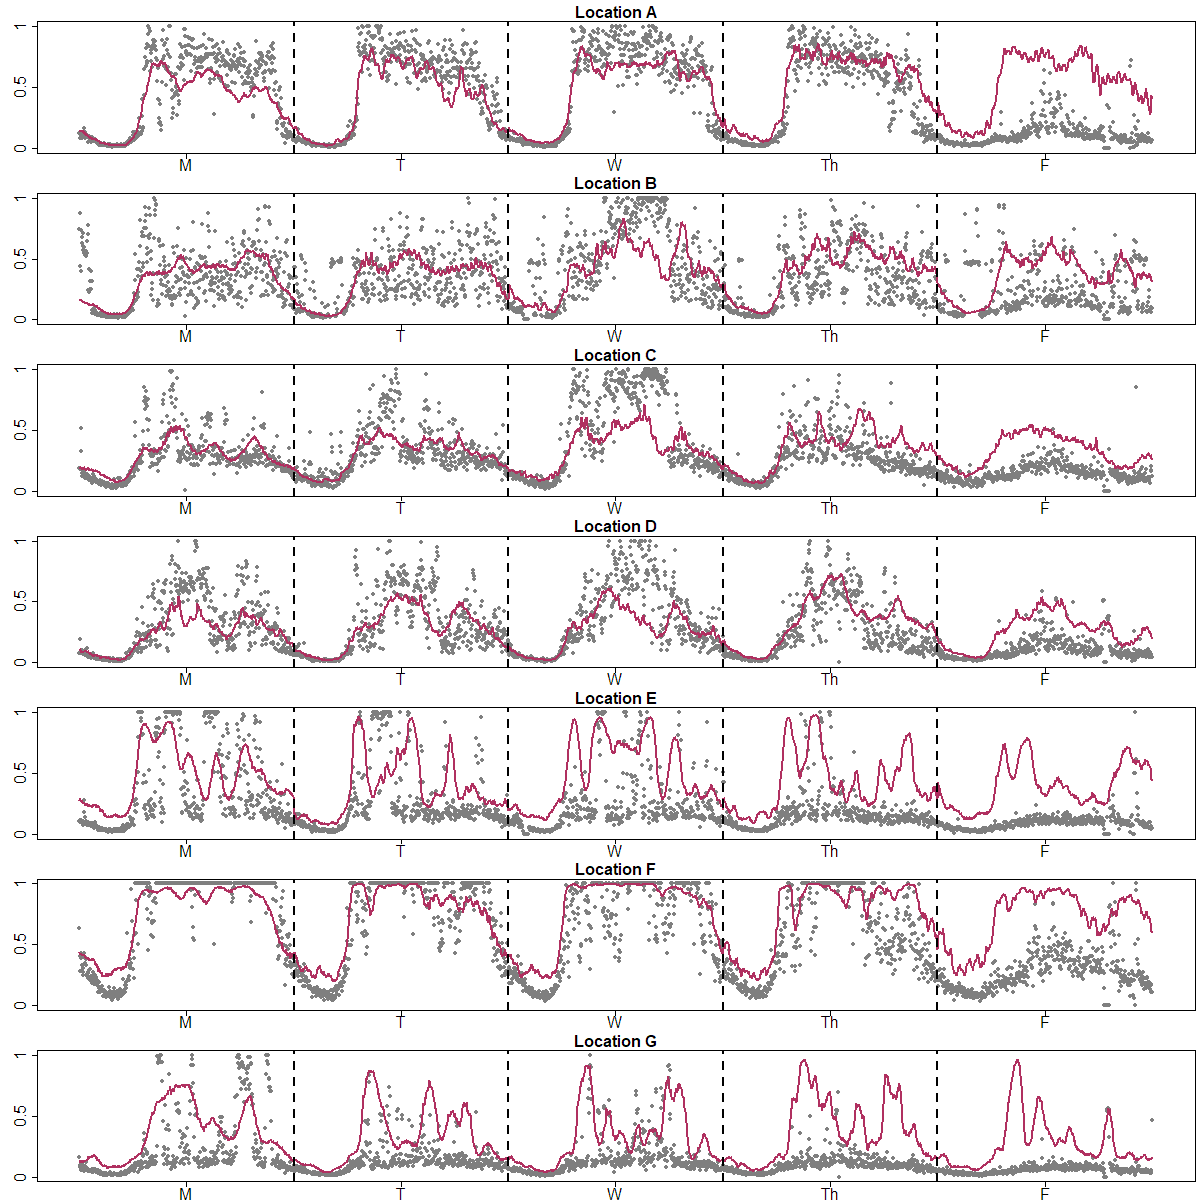
\includegraphics[width=\textwidth]{SEASESTPlots}
\label{fig:SEASESTPlots}
\end{figure}

\begin{figure}[htbp]
\caption{1-Step Ahead Density Forecasts for TAR Models}
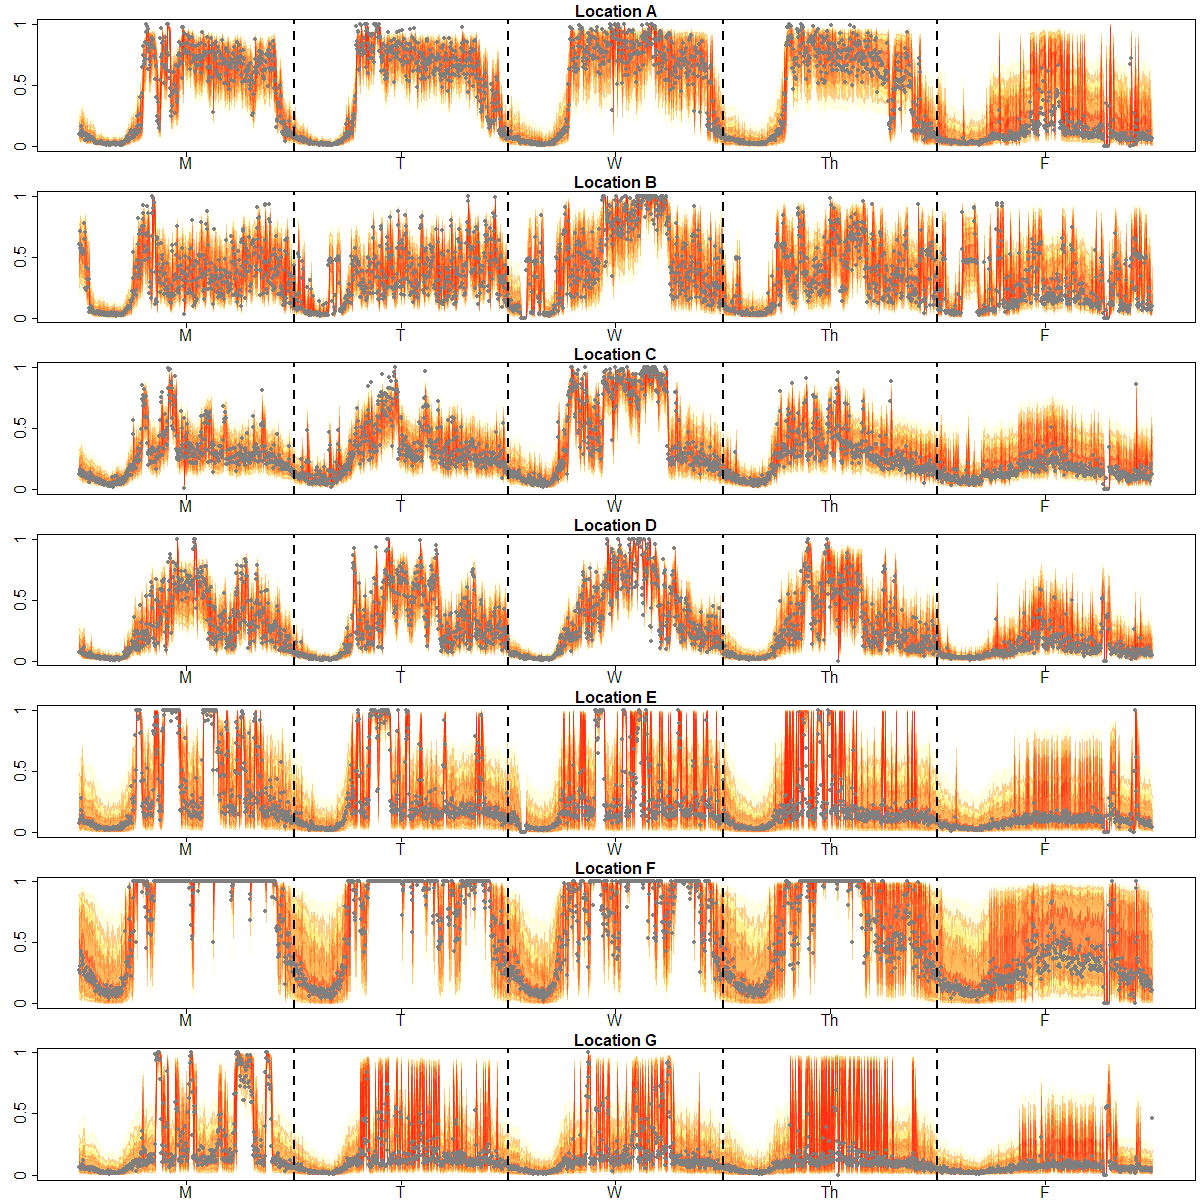
\includegraphics[width=\textwidth]{DENS1Plots}
\label{fig:DENS1Plots}
\end{figure}


\begin{figure}[htbp]
\caption{3-Step Ahead Density Forecasts for TAR Models}
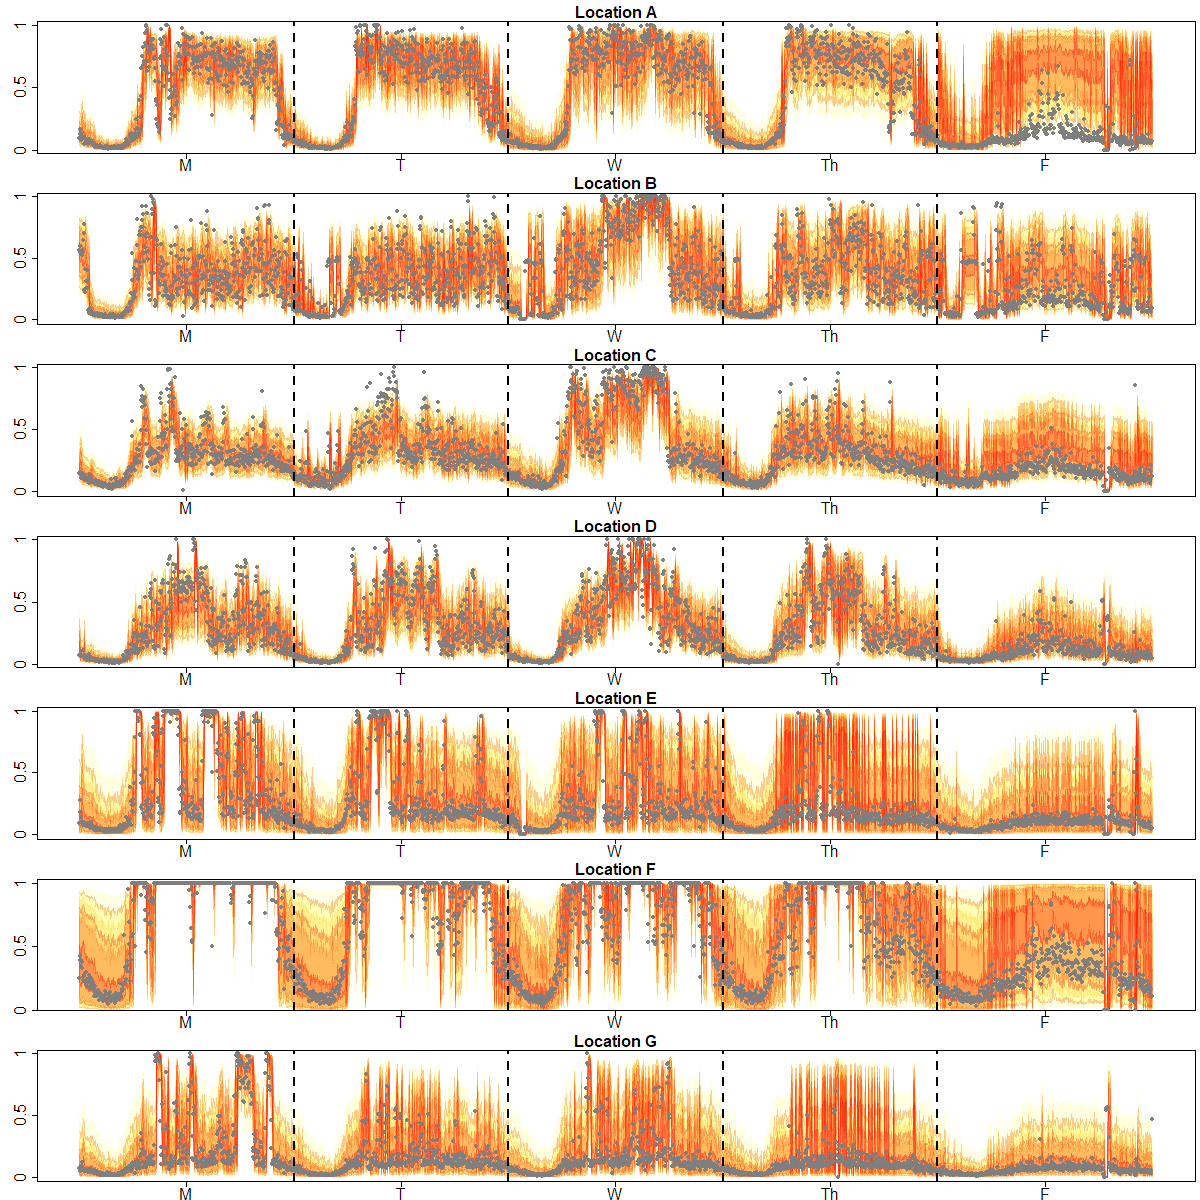
\includegraphics[width=\textwidth]{DENS3Plots}
\label{fig:DENS3Plots}
\end{figure}

\begin{figure}[htbp]
\caption{5-Step Ahead Density Forecasts for TAR Models}
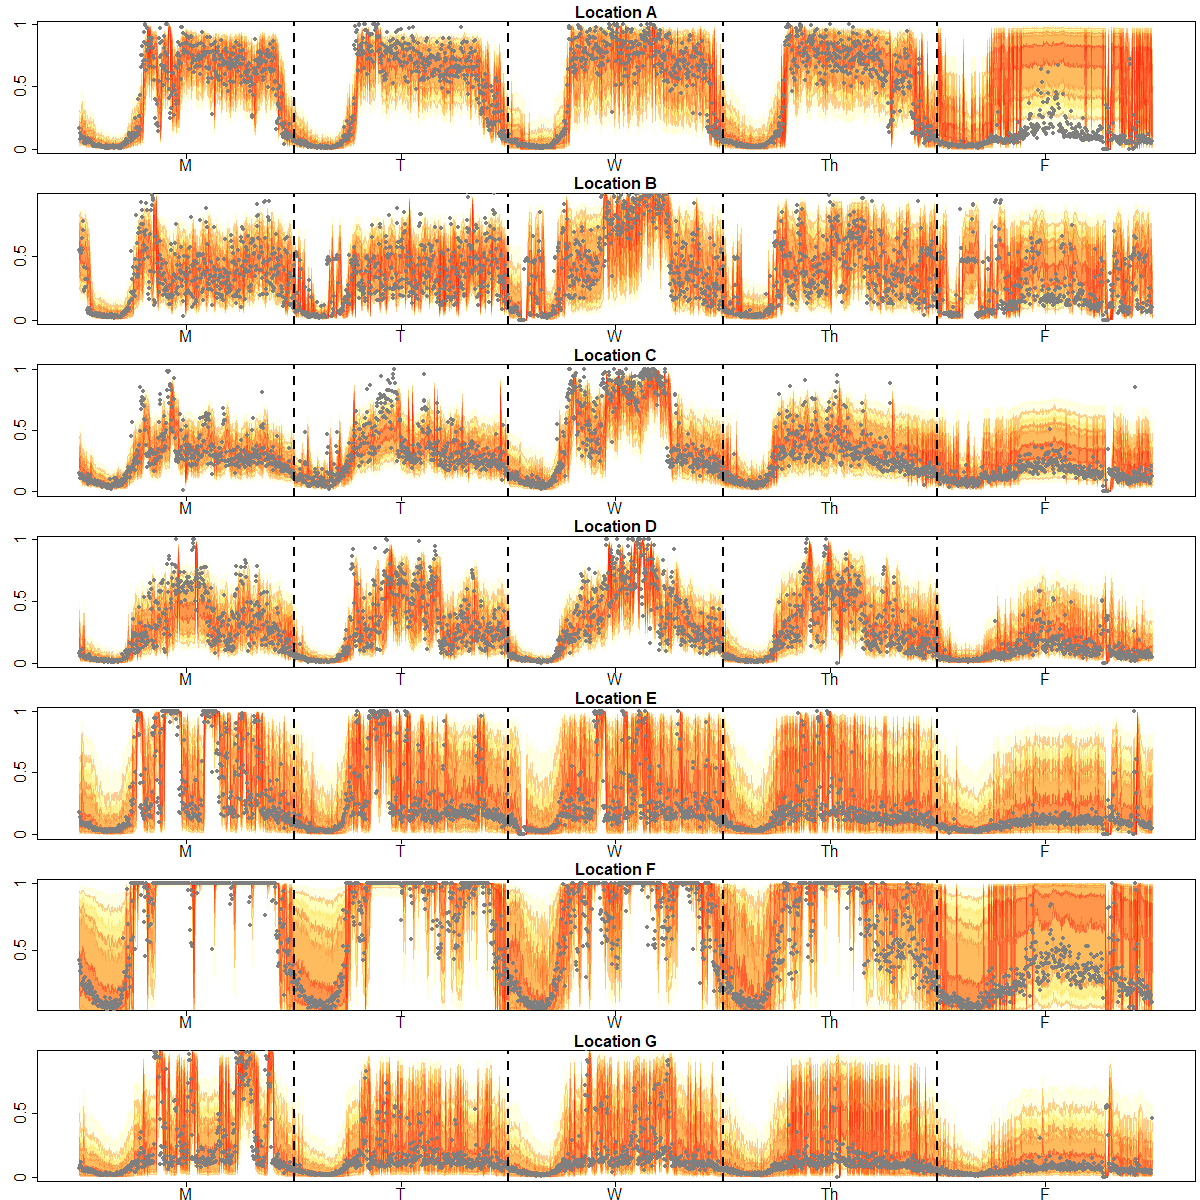
\includegraphics[width=\textwidth]{DENS5Plots}
\label{fig:DENS5Plots}
\end{figure}


Forecasts from both models over this period are evaluated using the mean absolute scaled forecast error (MASFE) metric from \cite{Hyndman2006}. The formulation of MASFE is found in Equation \ref{eq:trafficmase} where $\textrm{MAE}_{RW}(h)$ represents the mean absolute error from a $h$-specific naive random walk (RW) model over the fitting period where $\widehat{O}_{L,t}$ is the observed $O_{L,t-h}$. By scaling errors using $\textrm{MAE}_{RW}(h)$, TAR can be compared to SEAS and both can be compared to simple naive approaches. Whenever MASFE$(h)<1$, the model produces absolute forecast errors that are, on average, less than the forecast errors from a simple random walk model with no parameters.
\begin{equation}
\label{eq:trafficmase}
  \textrm{MASFE}(h)=\frac{1}{T_h}\sum\limits_{t=P+h}^{480}\left|\frac{O_{L,t}-\widehat{O}_{L,t}}{\textrm{MAE}_{RW}(h)}\right|
\end{equation}

Tables \ref{tab:trafficmase1}, \ref{tab:trafficmase3}, and \ref{tab:trafficmase5} compares final TAR and SEAS models for all days and locations at horizons $h\in \{1,3,5\}$, respectively. Multiple-regime TAR models consistently outperform SEAS profiles at all locations and days when forecasting 1-step ahead. For 3-step ahead forecasts, the SEAS model for Tuesday at location $C$ has a smaller MASFE, by a negligible amount. For 5-step ahead forecasts, more occurrences of SEAS producing forecasts, as good or better, than TAR are observed. The opposite pattern is exhibited for $h$-specific RW models. For 1-step ahead forecasts, MASFE$>1$ for many of the models. As the horizon $h$  increases, a clear advantage of using more complicated models (TAR and SEAS) to capture nonlinear and/or seasonal dynamics is notices. This is generally true except for locations $E$, $F$, and $G$ where traffic occupancies are considerably more difficult to model which is visually indicated by the wide credible regions in Figures \ref{fig:DENS1Plots}, \ref{fig:DENS3Plots}, and \ref{fig:DENS5Plots}.



\begin{table}[htbp]
\scriptsize
\centering
\caption{1-Step Ahead MASFE Forecast Comparison}
\begin{tabular}{c|rccccccc}
  \hline
  & & \multicolumn{7}{c}{Location}\\
  \cline{5-7}
Day & Model & A & B & C & D & E & F & G \\ 
  \hline
  \multirow{2}{*}{M} & TAR & 1.02 & 1.10 & 0.88 & 1.07 & 1.87 & 0.81 & 1.48 \\ 
  & SEAS & 1.80 & 1.47 & 1.15 & 1.43 & 4.02 & 1.57 & 3.66 \\ 
  \hline
  \multirow{2}{*}{T}  & TAR & 0.90 & 1.05 & 1.04 & 0.98 & 1.36 & 1.03 & 1.95 \\ 
  & SEAS & 1.35 & 1.36 & 1.22 & 1.46 & 3.36 & 1.65 & 3.29 \\ 
  \hline
   \multirow{2}{*}{W} & TAR & 1.04 & 1.11 & 0.91 & 0.97 & 2.27 & 1.86 & 1.55 \\ 
   & SEAS & 1.39 & 2.01 & 2.18 & 1.61 & 4.65 & 2.90 & 2.80 \\ 
  \hline
 \multirow{2}{*}{Th} & TAR & 0.93 & 0.89 & 0.82 & 0.92 & 1.48 & 1.52 & 1.83 \\ 
   & SEAS & 1.44 & 1.43 & 1.51 & 1.42 & 3.98 & 2.74 & 4.07 \\ 
  \hline
  \multirow{2}{*}{F} & TAR & 1.80 & 1.08 & 1.01 & 0.85 & 1.45 & 2.40 & 1.16 \\ 
   & SEAS & 4.77 & 2.23 & 1.98 & 1.83 & 4.37 & 6.24 & 3.78 \\ 
   \hline
\end{tabular}
\label{tab:trafficmase1}
\end{table}




\begin{table}[htbp]
\scriptsize
\centering
\caption{3-Step Ahead MASFE Forecast Comparison}
\begin{tabular}{c|rccccccc}
  \hline
    & & \multicolumn{7}{c}{Location}\\
  \cline{5-7}
Day & Model & A & B & C & D & E & F & G \\ 
  \hline
  \multirow{2}{*}{M} & TAR & 0.94 & 1.06 & 0.88 & 1.13 & 1.85 & 0.88 & 1.50 \\ 
   & SEAS & 1.36 & 1.17 & 0.93 & 1.14 & 2.91 & 1.19 & 2.57 \\ 
   \hline
  \multirow{2}{*}{T} & TAR & 0.87 & 1.04 & 0.96 & 1.03 & 1.46 & 1.15 & 1.21 \\ 
   & SEAS & 1.04 & 1.06 & 0.91 & 1.10 & 2.24 & 1.22 & 2.15 \\ 
   \hline 
  \multirow{2}{*}{W} & TAR & 1.09 & 1.15 & 1.10 & 0.99 & 1.75 & 2.00 & 1.26 \\ 
   & SEAS & 1.15 & 1.61 & 1.69 & 1.21 & 2.94 & 2.24 & 1.71 \\ 
   \hline
 \multirow{2}{*}{Th}  & TAR & 0.90 & 0.96 & 0.82 & 0.93 & 1.88 & 1.47 & 1.14 \\ 
   & SEAS & 1.15 & 1.09 & 1.14 & 1.03 & 2.69 & 1.96 & 2.68 \\ 
  \hline
  \multirow{2}{*}{F} & TAR & 3.04 & 1.09 & 1.00 & 0.66 & 1.14 & 2.47 & 0.92 \\ 
   & SEAS & 3.53 & 1.57 & 1.42 & 1.33 & 3.12 & 4.35 & 2.42 \\ 
   \hline
\end{tabular}
\label{tab:trafficmase3}
\end{table}




\begin{table}[htbp]
\scriptsize
\centering
\caption{5-Step Ahead MASFE Forecast Comparison}
\begin{tabular}{c|rccccccc}
  \hline
    & & \multicolumn{7}{c}{Location}\\
  \cline{5-7}
Day & Model & A & B & C & D & E & F & G \\ 
  \hline
  \multirow{2}{*}{M} & TAR & 0.94 & 0.99 & 0.89 & 1.12 & 1.97 & 0.86 & 1.68 \\ 
   & SEAS & 1.24 & 1.06 & 0.88 & 1.06 & 2.46 & 1.08 & 2.17 \\ 
  \hline
  \multirow{2}{*}{T}  & TAR & 0.81 & 1.05 & 0.95 & 1.00 & 1.47 & 1.13 & 1.15 \\ 
   & SEAS & 0.95 & 0.95 & 0.85 & 0.99 & 1.85 & 1.07 & 1.77 \\ 
  \hline
  \multirow{2}{*}{W}  & TAR & 1.02 & 1.12 & 1.04 & 0.99 & 1.67 & 1.94 & 1.26 \\ 
   & SEAS & 1.01 & 1.44 & 1.56 & 1.12 & 2.30 & 1.95 & 1.44 \\ 
  \hline
  \multirow{2}{*}{Th}  & TAR & 0.84 & 0.98 & 0.82 & 0.87 & 1.51 & 1.48 & 1.22 \\ 
   & SEAS & 1.05 & 1.03 & 1.07 & 0.94 & 2.13 & 1.73 & 2.24 \\ 
  \hline
  \multirow{2}{*}{F}  & TAR & 2.85 & 1.20 & 0.88 & 0.70 & 1.26 & 2.52 & 1.00 \\ 
   & SEAS & 3.07 & 1.48 & 1.33 & 1.19 & 2.59 & 3.82 & 2.01 \\ 
   \hline
\end{tabular}
\label{tab:trafficmase5}
\end{table}




\section{Conclusion}
Short-term forecasting of traffic occupancy is useful in real-time monitoring of a network. The nonlinearities present in the data make it difficult to get precise predictions. Daily traffic occupancy cycles between periods of free flow to periods of congestion. Threshold autoregressions capture many of these nonlinearities by using separate autoregressive processes to model dynamics for different states. Since occupancy is quality measure of traffic flow, this endogenous characteristic can characterize the regimes. 

The general estimation difficulties of TAR models lead users to fix the number of regimes prior to fitting the model. In this application to traffic occupancy, the number of thresholds $m$ is fixed and a high dimensional linear model matrix that nests many TAR models with regimes less than $m+1$ is constructed. Sparse estimation of the coefficients not only identifies the optimal number of regimes, but also selects the thresholds. After fixing the maximum autoregressive order $P$ and choosing the $m$ thresholds, we present a three step model building procedure that automates subset TAR$(P)$ selection. 

Using a metric scaled by the MAE of a naive random walk evaluated from the training period, advantages of TAR models over sparse periodic seasonal signals are discovered for forecasting 3, 9, and 15 minutes ahead. Nevertheless, there is room for improvement. The outlined posterior prediction projective method for subset selection of TAR requires the assumption that errors follow a \textit{normal} distribution with zero mean and constant variance. Although we estimate linear models using logit transformed data and capture some of the heteroskedasticity when we convert back to the original scale, it may be advantageous to modify the approaches with robust \textit{Student t} errors, within-regime homoskedasticity, or stochastic volatility models for the variance. 
























\chapter{REGULARIZATION METHODS FOR SUBSET ARMA SELECTION}

\section{INTRODUCTION}

Let $\{y_t: t=1,2,\cdots,T\}$ be a sequentially observed discrete and equally-spaced sample from a weakly stationary and homoskedastic process $\{Y_t:t=\cdots,-1,0,1,\cdots\}$. For the purpose of forecasting future realizations i.e. $\hat{y}_{t+h}$ where $h\in\mathbb{N}$, we estimate a model for $\{Y_t\}$ of the general form $Y_{t}=f(Y_{t-1},Y_{t-2},\cdots,Y_{t-p},\epsilon_{t-1},\epsilon_{t-2},\cdots,\epsilon_{t-q})+\epsilon_t$ from known $\{y_t\}$. Under homoskedasticitcy, $\{\epsilon_t\}$ is assumed to be white noise with mean 0 and variance $\sigma^2$.  Finite order parameters $p$ and $q$  quantify the extent of past information of $\{Y_t\}$ and $\{\epsilon_t\}$, respectively, helpful for prediction. Define $m=\max\{p,q\}$. In most cases, $m$ is small relative to $T$; however, when cyclical phenomenon is detected, $m=S$ where $S$ is the seasonal periodicity. The latter scenario often produces long gaps between relevant past information for model fit.

Common practice subset of the seasonal autoregressive moving average (SARMA) process is most commonly used for modeling the temporal dynamics of $\{y_t\}$ to forecast future unknown realizations. 

expressed in Equation \ref{eq:sarma} and abbreviated SARMA$(p,q)\times(P,Q)_{S}$ .


\begin{equation}
\label{eq:sarma}
\Phi(B^S)\phi(B)y_t=\Theta(B^S)\theta(B)\epsilon_t
\end{equation}

\begin{equation}
\label{eq:arma}
\bigg(1-\sum\limits_{i=1}^{p}\phi_{i}B^i\bigg)y_{t}=\bigg(1+\sum\limits_{j=1}^{q}\theta_{j}B^j\bigg)\epsilon_{t}
\end{equation}

In this parameterization, we utilize the backshift operator $B$ where $B^ky_{t}=y_{t-k}$. Furthermore, we assume $y_t$ has been centered and $\{\epsilon_t\}$ is white noise with zero mean and constant variance $\sigma^2$. Real-world application of the ARMA($p$,$q$) model to temporally dependent data relies on some form of model selection since model misspecification  

 Classically, the focus of model selection in this context identification of the AR order $p$ and MA order $q$.

For the purpose of subset ARMA selection, we express the model in Equation \ref{eq:arma} as the linear matrix form in Equation \ref{eq:linarma}. Under this $\bm{y}=\bm{X}\bm{\beta}+\bm{\epsilon}$
\begin{equation}
	\label{eq:linarma}
	\begin{bmatrix} y_m\\y_{m+1}\\y_{m+2}\\ \vdots\\ y_T\\ \end{bmatrix} =
	\begin{bmatrix} y_{m-1} & \cdots & y_{m-p} &
					\epsilon_{m-1} & \cdots & \epsilon_{m-q} \\
					y_{m-2} & \cdots & y_{m-p-1} &
					\epsilon_{m-2} & \cdots & \epsilon_{m-q-1} \\
					\vdots & \ddots & \vdots &
					\vdots & \ddots & \vdots & \\
					y_{T-1} & \cdots & y_{T-p} &
					\epsilon_{T-1} & \cdots & \epsilon_{T-q} \\
	\end{bmatrix}
	\begin{bmatrix} \phi_1\\ \phi_2\\ \vdots\\ \phi_p\\ \theta_1 \\
  						\theta_2\\ \vdots	\\ \theta_q\\ \end{bmatrix} +
  	\begin{bmatrix} \epsilon_m\\ \epsilon_{m+1}\\ \epsilon_{m+2}\\ \vdots\\ \epsilon_T\\ \end{bmatrix}
\end{equation}




\cite{Chen2011} 


\section{METHODS}

\subsection{ADAPTIVE LASSO}
The lease absolute shrinkage and selection operator (LASSO) of \cite{Tibshirani1996}.The $\L_1$ penalty is limited when highly correlated predictor variables are considered in model matrix $\bm{X}$.

Generally, the LASSO estimator $\hat{\bm{\beta}}$ is conditionally consistent for $\bm{\beta}$ 
\cite{Zhao2006}.
In \cite{Zou2006}

\subsection{ADAPTIVE ELASTIC NET}


\subsection{OPTIONS FOR SELECTING TUNING PARAMETERS}
Let $\mathcal{M}_1$ and $\mathcal{M}_2$ represent two competing subset ARMA($p$,$q$) models

Penalized estimation via E-NET of autoregressive parameters $\hat{\bm{\phi}}_{\lambda,\alpha}$ and $\hat{\bm{\theta}}_{\lambda,\alpha}$ using LASSO or ENET are dependent on selection of tuning parameters $\lambda$ and  $\alpha$.

\subsubsection{SELECTION BASED ON AIC OR BIC}

\subsubsection{SELECTION BASED ON OOS FORECAST EVALUATION}

\subsubsection{SELECTION BASED ON CV FOR INDEPENDENT DATA}

\subsubsection{SELECTION BASED ON CV FOR DEPENDENT DATA}


In the time series context, the best model minimizes forecasting error for future observations  unrealized during the model building  

\subsection{BAYESIAN PREDICTIVE POSTERIOR PROJECTION METHOD}
The classic method for model selection within the Bayesian framework begins with a reparameterization of the AR and MA coefficients to $\phi_i^*=\phi_i$ and $\theta_j^*=\theta_j$.

Since the introduction of Bayesian LASSO, research in Bayesian regularization methods has exploded over the last ten years. Bayesian methods analogous to adaptive lasso \citep{Leng2014}, elastic net \citep{Li2010a}, and adaptive elastic net \citep{Stankiewicz2015} have been introduced and applied. \cite{Polson2010}





\section{MONTE CARLO SIMULATIONS}
Multiple Monte Carlo studies are performed to evaluate the effectiveness of the three methods on subset ARMA selection. Consider the three time series $\{y_{1,t}\}$, $\{y_{2,t}\}$, and $\{y_{3,t}\}$ generated by the Gaussian ARMA processes expressed in Equations \ref{eq:simarma1}, \ref{eq:simarma2}, and \ref{eq:simarma3}.
\begin{equation}
	\label{eq:simarma1}
	y_{1,t}=0.8y_{1,t-1}+0.7y_{1,t-6}-0.56y_{1,t-7}+\epsilon_{1,t}
\end{equation}
\begin{equation}
	\begin{split}
	\label{eq:simarma2}
	y_{2,t}&=0.8y_{2,t-1}+0.7y_{2,t-6}-0.56y_{2,t-7}\\
	&+0.8\epsilon_{2,t-1}+0.7\epsilon_{2,t-6}+0.56\epsilon_{2,t-7}+\epsilon_{2,t}
	\end{split}
\end{equation}
\begin{equation}
	\label{eq:simarma3}
	y_{3,t}=0.8\epsilon_{3,t-1}+0.7\epsilon_{3,t-6}+0.56\epsilon_{3,t-7}+\epsilon_{3,t}
\end{equation}
The errors $\{\epsilon_{1,t}\}$, $\{\epsilon_{2,t}\}$, and $\{\epsilon_{3,t}\}$ are i.i.d. Gaussian processes with $0$ mean. These three ARMA models are equivalent to the multiplicative seasonal models of period 6 estimated in \cite{Chen2011} using adaptive Lasso. 





\section{APPLICATION}






\section{CONCLUSION}





%-----------------------back matter

{\singlespace
% Making the references a "part" rather than a chapter gets it indented at
% level -1 according to the chart: top of page 4 of the document at
% ftp://tug.ctan.org/pub/tex-archive/macros/latex/contrib/tocloft/tocloft.pdf
\addcontentsline{toc}{part}{REFERENCES}
\bibliographystyle{asudis}
\bibliography{phd}}

\renewcommand{\chaptername}{APPENDIX}
\addtocontents{toc}{APPENDIX \par}
\appendix
\chapter{R Code for Chapter 2}
\label{appendix1}
\lstinputlisting[language=Renhanced,basicstyle=\scriptsize]{IJF_Paper_Code.R}



\end{document}
